% Main manuscript file

\documentclass{is295}
\usepackage[bookmarks=true,linktoc=all,hidelinks]{hyperref} %for hyperlinks
\usepackage[utf8]{inputenc}
\usepackage{longtable}

\usepackage{array}
\usepackage{xcolor}
\usepackage{float}
\usepackage{pdfpages}
\usepackage{etoolbox}

% Tables (wrapping + nice rules)
\usepackage{tabularx,booktabs,threeparttable,makecell,ragged2e}
\newcolumntype{Y}{>{\RaggedRight\arraybackslash}X}
\setlength{\tabcolsep}{3.5pt}
\renewcommand{\arraystretch}{1.12}

% Caption settings are applied globally in is295.cls.

% Apply consistent table formatting throughout the manuscript
\AtBeginEnvironment{table}{\footnotesize}
\AtBeginEnvironment{longtable}{\footnotesize}
\AtBeginEnvironment{tabular}{\footnotesize}
\AtBeginEnvironment{tabularx}{\footnotesize}

% Define a smaller font for the table
\newcommand{\smalltable}{\fontsize{9pt}{11pt}\selectfont}

%\usepackage{showframe} %for debugging the margins
                              
%Replace the values here, various commands depend on this variables  
\renewcommand{\TITLE}{SPONSOR MANAGEMENT AND LETTER OF GUARANTEE (LoG) COVERAGE INTEGRATION SYSTEM FOR INTERNATIONAL SCHOOL MANILA (ISM)}
\renewcommand{\AUTHOR}{RENALD E. CRUZ}
\renewcommand{\DEGREE}{MASTER OF INFORMATION SYSTEMS}
\renewcommand{\ADVISER}{KATRINA JOY M. ABRIOL-SANTOS}
\renewcommand{\FACULTY}{Faculty of Information and Communication Studies}
\renewcommand{\MONTH}{MAY}
\renewcommand{\YEAR}{2026}
\renewcommand{\DAY}{08}

% Choose between YES and NO here
\renewcommand{\INVENTION}{YES/NO}
\renewcommand{\PUBLICATION}{YES/NO}
\renewcommand{\CONFIDENTIAL}{YES/NO}
\renewcommand{\FREE}{YES/NO}
% ---------------------

\newcommand{\PROGRAMCHAIR}{DR. RIA MAE H. BORROMEO}
\newcommand{\DEAN}{DR. ROBERTO B. FIGUEROA, JR.}

\begin{document}
	\emergencystretch 3em
	\clubpenalty=10000
	\widowpenalty=10000
	\displaywidowpenalty=10000
	\begin{frontmatter}
            
		%TITLE PAGE
		\maketitle

            %PERMISSION PAGE
            \include{permission}

            %APPROVAL PAGE
            \include{approval}
            
		%ACKOWLEDGEMENT
            % Put your acknowledgement here

\begin{acknowledgement}

The researcher would like to express his gratitude to the Professional Development assistance that was provided by the \textbf{International School Manila}, which allowed the researcher to be able to undertake this course and conduct this capstone project. The support of the institution reflects its recognition of the importance of continuing learning, professional development and strengthening of systems to support school operations. 

Special thanks to the people inside \textbf{International School Manila}, particularly those in \textbf{Finance} and \textbf{Accounting}, \textbf{Admissions}, \textbf{IT} and \textbf{Student Charging operations}, who provided their process knowledge, participated in consultations and pilot testing of the system. Their practical experience proved to be very valuable in the formulation of the project requirements and keeping the study relevant with the institutional needs. 

The researcher would also like to express heartfelt gratitude to \textbf{Finance Director Joel Songco} for his assistance, encouragement and guidance in the development and pilot validation of this project. His support enabled the project to be placed in the needs of Finance and the overall billing process of the institution. 

The researcher also wishes to thank the adviser, \textbf{Katrina Joy M. Abriol-Santos}, for her insight, patience and constant feedback that guided the direction and rigor of this research. The authors also gratefully acknowledge the support and comments of the IT Developers, the reviewers, administrative staffs, and IS 295 classmates that assisted by providing comments, suggestions, and peer reviews that helped improve the pilot web application deployed and the manuscript. 

Special thanks to \textbf{Paolo Escotido} and \textbf{Jefferson Legaspi}, co-worker and classmates, respectively, of the researcher for the technical and personal assistance given during this course and during the completion of this capstone project. 

Lastly, heartfelt thanks go to the researcher’s \textbf{family} and \textbf{friends} for their patience, understanding, help, and encouragement while this deployed pilot web application and manuscript was completed.
\end{acknowledgement}
		
            %ABSTRACT
            % Put your abstract here

\begin{abstractwithpageno}
International School Manila has four separate systems for handling sponsorship billing and Letter of Guarantee (LoG) coverage: PowerSchool (SIS), the Student Charging Portal (SCP), NetSuite (ERP), and the Online Billing System (OBS). Prior to the development of this project, coverage decisions were manually interpreted at charge entry and this could lead to inconsistent assignments to \textbf{Bill-To}, causes for delay in the correction process, lack of audit trails and further reconciliation efforts. The project created and implemented a pilot \textbf{Sponsor Management and LoG Coverage Integration System} that combines all the master data of sponsors, tracks LoG records, handles workflows based on the roles and assesses coverage using the \textbf{deterministic business rules}.

The \textbf{deployed pilot web application} was done with ASP.NET Core including REST API endpoints, role-based authentication for Administrator, Admissions and Cashier users, local credentials for authentication for ISM staff accounts, and Azure deployment for production-style validation. The system enables the management of sponsor profiles, prevention of sponsor duplication, creation and activation of LoG, sponsor change requests, sponsor views, coverage preview, creation of audit trail and reporting support. The web interface has been responsive and is \textit{PWA-ready}, but has not been fully developed as a Progressive Web App as the \textit{PWA installable features}, \textit{service worker caching}, \textit{offline behavior} and the \textit{web app manifest} were not in the scope of the pilot.

A total of \textbf{110 test cases} were found in total, of which \textbf{95 passed}, \textbf{12 noted} and \textbf{3 known non-critical items} were noted; none of them were critical or blocking. \textbf{60 user acceptance testing (UAT) workflow scenarios} were verified; \textbf{54 were successful} and \textbf{6 were non-blocking issues} for refinement. The proven workflows covered sponsor search, sponsor maintenance, creation and viewing of the LoG, coverage check, restricted access, report generation, and sponsor self-service actions. There are minor usability and validation issues such as the delayed LoG reassignment display after sponsor merge, the lack of visibility for attachments in one change-request flow, unclear confirmation messages, incomplete report header metadata, and improved sponsor access-error messages.

The pilot proved to show that existing manual interpretation can be minimised, governance is enhanced, audit preparedness is improved and a practical roadmap towards production integration with current ISM systems is achieved with a centralized \textbf{Sponsor Master} and \textbf{deterministic coverage engine}. The pilot web application deployed is a working example that shows that there is no need to replace ISM's existing core platforms, and that consistent and explainable decisions on coverage of sponsors can be made. This pilot web application is a working example that demonstrates that consistent and explainable decisions on coverage of sponsors can be made without replacement of existing ISM core platforms.
\end{abstractwithpageno}
		
		%TABLE OF CONTENTS
		\maketableofcontents
		
		%LIST OF TABLES
		\makelistoftables

		%LIST OF FIGURES
		\makelistoffigures

	\end{frontmatter}
	
	%BODY OF MANUSCRIPT HERE (Use up to 3 levels only, (sec -> subsec -> subsubsec)
	\begin{mainmatter}
		
            %INTRODUCTION
            % introduction.tex

\section{INTRODUCTION}

\subsection{BACKGROUND OF THE PROJECT}

    To address these issues in sponsorship billing, which persists in the field, and the need to have reliable financial records, this study proposes an integration-first \textbf{SPONSOR MANAGEMENT AND LETTER OF GUARANTEE (LoG) COVERAGE INTEGRATION SYSTEM FOR INTERNATIONAL SCHOOL MANILA (ISM)}. The system does not look at sponsorship coverage as a local system, it also looks at it as a common institutional reference. It utilizes a centralized \textbf{Sponsor Master} and a uniform rules engine to cover the rules and parameters for student charges, as well as uniform identifiers that are synchronized across \textbf{PowerSchool} as the Student Information System (SIS) that holds the primary student profile, \textbf{NetSuite} as the finance system, which records charges and maintains the student ledger, the in-house \textbf{Student Charging Portal}, which processes charges by students, and the \textbf{Online Billing System}, which displays statements of account to parents and sponsors.
    
    International School Manila has four systems in place to bill students and these were implemented at various times due to various operational needs. \textbf{PowerSchool} contains enrollment and demographic information. The \textbf{Student Charging Portal} is used by front-line staff to make itemized charges. These charges are recorded in \textbf{NetSuite} and included in the student ledger for financial reporting. The ledger entries then become statements to parents and sponsors via the \textbf{Online Billing System}. Sponsorship billing is available in this multi-system environment and is backed by \textbf{Letters of Guarantee (LoG)} issued by sponsors to specify items and/or categories that they will sponsor.
    
    Each time a charge entry is added to the \textbf{Student Charging Portal}, operators review each LoG and decide if a line item is covered, and then indicate if it is a \textbf{Bill-To} by the sponsor or parent. These decisions go through the integration chain (charges are added into \textbf{NetSuite} and the \textbf{Online Billing System} shows the resulting statement of account for parents/sponsors). Staff use spreadsheet and 2 comma-separated value (CSV) files to manually match records between platforms and ensure the these platforms are synchronized.
 
    \begin{figure}[H]
        \centering
        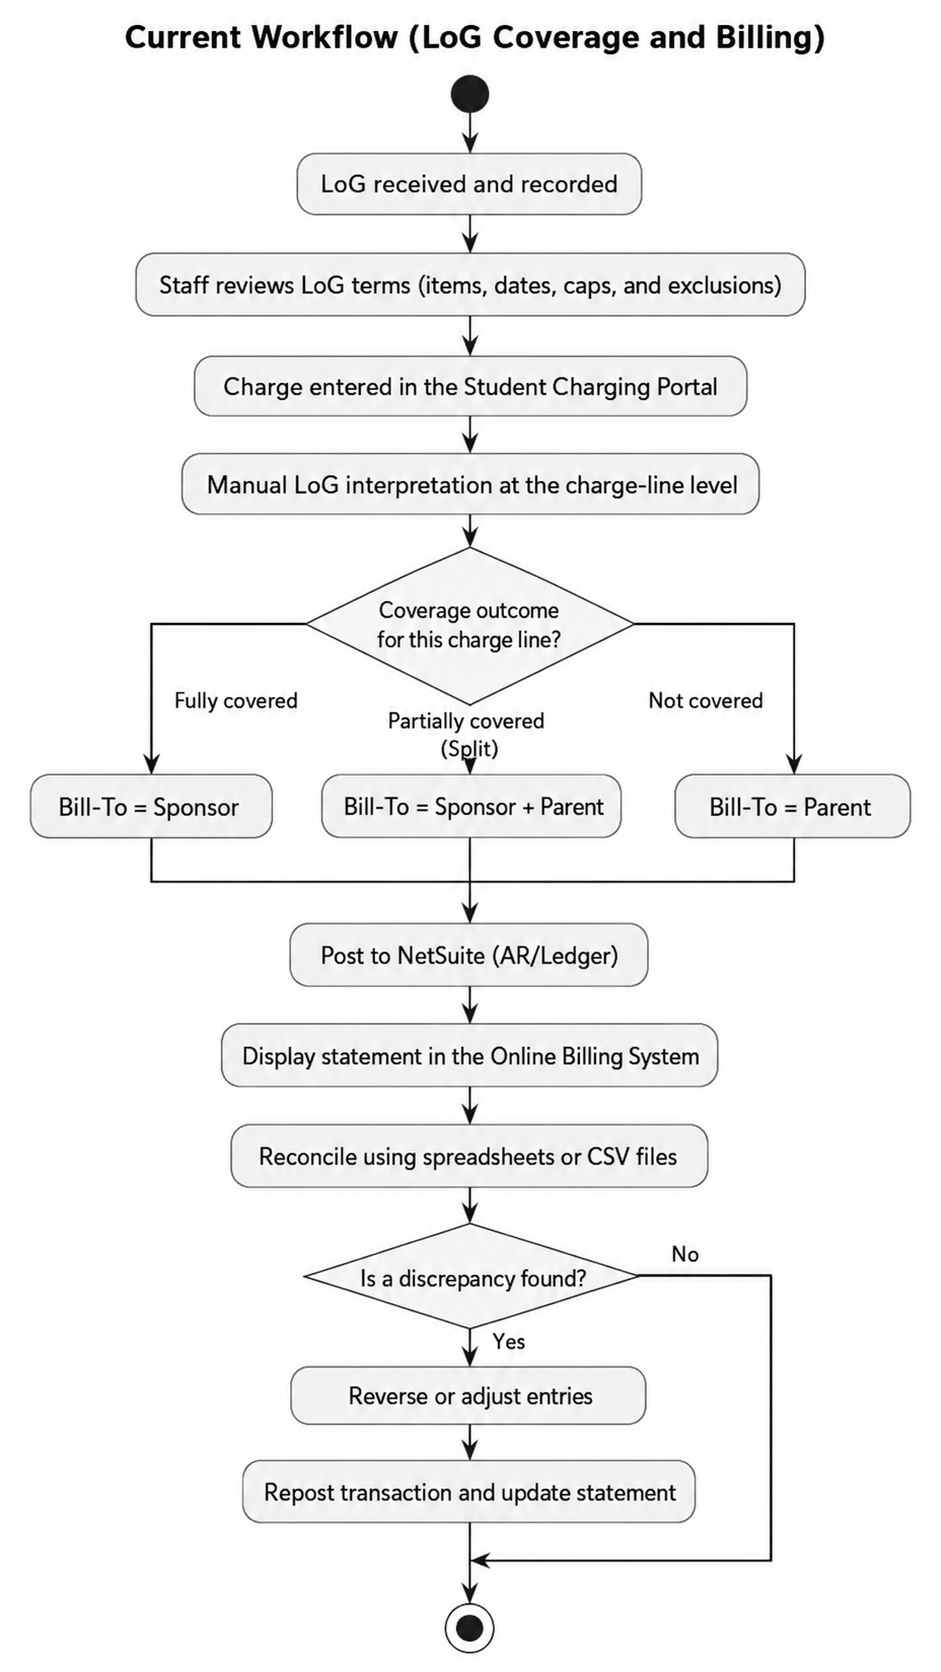
\includegraphics[width=0.95\linewidth,height=0.82\textheight,keepaspectratio]{images/Current Workflow.png}
        \caption{Current manual LoG coverage and billing workflow}
        \label{fig:current-workflow}
    \end{figure}

    \noindent Figure~\ref{fig:current-workflow} shows the current manual LoG coverage and billing workflow. The decision point clarifies the three possible outcomes for each charge line: full sponsor coverage, partial sponsor-parent coverage, and no sponsor coverage. These outcomes determine whether the Bill-To value is assigned to the sponsor, split between sponsor and parent, or assigned to the parent.

    With the passage of time, this manual interpretation and “file” based reconciliation has proven to be very problematic. This can make it hard to keep connections between spreadsheet references and unofficial notes with authoritative information. There is some variation among staff in how they interpret similar LoG provisions, and may result in a variety of \textbf{Bill-To} decisions on similar charges. Late postings, inaccurate postings, and missing documents decrease the trust in the student ledger, make reconciling more difficult and puts the institution at risk of audit and regulatory exposure. The concerns are set against a backdrop of a regulatory framework which demands accuracy, transparency and accountability.  

    Student information data needs to be synced from ISM to a third party SIS, billing capture to an in-house portal, statements to an in-house billing system and accounting data to a third-party finance system. It should also meet the requirement of the BIR policy on \textbf{‘Ease of Paying Taxes' (EoPT)} which requires the billing to be kept in a well documented and clear manner. A lack of person-centredness and disconnection around the amount of coverage of sponsorships within this context leads to tension in operations and governance. There are other solutions, but they have their own major cost/benefit considerations for ISM. 
    
    One way is to have a single vendor system which integrates student records, billing, ledgers and accounting in a single enterprise resource planning (ERP) application. This would drastically reduce the number of applications, but would require a massive migration, re-negotiation of current integrations and customization of ISM processes to meet the recommended processes of the vendor, which may differ from ISM's integration of \textbf{PowerSchool)}, \textbf{NetSuite)} and in-house processes. 
    
    The second option would be to use a dedicated sponsorship administration software or billing portals for sponsorships which are specifically created for billing and collections. These tools can aid in payment tracking but can continue to require manual interpretation of the charge when payments are inputted to the system and manual 4 reconciliation in a spreadsheet, thus perpetuating the lack of consistency charge-to-Bill. 
    
    The third approach is to continue improving the spreadsheet-based process with more stringent templates and more oversight of the review process. This approach remains ‘manual', labour intensive, scaleable and scalable to audit, however. These are not to be confused with the deployed \textbf{SPONSOR MANAGEMENT AND LETTER OF GUARANTEE (LoG) COVERAGE INTEGRATION SYSTEM FOR INTERNATIONAL SCHOOL MANILA (ISM))} which is not meant to take the place of the school's main systems. 
    
    It instead aims to address the issue of inconsistencies – lack of a single, rule-based sponsorship coverage source. The system does not replace \textbf{PowerSchool)}, \textbf{NetSuite)} or in-house portals, it is a shared institutional service to determine if there is coverage for the charge and if so, how to cover it is evaluated on every charge that is processed. This allows the line level, deterministic \textbf{Bill-To decisions} to be returned when the charges are entered, reflected as accurate transactions within \textbf{NetSuite)}, and displayed as a definite line of charge in the Online Billing System for parents and sponsors to see. By doing so, the deployed pilot system brings together the best of the existing landscape together with centralized logic and explainable decisions, offering a more practical, lower risk and institution-specific solution compared to undertaking a complete system replacement or a continued reliance on manual spreadsheets.
    \pagebreak

\subsection{DEFINITION OF TERMS}

\begin{description}
    \item[\textbf{AR}] Accounts Receivable.

    \item[\textbf{Azure}] Microsoft Azure, the cloud platform where system services and data are hosted.

    \item[\textbf{Bill-To Designation}] The ultimate decision of who the billing party is for a charge line item. This may be the sponsor, the parent, or both parties for downstream financial posting and statement presentation purposes.

    \item[\textbf{BIR EoPT}] Bureau of Internal Revenue Ease of Paying Taxes.

    \item[\textbf{Cashier}] Staff members who use the sponsor dropdown in PowerSchool (SIS) to tag a student's sponsor from the LoG system.

    \item[\textbf{Coverage Decision}] A determination outcome for a charge line item, classified as Covered, Split, or Not Covered, created when the charge item is created and stored with the reason code and rule version.

    \item[\textbf{Coverage Evaluation}] A rule-based process used to determine whether a sponsor covers a charge line item or charge line item category.

    \item[\textbf{Coverage Rule}] A deterministic rule specifying coverage by category or item, including limits, exceptions, and dates of coverage for the sponsor.

    \item[\textbf{CSV}] Comma-Separated Values, a flat-file format usually used to export and import data.

    \item[\textbf{Deterministic Rules Engine}] A rules-based evaluation component that makes consistent coverage decisions using the same inputs, explicit rule priorities, constraints, and computation logic, without using predictive modeling.

    \item[\textbf{ERP}] Enterprise Resource Planning.

    \item[\textbf{Identifier}] A unique value used to match and synchronize records between systems, such as sponsor IDs and student IDs.

    \item[\textbf{International School Manila}] The school where the Sponsor Management and LoG Coverage Integration System was developed and piloted. 
    
    \item[\textbf{IT Administrator Staff}] that installs integration and schedules. In the target state, they sync the records from the sponsors in the LoG system. 
    
    \item[\textbf{Ledger}] The financial history of charges and related transactions in the finance system. Letter of Guarantee (LoG) A letter from the sponsor outlining the amount of charges to be paid, coverage limits, dates, exclusions, supporting documentation etc.

    \item[\textbf{Letter of Guarantee (LoG)}] A document issued by the sponsor that details the extent of charges the sponsor will pay, including coverage limits, dates, exclusions, and supporting documentation.

    \item[\textbf{NetSuite}] The Finance and Accounting system used to record student charges and maintain the student ledger.

    \item[\textbf{NS}] NetSuite, also referred to as the Enterprise Resource Planning (ERP) system.

    \item[\textbf{OBS}] Online Billing System.

    \item[\textbf{Online Billing System}] The billing system that displays statements of account to parents and sponsors online.

    \item[\textbf{PowerSchool}] The Student Information System (SIS) that stores primary student enrollment and profile information.

    \item[\textbf{PS}] PowerSchool, the Student Information System.

    \item[\textbf{Reason Code}] A machine-readable label that explains a coverage or billing decision.

    \item[\textbf{Rules Engine}] The software component that applies coverage rules to charge entries and generates consistent and explainable results.

    \item[\textbf{SCP}] Student Charging Portal.

    \item[\textbf{SCP Operator}] Staff who enter student charges in SCP and use the coverage decision as the basis for deciding whether or not to cover the charge.

    \item[\textbf{Sponsor}] An outside organization, agency, or person who agrees to pay charges, in full or in part, for an assessed student under an approved Letter of Guarantee (LoG). Sponsorship is defined through billing-rule terms and conditions, including covered charge items or categories, coverage limits, effective dates, exclusions, required documentation, and allocation terms for sponsor and parent responsibility.

    \item[\textbf{Sponsor ID}] The unique identifier of a sponsor in this system.

    \item[\textbf{Sponsor-Parent Allocation}] The calculated way a charge amount is divided between sponsor responsibility and parent responsibility, in amounts and percentages, if applicable.

    \item[\textbf{Sponsor Master}] A single source of synchronized and consistent sponsors, attributes, identifiers and governance controls across PowerSchool, the Student Charging Portal, NetSuite and the Online Billing System.

    \item[\textbf{Statement of Account (SOA)}] An itemized billing statement that includes charges and parent-sponsor responsibilities.

    \item[\textbf{Student Charging Portal}] An in-house system used by staff to create and submit itemized student charges.

    \item[\textbf{Student Information System (SIS)}] Software used to store student enrollment, demographic, and profile information.

    \item[\textbf{Transaction}] A recorded financial event in the finance system, such as a charge entry, that is also shown in billing statements.
\end{description}
\pagebreak

\subsection{OBJECTIVES}

\subsubsection{General Objective}

    To create and implement an \textbf{INTEGRATED SPONSOR MANAGEMENT AND LETTER OF GUARANTEE (LoG) COVERAGE INTEGRATION SYSTEM FOR INTERNATIONAL SCHOOL MANILA (ISM)} that will automate the process of covering Student Charging Portal (SCP) Letter of Guarantee (LoG) in the PowerSchool system.

\subsubsection{Specific Objectives}

\begin{enumerate}
    \item To ensure \textbf{PowerSchool}, \textbf{NetSuite}, the \textbf{Student Charging Portal}, and the \textbf{Online Billing System} are all synchronized and validate sponsor coverage using a common identifier and processing business events like create, update and merge.

    \item To have a real-time, explainable coverage determination in the \textbf{Student Charging Portal (SCP)} that relies on a deterministic rules engine that utilizes sponsor coverage rules when charge is posted and reason codes are provided as human-readable values when a \textbf{Bill-To} determination is made.

    \item To develop a \textbf{Sponsor Master} with centralized sponsor records, coverage policies, limits, effective dates, status values and identifiers that will be used to identify students and track financial transactions in \textbf{PowerSchool} and \textbf{NetSuite}.

    \item To record proper \textbf{Bill-To} in \textbf{NetSuite} and the \textbf{Online Billing System}, support BIR audit and compliance requirements, and record proper sponsor/parent allocation in student ledger and general ledger.

    \item To ensure data quality and governance in the \textbf{Sponsor Master}, by validating required fields, attributes for classification and by maintaining authoritative cross-system identifiers, and by utilizing duplicate detection and merge workflows.
\end{enumerate}

\subsection{SCOPE}

    This project involves implementing the analysis, design, and pilot implementation of the \textbf{SPONSOR MANAGEMENT AND LETTER OF GUARANTEE (LoG) COVERAGE INTEGRATION SYSTEM FOR INTERNATIONAL SCHOOL MANILA (ISM)} hosted on \textbf{Microsoft Azure}. It involves designing and implementing the \textbf{Sponsor Master} repository to store all the information required to maintain sponsor records, coverage attributes, and cross-system identifiers, as well as the development of a rules model for item- and category-level coverage along with limits and defined exceptions.
    
    It also involves real time evaluation of coverage in the \textbf{Student Charging Portal}, propagation to \textbf{NetSuite} for posting and maintaining the student ledger, and syncing to the \textbf{Online Billing System} as parent/sponsor statements of account containing covered vs. uncovered items. Statements contain sponsor and parent responsibility, governing rule and relevant metadata. The primary users of this are Cashiers and Student Charging Portal operators, NetSuite Finance and Accounting users, and authorized department and school level administrators (parent/sponsors viewing statements through Online Billing System).
    
    The project includes work on critical integration flows, coverage evaluation logic, necessary user interface elements to test coverage preview and explanations in the \textbf{Student Charging Portal}, and control and logging of elements that aid review of sponsor-related transactions.

\subsection{LIMITATIONS}

    The pilot phase of the \textbf{SPONSOR MANAGEMENT AND LETTER OF GUARANTEE (LoG) COVERAGE INTEGRATION SYSTEM FOR INTERNATIONAL SCHOOL MANILA (ISM)} will not be hardened for full production until the next stage. The study deals with integration and coverage assessment, but is not predictive analytics, financial forecasting or optimizing sponsor portfolios. A comprehensive User Interface (UI) redesign of \textbf{PowerSchool}, \textbf{NetSuite} or the \textbf{Online Billing System} is not included; it is assumed that those systems will have their current interfaces with the exception of a few enhancements that will appear on the surface coverage information.
    
    Integration relies on the Application Programming Interfaces and secure file-based exchange that is provided by \textbf{PowerSchool}, \textbf{NetSuite} and in-house systems. Some of these interfaces might impose constraints that could affect real-time synchronization, and for some data sets, scheduled or batched updates could be necessary. Historical information on sponsorships and subsequent restatement of past sponsorships is not provided. The validation was based on representative, deidentified data along with structured user acceptance testing (UAT) that aligned with existing \textbf{Letters of Guarantee (LoG)}.
    
    Other topics such as performance tuning, advanced monitoring, DR and HA solutions were covered only as would be needed for a deployed pilot, and there is still work to be done before going to full production. The project has no plans to modify the rules for how payments are calculated, sponsor contracts, or basic business logic other than what is required to program in existing coverage agreements into the rules engine and \textbf{Sponsor Master}.
    

            %REVIEW OF EXISTING ALTERNATIVES
		% review of existing alternatives
\section{REVIEW OF EXISTING ALTERNATIVES}

Currently, International School Manila is handling sponsorship billing complexity manually, each time the charge is entered; by looking up the caps and effective dates on spreadsheets; and by transferring files between independent platforms. This practice meets the requirement for posting in the current day and age but it also decentralizes authority, adds variability to the Bill-To decision and reduces the audit trail that downstream parties require. The implications are reduced processing speed, periodic reversals/reclassifications and more work to reconcile during the closing process.

In the “across the sector” there are three solution paths. The first approach is for institutions to adopt monolithic enterprise resource planning modules that integrate the functions of receivables, third-party billing and statements into a single suite, which work well when a charge finally reaches the receivables layer, but typically don't consider coverage to be computed in the charging interface \citep{EllucianBannerARGuide2025,PeopleSoftSFThirdParty,BannerARWorkbook}. Second, there are sponsor/third-party portals deployed in schools which offer statements, payments and sponsor self-service \citep{TouchNetSponsorPoint,NelnetSponsorBilling,UTKSponsorPoint,SponsorPaymentsPortal} - these tools have helped enhance the downstream experience, but they get whatever classification was done earlier at an entry point. Third, organisations strengthen existing processes by using templates, integrations and/or payments gateways, while now having processes that are more timely, but Letter of Guarantee interpretation is still spread across spreadsheets and scripts \citep{PayMyTuitionSponsored,PayMyTuitionNewswire}. The limits in suites for sponsor receipting and invoicing are similar, since they focus on billing instead of on the line level coverage logic at entry \citep{TribalEbsSponsor,TribalEbsManagePayments}. The receivables and Bill-To controls are still viable options for NetSuite, but it's not really built for evaluating LoG rules in the charging portal \citep{NetSuiteThirdParty}. For the Philippine context, the Ease of Paying Taxes framework also reinforces the need for proper documentation \citep{BIR_EOPT} in the form of Bill-To, a document that is auditable, whether it is for Internal Revenue or other tax authorities.

The deployed pilot system includes the following differences: Moving the coverage determination to the exact point where the charge is entered, and creating a Sponsor Master that is canonical and aligned with other systems of record. A deterministic rules engine analyzes each line in the Student Charging Portal and returns an explainable outcome (Covered, Split or Not Covered) that is then passed forward as the correct Bill-To and allocation to the ERP and then to the statement layer. This design helps to maintain existing platforms and avoids the use of ad hoc interpretation with a consistent and auditable logic.

\setlength{\LTleft}{0pt}
\setlength{\LTright}{\fill}
Table~\ref{table:existing-alternatives-summary} compares the proposed system with common sponsor billing, receivables, and payment alternatives so that the system gap can be assessed before the proposed design is discussed.

\begin{longtable}{>{\raggedright\arraybackslash}p{0.18\linewidth}
>{\raggedright\arraybackslash}p{0.14\linewidth}
>{\raggedright\arraybackslash}p{0.20\linewidth}
>{\raggedright\arraybackslash}p{0.22\linewidth}
>{\raggedright\arraybackslash}p{0.18\linewidth}}
\caption{Summary of existing alternatives}\label{table:existing-alternatives-summary}\\
\toprule
\textbf{System (License/Type)} & \textbf{Platform} & \textbf{Brief Description} & \textbf{Basic Functionalities} & \textbf{Relation to the Proposed System} \\
\midrule
\endfirsthead
\caption[]{Summary of existing alternatives (continued)}\\
\toprule
\textbf{System (License/Type)} & \textbf{Platform} & \textbf{Brief Description} & \textbf{Basic Functionalities} & \textbf{Relation to the Proposed System} \\
\midrule
\endhead
\midrule
\multicolumn{5}{r}{\textit{Continued on next page}}\\
\endfoot
\bottomrule
\endlastfoot
\textbf{Proposed System (ISM)} & .NET responsive web app; MSSQL; APIs & Coverage at entry plus canonical Sponsor Master & LoG rules in SCP; instant Covered/Split/Not Covered with reason; correct Bill-To and sponsor-parent allocations to ERP; clear statements; full audit trail & -- \\
\textbf{TouchNet SponsorPoint}\tnote{d} & Hosted portal & Sponsor/third-party billing portal for statements, payments, reconciliation & Sponsor dashboards; electronic statements; online payments; ERP sync & Downstream billing/sponsor access; assumes coverage decided upstream; no LoG rules at SCP entry \\
\textbf{Nelnet Sponsor Billing \& Payments}\tnote{e} & Hosted portal & Sponsor portal with configurable billing cycles and ERP sync & Billing cycles; statements; payments; account management & Improves billing/payments; inherits upstream classification; not a coverage engine at entry \\
PayMyTuition Sponsored Payments\tnote{f} & Payments gateway/module & Sponsored payments with automated billing and reconciliation & Automated sponsor billing; reconciliation; real-time integrations & Payments/reconciliation focus; does not compute coverage at charge entry \\
Ellucian Banner A/R (Third-Party)\tnote{a,c} & ERP module & Receivables module supporting third-party contracts and billing runs & Detail codes; contracts; invoice runs; collections; audit controls & Centralizes receivables; expects eligibility/coverage decisions pre-posting \\
\end{longtable}

\subsection{Summary of Existing Alternatives}

While there are existing alternatives that enhance posting, invoicing, payments and collections, they cannot address the key driver of the inconsistencies, which is the manual and context-specific interpretation of \textbf{Letters of Guarantee} within the charge interface. There is fragmentation and variability in \textbf{Bill-To} decisions, and audit trails - across ERP modules, sponsor portals, payment gateways and student-suite extensions, coverage is assumed to be settled upstream, or inherited from manual entry. Thus, implementing any of these systems “as is” would perpetuate ongoing occurences of reversals, re-classifications, and mismatches in real-time coverage and the charge entry of a single authoritative Bill-To in NetSuite and the Online Billing System.

The deployed pilot system works to overcome this limitation by moving the decision locus to charge entry and by implementing a canonical Sponsor Master and synchronizing this system with \textbf{PowerSchool}, \textbf{Student Charging Portal}, \textbf{NetSuite}, and \textbf{Online Billing System}. Each line is compared to codified provisions, items/categories, caps, effective dates and per student overrides by a deterministic rules engine and an outcome with a reason code is immediately returned before the charge is saved. The first determination is the final Bill-To/student-sponsor determination in \textbf{NetSuite} and is passed to statements forward without further reclassification. Rules, actors, time-stamps and context are captured with each evaluation to create a full line-level audit chain aligned with Ease of Paying Taxes requirements.

The unique combination of a single source of truth for sponsors and real-time, explainable coverage logic provides three unique benefits: a single decision recorded at line-level, authoritative propagation of \textbf{Bill-To} and allocations across ledgers and statements, and better audit readiness without replatforming. This synergy of decision locus, data governance and integration provides a viable path to greater reliability, faster processing and continuous compliance in the context of International School Manila.


		%PROJECT DETAILS
            % Put the project details here
\section{PROJECT DETAILS}

    International School Manila handles the process of Sponsorship Billing and Letter of Guarantee coverage in PowerSchool (SIS), Student Charging Portal, NetSuite (ERP), and Online Billing System. The deployed pilot web application added a Sponsor Management layer to the web application, which is used to centralize sponsor profiles, contacts, addresses, LoG rules, and to evaluate at the point of charge entry. This design choice makes the decision of Covered / Not Covered more accurate, less rework and more auditable in the ERP and statement layer. A controlled pilot application is available at \url{http://ismsponsor.azurewebsites.net/} for the running version. % FORMAT HIGHLIGHT: URL formatting

    %Streamline Overview
    \begin{figure}[H]
    \begin{center}
        \vspace{2ex}
        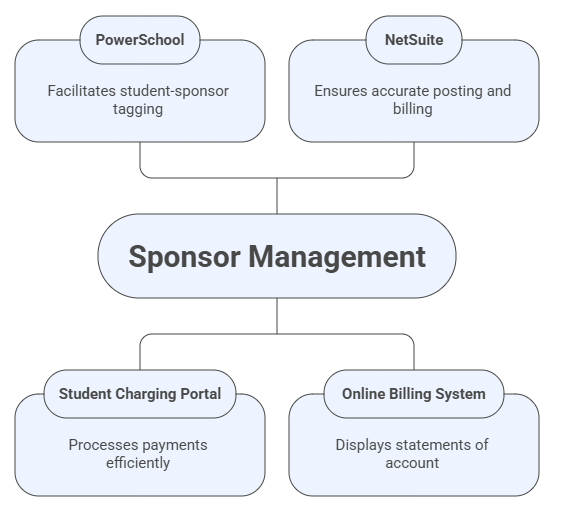
\includegraphics[width=300pt]{images/streamline.png}
                \caption{Streamlining Sponsor Management}
                \label{fig:Streamlining Sponsor Management}
    \end{center}
    \end{figure}
    
    As shown in Figure~\ref{fig:Streamlining Sponsor Management}, the proposed Sponsor Management layer is the common point of reference for PowerSchool, Student Charging Portal, NetSuite and Online Billing System. The figure is provided to illustrate the centralization of sponsor records and the rules for coverage of LoG before deciding on billings and sending to finance and statement systems.
    
    PowerSchool is used for sponsor tagging of students, NetSuite is the posting/billing ledger, the Sponsor Management layer holds all sponsor information and LoG rules, the Student Charging Portal is used for charge entry and coverage evaluation, and the Online Billing System publishes statements showing the final Bill-To and allocations.
    
    \subsection{Overview}
    
    This work resulted in a deployed pilot web application, at \url{http://ismsponsor.azurewebsites.net/}, where sponsors will be able to use self-service functions to manage their information (name, TIN, addresses, multiple contacts), obtain a list of LoG entries for each student per school year, and create or edit LoG entries via a guided modal form with status tracking.

        %Context Diagram
        \begin{figure}[H]
        \begin{center}
            \vspace{2ex}
            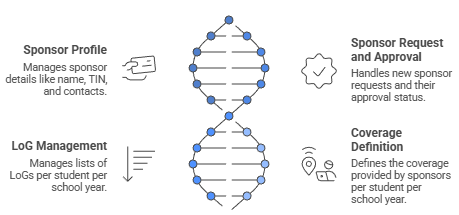
\includegraphics[width=400pt]{images/Application Features.png}
                \caption{Application Features}
                \label{fig:Application Features}
        \end{center}
        \end{figure}
    
    The main features of the pilot are described in Figure~\ref{fig:Application Features}, such as managing the sponsor profile, managing LoG, defining the coverage, handling sponsor requests, reporting support, etc. The figure is added to relate the introduced modules to the request to have a constant sponsor billing governance during operation. The system offers real-time calculation of preview for coverage on the Student Charging Portal and generates a decision with reason codes for operators.

    \subsection{Project Framework}
    
    Development was done in a DevOps manner with small tested releases to provide the ISM Sponsor Management and LoG Coverage Integration System. Requirements and integration mapping was validated initially, followed by development of features with automated builds, security validation, and end-to-end testing in \textbf{PowerSchool}, \textbf{NetSuite}, the \textbf{Student Charging Portal} and the \textbf{Online Billing System}. Deployment involved controlled deployments with monitoring, auditing and iterative improvements based on feedback.
  
    \begin{enumerate}
        \item \textbf{Plan.} Firstly, it was necessary to verify the end to end workflow and set the system boundaries. The requirements were identified for sponsor on boarding and approval, propagation of 18 sponsor master data, student sponsor tagging, creation of LoG per student per school year, and for billing LoG coverage synchronization. Admissions, Admin, Cashier and Sponsor had a role/permission matrix finalized. Integration contracts – all fields, Ids, timing, error handling, source of truth per record.
    
        \item \textbf{Design.} The solution was created as a role based web application consisting of different modules for Sponsor Profile, Sponsor Request and Approval, LoG Management and Coverage Management. The integration design defined the Sponsor master data to be published to each platform, the student Sponsor\_OrgName tagging process and how LoG coverage is represented for NetSuite enrollment profiles. Security features were woven into the design, comprising of server side security, audit logging and safe handling of attachments.
    
        \item \textbf{Continuous Integration and Build.} Development was in small steps in sync with the business workflow: Sponsor Onboarding and Approval, Integrations, LoG Workflows, Coverage to Billing Outputs. A CI pipeline was set up to perform unit tests, linting, dependency scanning and secret scanning on each and every change. Version built and traceable – any defect can be back-traced to a specific change set.
    
        \item \textbf{Test.} The testing process was carried out on a testing environment similar to the production environment as much as possible. Functional testing confirmed all workflows for each role, such as approvals, availability of sponsor list, syncing of student tags to the LoG creation/editing, and coverage completion. Data movement and correctness across all systems were tested and validated, while using controlled test data during integration testing. Security tests emphasized the isolation of roles, data access controls, attachment validation and audit log completeness. Testing was carried out for non-functional requirements for search, listings and modal workflows.
    
        \item \textbf{Release.} A release was made only when test evidence indicated that the entire sponsor to coverage process was stable. The release hardening involved configuration 19 checks, environment variables and secrets checks, as well as monitoring and logging checks. Release Notes and Rollback procedures were documented and go-live approvals were prepared from the system owners.
    
        \item \textbf{Deploy.} The deployment was done in a controlled fashion from staging to production. The smoke test after deploying confirmed that the sponsoring onboarding was available, the propagation of the sponsor list signals, the synchronization of the student tagging and the generation of LoG coverage was possible. Rollback was flagged as a tool that was immediately available in case of integrations and/or core workflows failing.
    
        \item \textbf{Operate and Monitor.} Once deployed, monitoring was focussed on application health, success rates of synchronisations and data consistency signals that showed mismatches across platforms. Audit logs were analysed for approvals and changes to records and alerts were spotted for tuning for integration failures that may impact billing readiness. Operational Run Books were created to address issues that occurred during sync failures, data mismatch, and user access problems.
    
        \item \textbf{Feedback and Improve.} Feedback from Admissions, Admin, Cashier and Sponsors has been gathered to understand the areas of pain and missing validations. Workflows were improved for support issues and monitoring trends for clarity, integration reliability and test coverage. Enhancements were identified which could be delivered from the same controlled pipeline with a continuous improvement without break on any billing critical processes.
    \end{enumerate}
   
    \subsection{Materials/Technologies Used}
    
    The deployed pilot leverages a Microsoft Azure-based technology stack to enable the secure development, structured validation and integration readiness between PowerSchool, NetSuite, the Student Charging Portal, and the Online Billing System.
    
    \begin{itemize}
        \item \textbf{Application Backend.} The back end was coded with . .NET ASP.The deployed pilot application on Azure App Service, secures and hosts REST API endpoints on NET Core. While testing and demonstrating the API endpoints for sponsor records, Letter of Guarantee management and coverage preview, the pilot used Swagger/OpenAPI documentation to expose, review, and validate them. Azure API Management, Azure Functions and Azure Key Vault were not included in the deployed pilot – they are only potential production-hardening components to consider if required.
    
        \item \textbf{Database Layer.} Sponsor records, contacts, Letters of Guarantee, coverage rules, the sync status and audit logs are stored on Azure SQL (MSSQL) as part of the database layer.
    
        \item \textbf{Web Front-end.} Front end for the web was designed as an ASP.Responsive and PWA compliant NET Core MVC interface with role specific pages for sponsor \& staff users. Pilot deployed with local credential authentication with Google OAuth readiness for future institutional credential authentication alignment.
    
        \item \textbf{Monitoring and Operations.} In the deployed pilot, monitoring was accomplished by looking at application logs, auditing, deployment checks and manual endpoint behavior validation. For future production hardening, expanded monitoring may be desired via Azure Monitor or Application Insights, but was not included in the scope of the pilot deployed.
    
        \item \textbf{Verification Aids.} Verification included Swagger/OpenAPI endpoint checks, staging smoke tests, repeatable validation scripts, security testing, performance testing and user acceptance testing to validate sponsor workflows, student tagging support, output of coverage for Letter of Guarantee, and role-based access behavior.
    \end{itemize}

    % FORMAT HIGHLIGHT: subsection heading
    % FORMAT HIGHLIGHT: subsubsection heading
    % FORMAT HIGHLIGHT: ampersands escaped for LaTeX compatibility
    % FORMAT HIGHLIGHT: LaTeX-safe conversion only; source wording retained
    
    \subsection{System Design}
    
    From a functional standpoint, the system entails sponsor master data management, Letter of Guarantee rule creation per sponsor \& per student, coverage evaluation for charge lines, audit logging of coverage decisions and same identifiers across sponsor, PowerSchool, Student Charging Portal, NetSuite and Online Billing System. Non-functional requirements are focused on security, using role-based access control and logging audits of actions performed; performance, ensuring that a common set of charge items can be covered in a timely fashion; and maintainability, with structured modules and documented endpoints.
    
    \begin{itemize}
        \item \subsubsection{Architecture Overview}
    
        The system is built to be a role-based web application in the \textbf{Microsoft Azure cloud} that centralizes sponsors' master data and Letter of Guarantee coverage rules, validates identifiers and outcomes, and prepares them for synchronization with \textbf{PowerSchool}, \textbf{NetSuite}, the \textbf{Student Charging Portal} and the \textbf{Online Billing System}. The solution is based on the use of an \textbf{ASP.NET Core} backend with business logic and REST API endpoints. The front end will be an \textbf{ASP.NET Core MVC} application with responsive, PWA-enabled interface for role-based access and \textbf{Azure SQL (MSSQL)} will be the primary data store. When the pilot is deployed, he or she exposes ASP.Azure App Service for hosting NET Core REST endpoints, and Swagger/OpenAPI for documenting, reviewing and validating endpoints as part of testing. Azure API Management, Azure Functions and Azure Key Vault were not included in the deployed pilot, and may be future components to be integrated to production and hardened.
    
        %Architecture overview
        \begin{figure}[H]
        \begin{center}
            \vspace{2ex}
            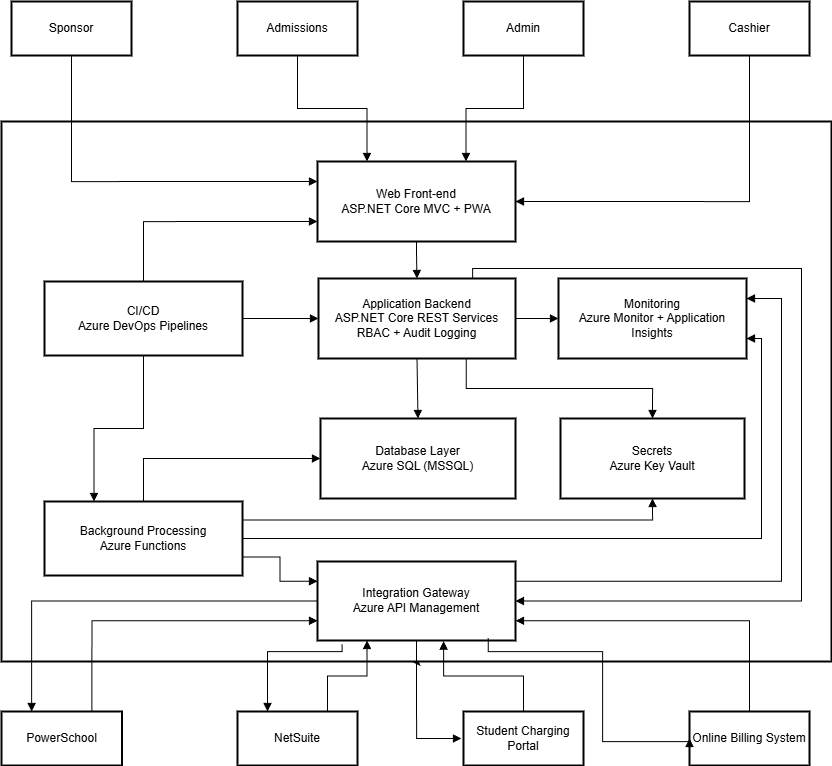
\includegraphics[width=0.88\linewidth]{images/Architecture overview.png}
            \caption{Architecture overview}
            \label{fig:Architecture overview}
        \end{center}
        \end{figure}

        \noindent Figure~\ref{fig:Architecture overview} details the Azure-based pilot architecture, including the role-based web interface, ASP.NET Core application layer, Azure SQL data store, monitoring services, and future API gateway path. The figure is included to show how the deployed pilot can support integration hardening without replacing ISM's existing systems.

        \item \subsubsection{Core Functional Services}
        
        The application offers 5 basic services. \textbf{Sponsor Master Data Management} stores sponsor \textbf{identity}, \textbf{TIN}, \textbf{Address} and \textbf{contact}s, and \textbf{provides controlled updates} and \textbf{approval} when necessary. LoG Rule Authoring can be done on sponsor and student level, allowing for differentiated coverage policies. \textbf{Coverage Evaluation} uses LoG rules to determine the covered/\textbf{bill-to} results for line items to be charged, including a quick preview path for frequently charged items. \textbf{Decision Auditing} captures all evaluation decision information including inputs, rule version, decision reason, user context and time/date of evaluation decision. Identifier Synchronization provides a consistent identifier for students and sponsors between \textbf{PowerSchool}, \textbf{SCP}, \textbf{NetSuite} and \textbf{OBS} to avoid mismatching coverage behavior.
     
        \item \subsubsection{Data Model and Persistence}
        
        Sponsor master records, contact records, LoG rule definitions, rule versions, effective date ranges, student-specific overrides, LoG instances per student per school year, and coverage results that are used by downstream billing are all stored in Azure SQL. audit log tables record each decision and important user action along with before/after values of changes. Sync status, last successful sync time, number of retries, and error information are stored in integration tracking tables to aid in operational visibility.
        
        %Sponsor Management ERD
        \begin{figure}[H]
            \centering
            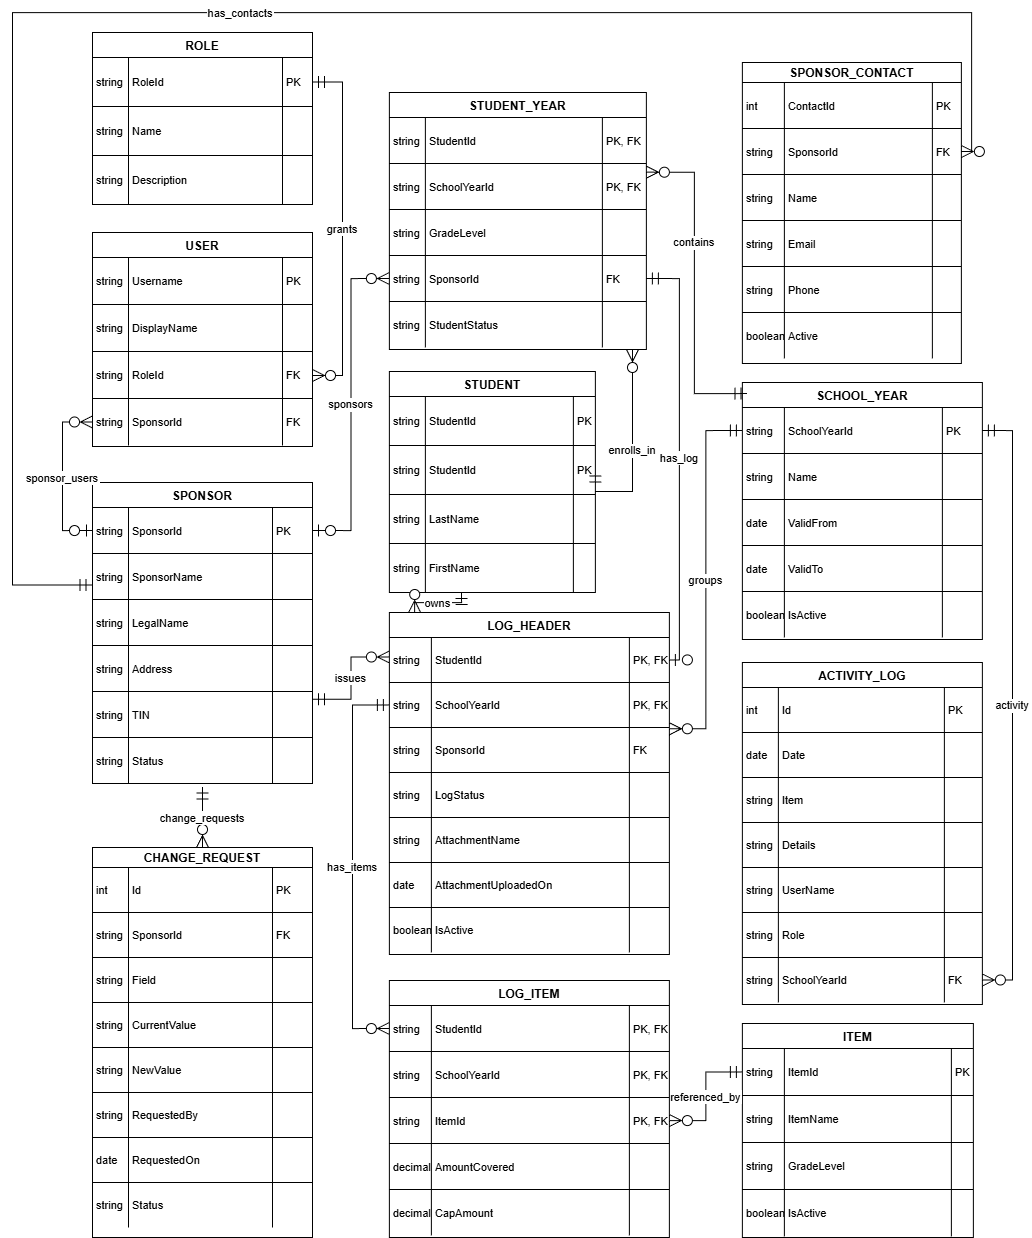
\includegraphics[height=0.72\textheight,keepaspectratio]{images/Proposal ERD.png}
            \caption{Sponsor Management ERD}
            \label{fig:Sponsor Management ERD}
        \end{figure}

        \noindent Figure~\ref{fig:Sponsor Management ERD} details the logical data model used by the pilot, including sponsors, contacts, users, roles, students, school years, LoG records, LoG items, charge requests, items, and activity logs. The figure is included to show how sponsor identity, coverage rules, and audit records are connected in the system database.
        
        \item \subsubsection{Coverage Computation and \textbf{Bill-To} Determination}
        
        System determines if a student is covered by the sponsor at charge line-level, based on deterministic rules based on the sponsor's LoG, and/or any student specific overrides. The result of each evaluation is a coverage classification and an authoritative Bill-To designation along with sponsor-parent allocation amounts and percentages and an auditable explanation of the reason code and rule version used for the evaluation. Student Identifier, Sponsor Identifier, School Year, Charge Item Code, Charge Category, Charge Amount, Charge Date, LoG effective date range, coverage caps or limits, exclusions, required documentation flags and student level overrides are inputs to the evaluation. The evaluation takes care of rule priority so that no two rules can have the same effect and result in an ambiguous or conflicting outcome.
        
        The coverage outcomes are defined as: (a) \textbf{Covered} – the sponsor is responsible for 100\% of the amount subject to the coverage caps and effective dates; (b) \textbf{Split} – the parent and sponsor are responsible for the amount subject to the coverage caps and effective dates following the rules defined herein; and (c) \textbf{Not Covered} – the parent is responsible for the amount subject to the coverage caps and effective dates.
        
        The explicit formulas are used to compute the allocation. In case of a cap based split, the system proceeds to calculate the following: SponsorCoveredAmount = min(ChargeAmount, RemainingCap) and ParentAmount = ChargeAmount - SponsorCoveredAmount. Percent allocations are calculated by dividing the amount covered by the Sponsor by the ChargeAmount (SponsorPercent) and the amount covered by the Parent by the ChargeAmount (ParentPercent). The monetary and percentage allocation to support downstream billing and reconciliation is recorded in the system.
        
        Bill-To is based on the calculated allocation. When SponsorPercent = 1.00, then Bill-To = Sponsor. SponsorPercent 0.00, Bill-To is Parent. If SponsorPercent is in the range 0.00 – 1.00, then Bill-To is Split and the explicit sponsor and parent allocations are propagated to downstream systems. For each decision a reason code and a rule version is persisted, so as to be traceable and auditable.
        
        \item \subsubsection{Integration Design}
        
        This is a sequence diagram of the real time interaction between systems in entering a charge. Student Charging Portal makes a Coverage API request to make a preview decision. The Coverage API queries the Sponsor Master for LoG and rule data, attempts to make a decision with allocations and audit data, and the portal pushes allocations to NetSuite and updates the Online Billing System (OBS) for statements to be displayed.
        
        %Integration Interaction Flow
        \begin{figure}[H]
            \centering
            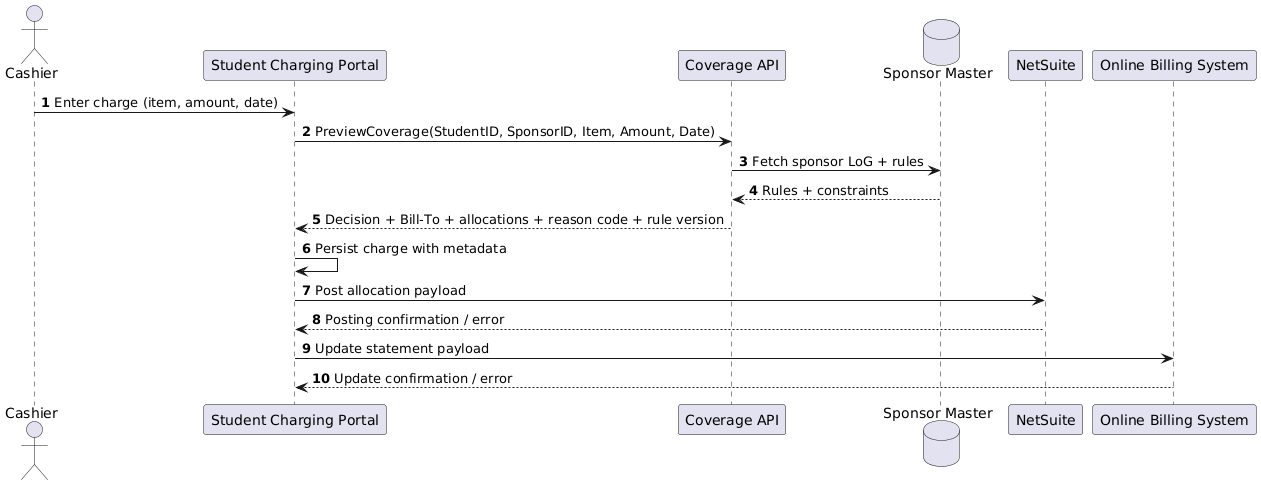
\includegraphics[width=0.98\linewidth]{images/integration flow.png}
            \caption{Integration Interaction Flow}
            \label{fig:Integration Interaction Flow}
        \end{figure}

        \noindent Figure~\ref{fig:Integration Interaction Flow} details the intended interaction between the Student Charging Portal, the coverage API, the Sponsor Master, NetSuite, and the Online Billing System. The figure is included to show how a charge entry can be evaluated once and then passed downstream with decision metadata and sponsor-parent allocation details.

        \item \subsubsection{Integration as the Core Implementation Component}
        
        The integration, as a core implementation component, is a structured approach that integrates materials and resources.
        
        An important aspect of the deployed pilot web application was the design of the integration that linked sponsor data, the coverage rules for LoG, the data about students, the decisions on charges, as well as outputs to the billing system across the existing ISM system landscape. The project was not designed to supplant or replace PowerSchool, NetSuite, the Student Charging Portal or the Online Billing System. It did, however, add a centralized Sponsor Master and coverage decision layer which could act as a common reference point for these systems.
        
        The integration part was crucial because the consistent identifiers and consistent interpretation of LoG provisions are necessary to sponsorship billing. The absence of a common integration layer means that names of sponsors, student records, charge categories, limits of expenditure (LoG) and assignments to a Bill-To can vary in meaning from one department to another and from one application to another. This problem was resolved by the deployed pilot who collected all the sponsor records, LoG records, coverage rules, audit records and downstream billing references into one application model.
        
        The pilot implementation confirmed the validity of the idea of integration via REST API endpoints, sponsor and LoG data structure, coverage preview response, audit decision records and synchronization-ready data structures. While integration with live production with PowerSchool, NetSuite and Online Billing System was not completely finished with the pilot scope, the application that was deployed provided the technical groundwork for future system to system exchange. This comprised of canonical sponsor identifiers, student references, LoG status fields, coverage-result structures, audit metadata and integration status endpoints.
        
        This integration-focused design allows for the project goal of delivering consistent, explainable and auditable coverage decisions with no requirement to replace ISM's enterprise systems. It also offers a pragmatic way to go forward with future production activities where API configuration, scheduled synchronization, error handling and reconciliation reports can be done and can be compared with live or staging institutional data. The supporting API and integration-readiness evidence is placed in \hyperref[app:integration-evidence]{Appendix A.6}.
     
        \setlength{\LTleft}{0pt}
        \setlength{\LTright}{\fill}
        \begin{longtable}{>{\raggedright\arraybackslash}p{0.22\linewidth}
                    >{\raggedright\arraybackslash}p{0.30\linewidth}
                    >{\raggedright\arraybackslash}p{0.40\linewidth}}
        \caption{Critical integration components of the deployed pilot web application}\label{table:critical-integration-components}\\
        \toprule
        \textbf{Integration component} & \textbf{Purpose} & \textbf{Pilot implementation evidence} \\
        \midrule
        \endfirsthead
        \caption[]{Critical integration components of the deployed pilot web application (continued)}\\
        \toprule
        \textbf{Integration component} & \textbf{Purpose} & \textbf{Pilot implementation evidence} \\
        \midrule
        \endhead
        \midrule
        \multicolumn{3}{r}{\textit{Continued on next page}}\\
        \endfoot
        \bottomrule
        \endlastfoot
        Sponsor Master & Provides the canonical sponsor reference used by staff and sponsor-facing workflows. & Sponsor CRUD, duplicate prevention, sponsor profile management, sponsor contacts, and SponsorID-based records. \\
                    LoG Management & Maintains sponsor coverage documents, effective dates, statuses, and coverage-related rules. & LoG list, create LoG workflow, activation status, coverage fields, and sponsor-facing LoG views. \\
                    Coverage Evaluation & Produces consistent coverage outcomes for charge-related decisions. & Coverage preview API, reason codes, \textbf{Bill-To} outcome, sponsor and parent allocation fields, and audit record generation. \\
                    Audit Trail & Records decision and activity evidence for traceability and review. & Audit decision endpoint, activity logs, timestamps, rule references, and user action records. \\
                    External System Readiness & Prepares the application for future PowerSchool, NetSuite, Student Charging Portal, and Online Billing System synchronization. & REST API structure, integration status endpoint, mapped identifiers, Azure deployment, and synchronization-ready data model. \\
        \end{longtable}
        
        Table~\ref{table:critical-integration-components} shows why integration was treated as a core implementation component. The table connects each integration function to specific pilot evidence, showing that the web application was not merely a sponsor portal but a foundation for consistent system-to-system sponsorship billing governance.
        \pagebreak
        
        \item \subsubsection{Per-Application Activity Diagram}
        
        \textbf{PowerSchool Activity (Student Record and Sponsor Tagging).} This activity diagram outlines the student identity and sponsor linkage for PowerSchool. Staff create or update student records, add a SponsorID or sponsorship indicator, validate sponsor association and sync the student-sponsor relationship to the Sponsor Master. If the student is not connected to a sponsor, the student is parent responsible by default.
                 
        %PS Activity
        \begin{figure}[H]
        \begin{center}
            \vspace{2ex}
            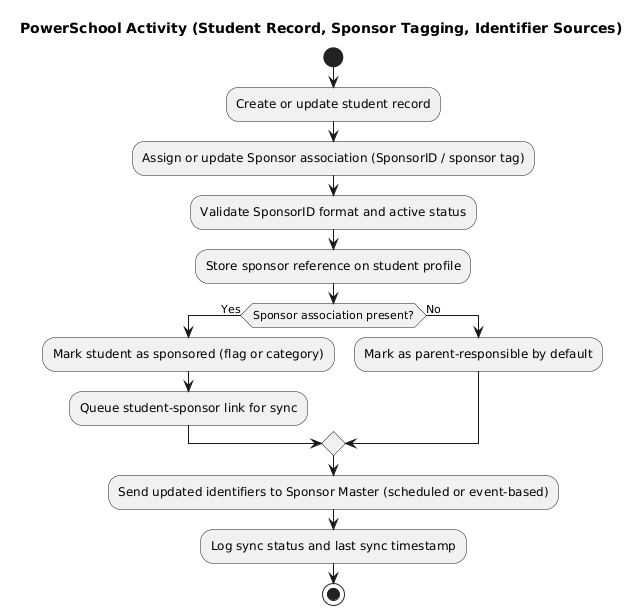
\includegraphics[width=350pt]{images/PS Activity.png}
            \caption{PowerSchool Activity}
            \label{fig:PowerSchool Activity}
        \end{center}
        \end{figure}

        \noindent Figure~\ref{fig:PowerSchool Activity} details the PowerSchool-related activity flow, where student identity and sponsor tagging provide the source linkage for sponsor-student association. The figure is included to show why consistent sponsor identifiers are needed before LoG coverage can be evaluated reliably.

        \textbf{Student Charging Portal Activity (Charge Entry and Coverage Preview).} This activity diagram illustrates the decisions that can be made at the point of charge entry which are supported by the Student Charging Portal. The user enters the charge information, asks for a coverage preview and obtains a coverage determination including allocations for sponsors and parents. The user agrees to this decision and the charge is posted with decision meta data to downstream systems. Otherwise, the user tweaks the inputs and preview runs again.
        
        %Student Charging Portal Activity
        \begin{figure}[H]
        \begin{center}
            \vspace{2ex}
            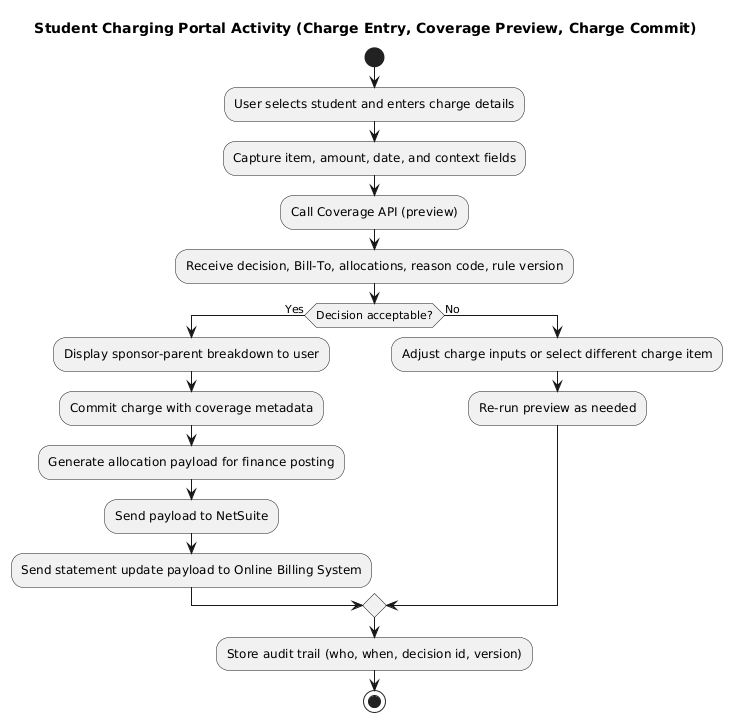
\includegraphics[width=350pt]{images/SCP Activity.png}
            \caption{Student Charging Portal Activity}
            \label{fig:Student Charging Portal Activity}
        \end{center}
        \end{figure}

        \noindent Figure~\ref{fig:Student Charging Portal Activity} details the charge-entry workflow in which the Student Charging Portal requests a coverage preview, receives a Bill-To decision, and commits the charge with decision metadata. The figure is included to show how manual LoG interpretation is replaced by repeatable rule-based validation at the point of charge entry.

        \textbf{NetSuite Activity (Allocation Posting and Receivables).} This activity diagram illustrates how NetSuite gets the allocation results and posts them as Receivables. NetSuite validates the payload, sets AR transaction lines for sponsor and parent portions, adds the decision metadata for Auditability and returns confirmation. Bad payloads are refused with error information and they are logged for debugging purposes.
        
        %NetSuite Activity
        \begin{figure}[H]
        \begin{center}
            \vspace{2ex}
            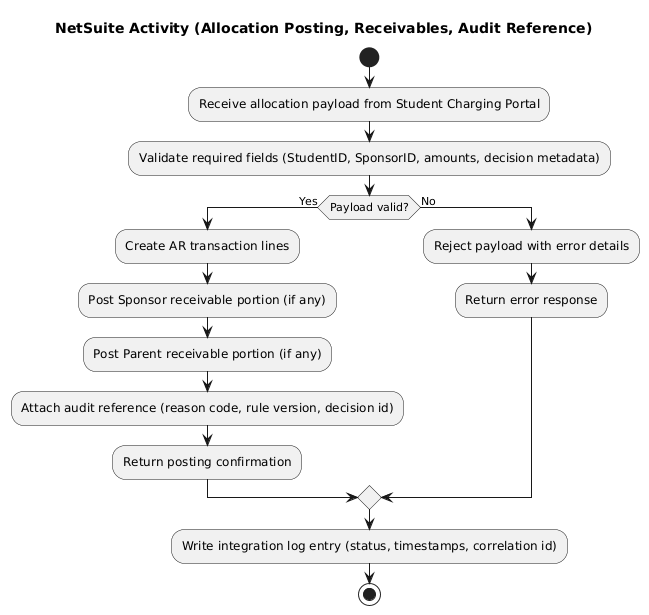
\includegraphics[width=350pt]{images/NetSuite Activity.png}
            \caption{NetSuite Activity}
            \label{fig:NetSuite Activity}
        \end{center}
        \end{figure}

        \noindent Figure~\ref{fig:NetSuite Activity} details how sponsor-parent allocation results would be validated and posted to NetSuite as receivable lines with audit references. The figure is included to show how the finance system can receive structured billing outcomes instead of manually interpreted charge assignments.

        \textbf{Online Billing System Activity (Statement Presentation).} This activity diagram depicts the Online Billing System's presentation of the billing outcome to the end users. It takes statement updates, validates the update, adds charge lines and sponsor-parent allocations and publishes an updated statement. It even includes the revision history and integration correlation identifiers for traceability.
       
        %Online Billing System Activity
        \begin{figure}[H]
        \begin{center}
            \vspace{2ex}
            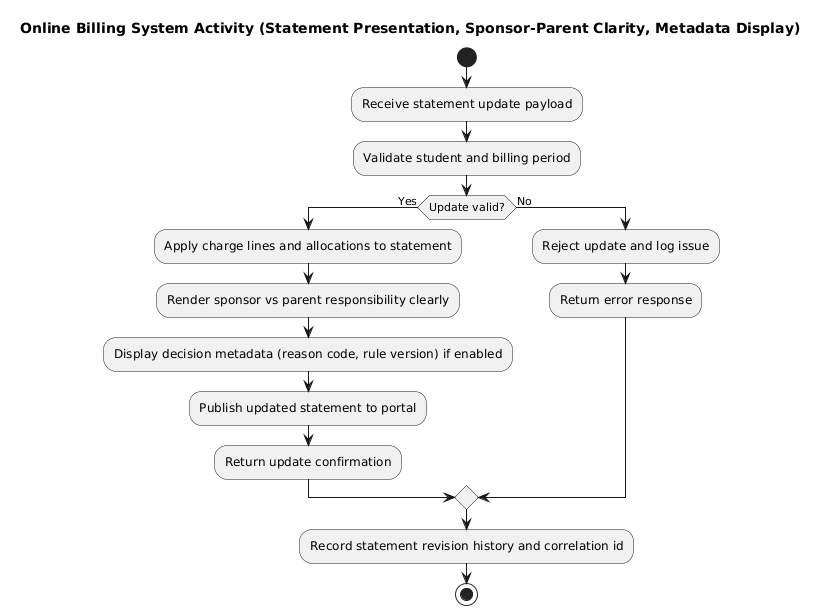
\includegraphics[width=350pt]{images/Online Billing System Activity.png}
            \caption{Online Billing System Activity}
            \label{fig:Online Billing System Activity}
        \end{center}
        \end{figure}

        \noindent Figure~\ref{fig:Online Billing System Activity} details how the Online Billing System would receive statement updates, apply charge lines and sponsor-parent allocations, publish updated statements, and retain revision history. The figure is included to show how the final billing view can reflect the same coverage decision produced during charge entry.

        \item \subsubsection{Cross-System Data Mapping and ERD Integration View}
        
        The integration view defines all the canonical student, sponsor, charge and allocation identifiers that are used to connect student, sponsor, charge and allocation records across systems. For those vendor schemas that have not been made available, or are proprietary, the manuscript supplies a logical view of the ERD integration showing emphasis on join keys, mapping fields and the direction of the synchronization.
       
        \setlength{\LTleft}{0pt}
        \setlength{\LTright}{\fill}
        Table~\ref{table:role-functions} lists the logical entities and key identifiers used to align sponsor, student, charge, and allocation data across the connected systems.
        
        \begin{longtable}{>{\raggedright\arraybackslash}p{0.18\linewidth}
                    >{\raggedright\arraybackslash}p{0.17\linewidth}
                    >{\raggedright\arraybackslash}p{0.21\linewidth}
                    >{\raggedright\arraybackslash}p{0.19\linewidth}
                    >{\raggedright\arraybackslash}p{0.17\linewidth}}
        \caption{Logical cross-system entity mapping and key identifiers}\label{table:role-functions}\\
        \toprule
        \textbf{Entity} & \textbf{PowerSchool (SIS)} & \textbf{Student Charging Portal} & \textbf{NetSuite (ERP)} & \textbf{Online Billing System} \\
        \midrule
        \endfirsthead
        \caption[]{Logical cross-system entity mapping and key identifiers (continued)}\\
        \toprule
        \textbf{Entity} & \textbf{PowerSchool (SIS)} & \textbf{Student Charging Portal} & \textbf{NetSuite (ERP)} & \textbf{Online Billing System} \\
        \midrule
        \endhead
        \midrule
        \multicolumn{5}{r}{\textit{Continued on next page}}\\
        \endfoot
        \bottomrule
        \endlastfoot
        \textbf{Student} & StudentID (authoritative) & StudentID (reference) & Customer/Student key (mapped) & Student account key (mapped) \\
                    \textbf{Sponsor} & Sponsor reference (if present) & SponsorID (reference) & CustomerID (mapped) & Sponsor account key (mapped) \\
                    \textbf{LoG} & Document reference (optional) & LoG record (reference) & Not stored as LoG (reference via audit id) & Displayed metadata (reference) \\
                    \textbf{Charge Line} & Optional fee definition & ChargeLineID (authoritative at entry) & Transaction/Invoice line key (mapped) & Statement line key (mapped) \\
                    \textbf{Allocation} & Not computed & Allocation fields (authoritative) & Accounting split fields (mapped) & Displayed split fields (mapped) \\
        \end{longtable}
                
        \item \subsubsection{Workflow Alignment}
        
        Sponsor onboarding starts with staff creation or submission of sponsor details and necessary documentation, and approval if applicable. Sponsor Identifiers are added and available in PowerSchool and downstream systems upon approval. Sponsor OrgName tagging in PowerSchool is the basis for student sponsor assignment, which is synced to NetSuite, OBS and SCP. LoG rules and/or student-level LoG coverage is defined and stored in the application and a decision to cover the charge line item is determined and recorded and synched to use for billing.

        %Context Diagram
        \begin{figure}[H]
        \begin{center}
            \vspace{2ex}
            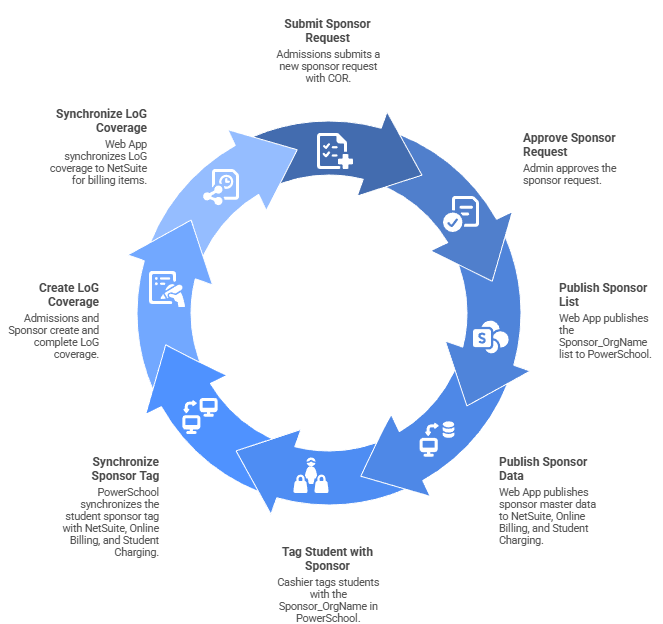
\includegraphics[width=400pt]{images/Context Diagram.png}
            \caption{Context Diagram}
            \label{fig:Context Diagram}
        \end{center}
        \end{figure}

        \noindent Figure~\ref{fig:Context Diagram} details the end-to-end context for sponsor requests, approvals, sponsor data publication, student tagging, LoG coverage synchronization, and billing outputs. The figure is included to show how the pilot sits between sponsor users, staff users, and the existing ISM system landscape.
    \end{itemize}
    \pagebreak
    
    \subsection{Implementation}
    
    The implementation involved three parallel threads:
    
    \begin{enumerate}
        \item Sponsor Master CRUD with contacts and addresses, name uniqueness checks against TIN and cross system-id.
        \item Create and Edit actions per student, with per student rules, caps and effective dates, status changes and notes.
        \item Functions in Coverage API that determine if a mock charge line qualifies for coverage and return decision along with reason codes and audit entries.
    \end{enumerate}
    
    The deployment was done with Azure DevOps pipelines and the deployment was Build to Test to Deploy to Dev to Manual Approval to Deploy to Pilot. De-identified records were used in the pilot data. The success measures were a decrease in manual checks, a decrease in reversals, and consistent Bill-To assignment at invoice creation.
 
    \subsection{User Interface Implementation}
    
    The User Interface of the \textbf{deployed pilot web application} was made to match with the current running Azure pilot application. It features a responsive role-based layout, a shared sign-in page, sidebar navigation that's role-aware, dashboard-specific views, and internal and sponsor-facing modules. The interface is responsive and PWA; but, it was not implemented as a full PWA as Installable offline behavior, service-worker caching, and a production web app manifest were not enabled in the pilot.
    
    The screenshots of the interface in this section have been inserted in the respective topics. This helps avoid the impression of a collection of visuals “displays” and enables the individual figure to validate the discussion in the body of the manuscript.
 
    \setlength{\LTleft}{0pt}
    \setlength{\LTright}{\fill}
    \begin{longtable}{>{\raggedright\arraybackslash}p{0.34\linewidth}
            >{\raggedright\arraybackslash}p{0.58\linewidth}}
    \caption{Interface topics and figure placement}\label{table:interface-visual-placement}\\
    \toprule
    \textbf{Interface topic} & \textbf{Figures placed in the manuscript} \\
    \midrule
    \endfirsthead
    \caption[]{Interface topics and figure placement (continued)}\\
    \toprule
    \textbf{Interface topic} & \textbf{Figures placed in the manuscript} \\
    \midrule
    \endhead
    \midrule
    \multicolumn{2}{r}{\textit{Continued on next page}}\\
    \endfoot
    \bottomrule
    \endlastfoot
    Login and responsive layout & Current ISM Sponsor Management sign-in page. \\
            Dashboard views & Administrator, Admissions, Cashier, and Sponsor dashboards. \\
            Sponsor and contact management & All Sponsors, Create Sponsor, All Contacts, Sponsor Profile, and Sponsor Contacts pages. \\
            Letters of Guarantee and coverage views & Internal LoG list, Create LoG page, sponsor-facing LoG page, and sponsor-facing Students page. \\
            Change requests and sponsor self-service & Sponsor Change Requests and Add New Contact pages. \\
            Reports and monitoring views & Administrator Reports and Sponsor Reports pages. \\
            Administrative settings and data maintenance & School Years, Student Management, Items Management, Role Management, and User Management pages. \\
    \end{longtable}

    Table~\ref{table:interface-visual-placement} shows how each screenshot supports a specific part of the interface discussion and confirms that the visual evidence is placed where the related topic is discussed.

    \setlength{\LTleft}{0pt}
    \setlength{\LTright}{\fill}
    \begin{longtable}{>{\raggedright\arraybackslash}p{0.20\linewidth}
            >{\raggedright\arraybackslash}p{0.72\linewidth}}
    \caption{Implemented role-based navigation in the deployed pilot web application}\label{table:implemented-role-navigation}\\
    \toprule
    \textbf{Role} & \textbf{Implemented navigation and accessible modules} \\
    \midrule
    \endfirsthead
    \caption[]{Implemented role-based navigation in the deployed pilot web application (continued)}\\
    \toprule
    \textbf{Role} & \textbf{Implemented navigation and accessible modules} \\
    \midrule
    \endhead
    \midrule
    \multicolumn{2}{r}{\textit{Continued on next page}}\\
    \endfoot
    \bottomrule
    \endlastfoot
    \textbf{Administrator} & Dashboard; All Sponsors; All Contacts; Letters of Guarantee; Reports; School Years; Students; Items; Roles; Users. Administrator dashboard actions also support sponsor review, LoG review queues, duplicate sponsor review, and sponsor record oversight. \\
            \textbf{Admissions} & Dashboard; Letters of Guarantee; Reports. Admissions workflows support sponsor review, draft LoG preparation, activation request, coverage-alignment checking, and coverage tracking. \\
            \textbf{Cashier} & Dashboard; All Sponsors; All Contacts; Letters of Guarantee; Reports. Cashier reporting supports reconciliation and coverage-decision review for billing verification. \\
            \textbf{Sponsor} & Dashboard; Letters of Guarantee; Students; Change Requests; Contacts; My Profile; Reports. Sponsor users can view their own records, submit profile-change requests, and review assigned LoGs and student coverage details. \\
    \end{longtable}

    Table~\ref{table:implemented-role-navigation} justifies the interface discussion because it reflects the current navigation structure shown in the captured application screens. It also confirms that staff-facing administration functions and sponsor-facing self-service functions are separated by role.
    \clearpage

    \subsubsection{Login and Responsive Layout}
    
    The application will start on the ISM Sponsor Management – Sign In page. The page offers an opportunity for staff users to sign in with an ISM Google account, and also offers username/password access for Sponsor Organization users. This is in support of the bi-authentication model that was tested during pilot validation. In order to provide a document of the actual entry point for the deployed pilot web application, Figure~\ref{fig:login-responsive-layout} is placed directly below this topic. It also highlights the distinction between staff readiness to sign in to Google and access via their sponsor's username and password, allowing for the role-based access model validated during testing.

    \begin{figure}[H]
        \centering
        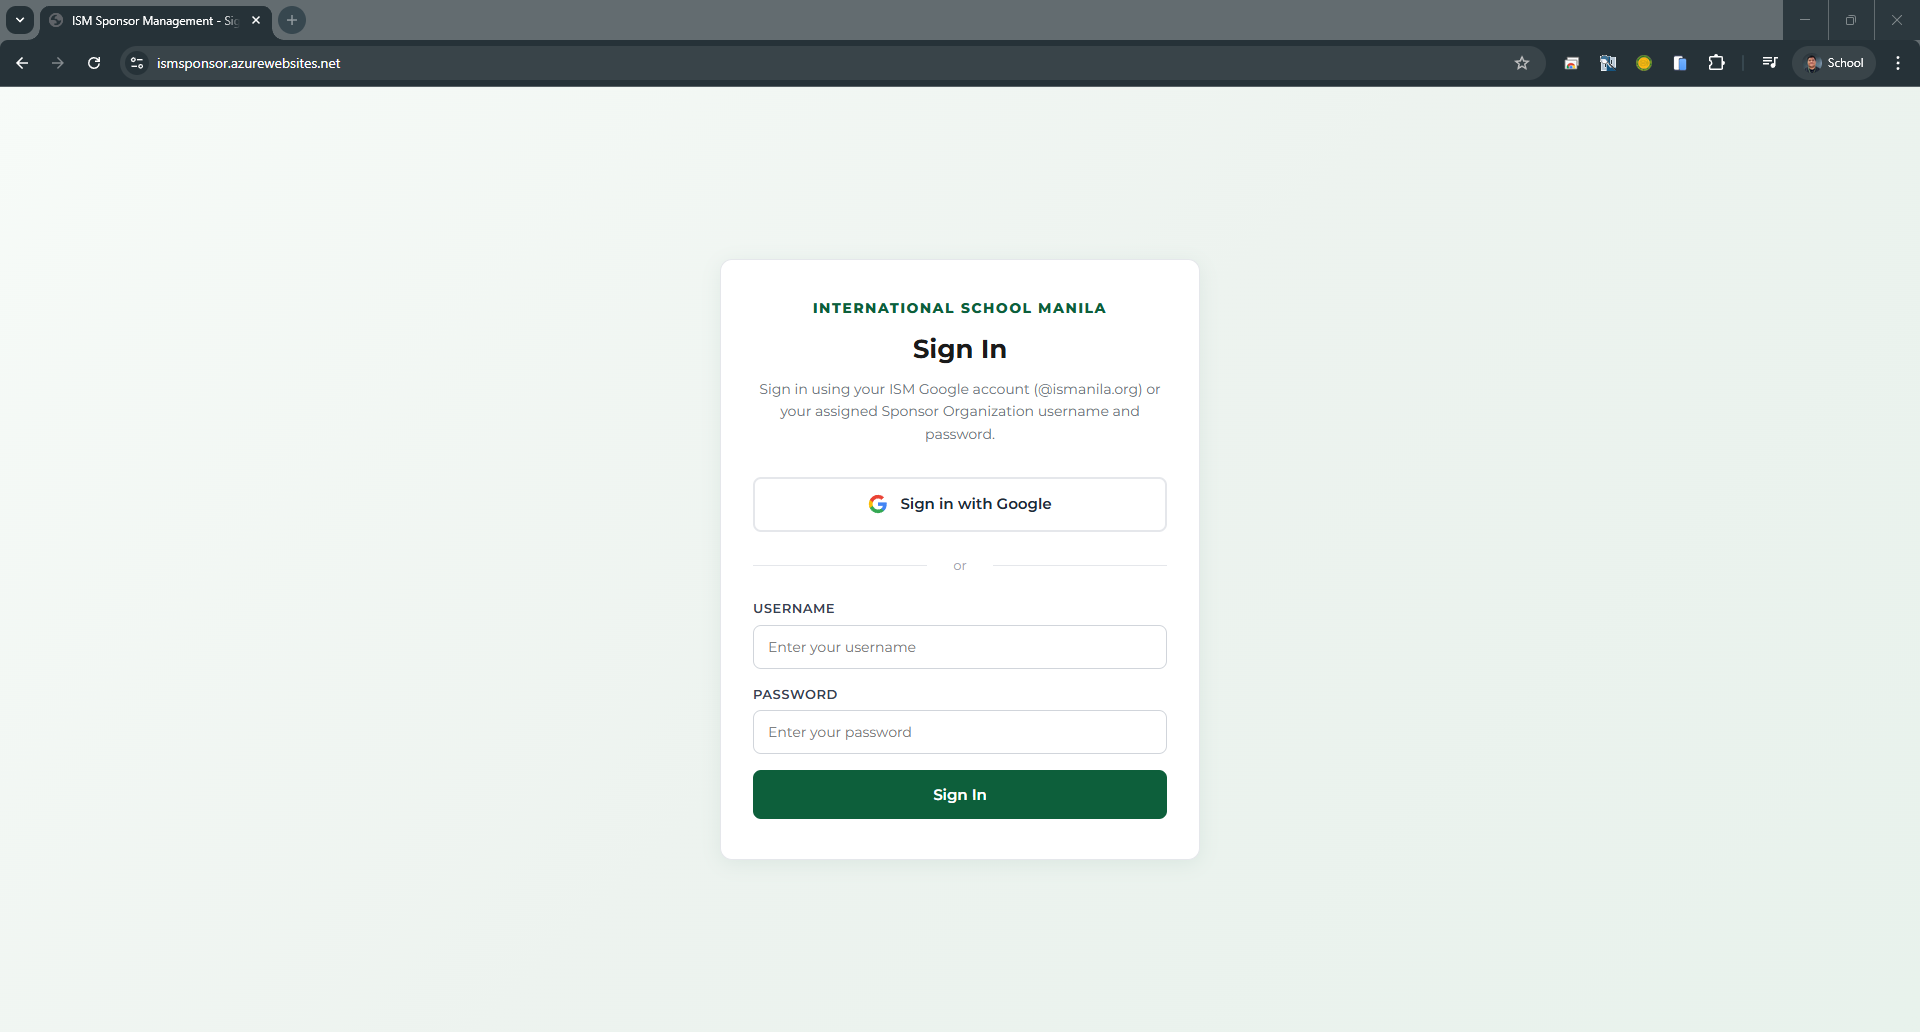
\includegraphics[width=0.90\linewidth]{images/current-interface/admin_login.png}
        \caption{Current ISM Sponsor Management sign-in page}
        \label{fig:current-login-page}
    \end{figure}

    \noindent Figure~\ref{fig:current-login-page} details the shared sign-in page used by internal staff and sponsor users in the deployed pilot. The figure is included to show the entry point for role-based access control, where authenticated users are routed to functions allowed by their assigned role.
    \clearpage

    \subsubsection{Dashboard Views}
    
    The deployed pilot makes available dashboard pages for the role. The indicators on the Administrator dashboard display the status of system-wide indicators of sponsor, LoG, change-request and user-management. Admissions and Cashier dashboards have more restricted views that are relevant to their work. Sponsor users will have their own portal dashboard to focus on their profile, students, Logs and change requests.

    \begin{figure}[H]
        \centering
        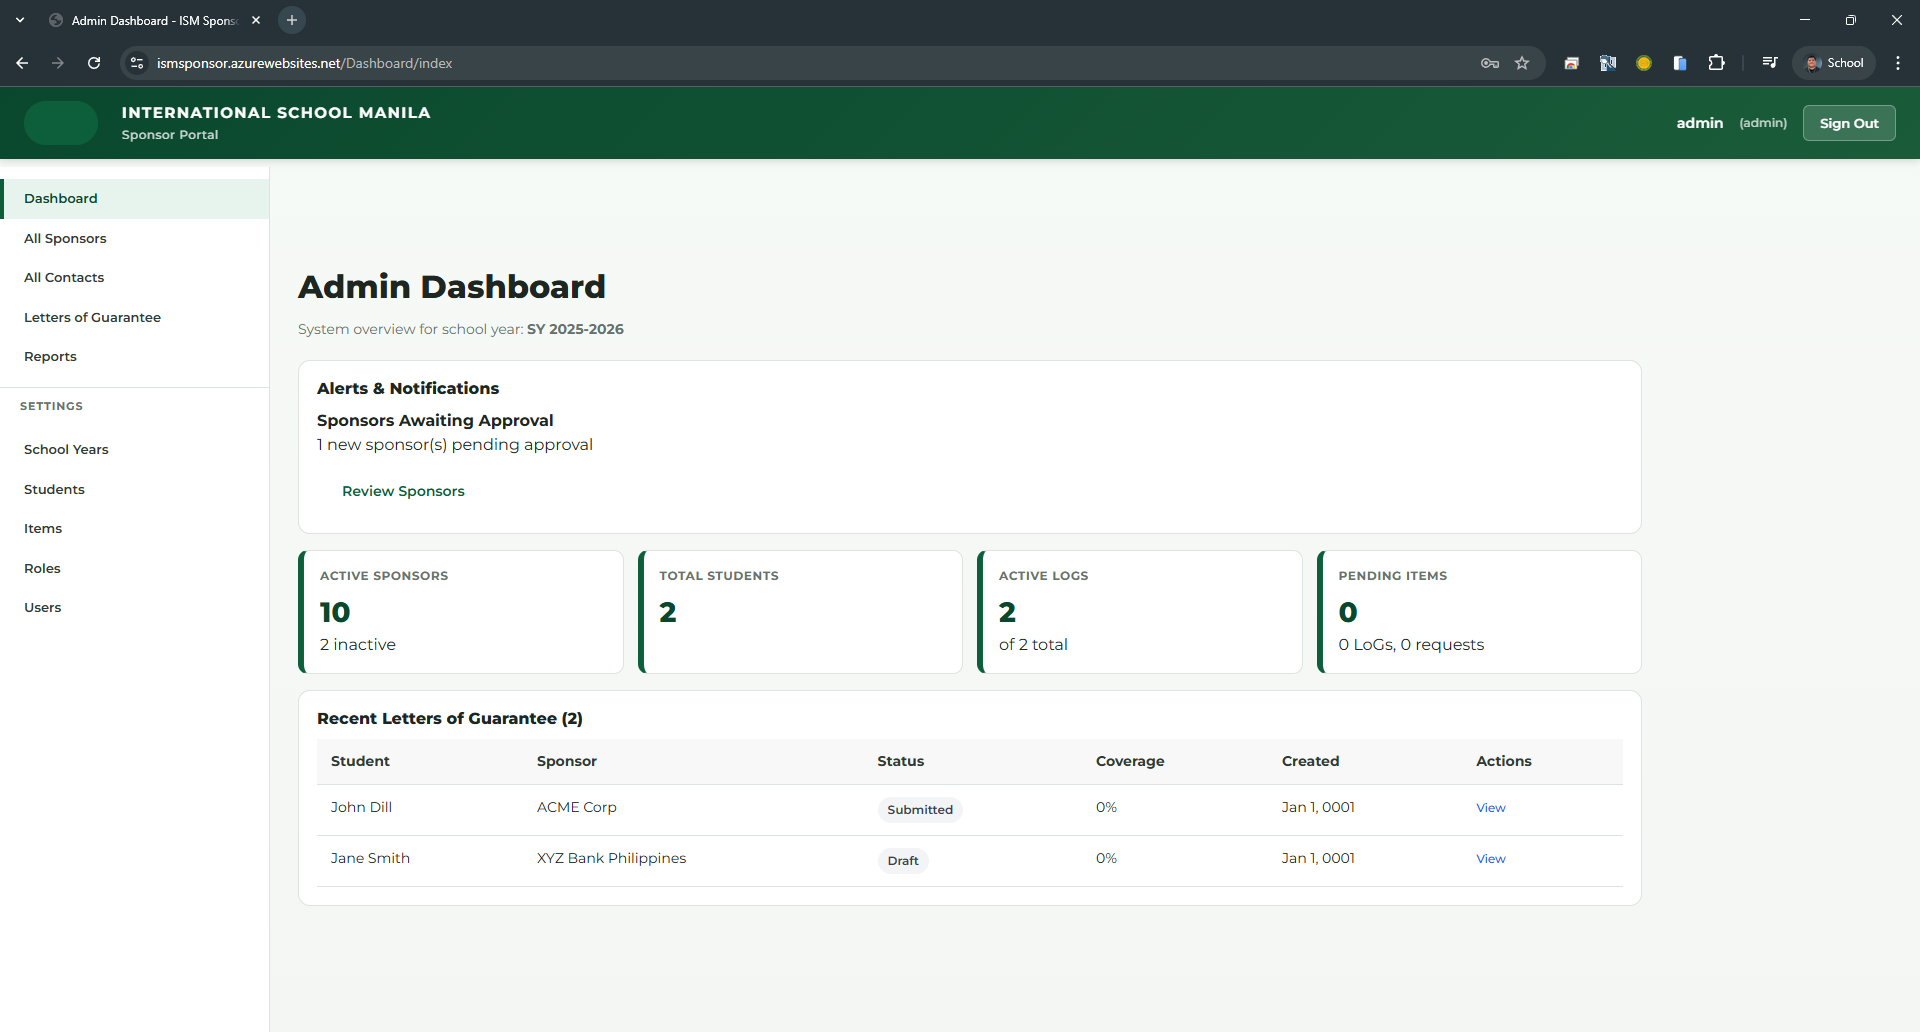
\includegraphics[width=0.90\linewidth]{images/current-interface/admin_dashboard.png}
        \caption{Administrator dashboard in the current deployed pilot web application}
        \label{fig:current-admin-dashboard}
    \end{figure}

    \noindent Figure~\ref{fig:current-admin-dashboard} details the Administrator dashboard, including summary counts, recent activity, and governance-oriented shortcuts for sponsor and LoG oversight. The figure is included to show how administrative users monitor the pilot and control records that affect sponsor billing decisions.

    \begin{figure}[H]
        \centering
        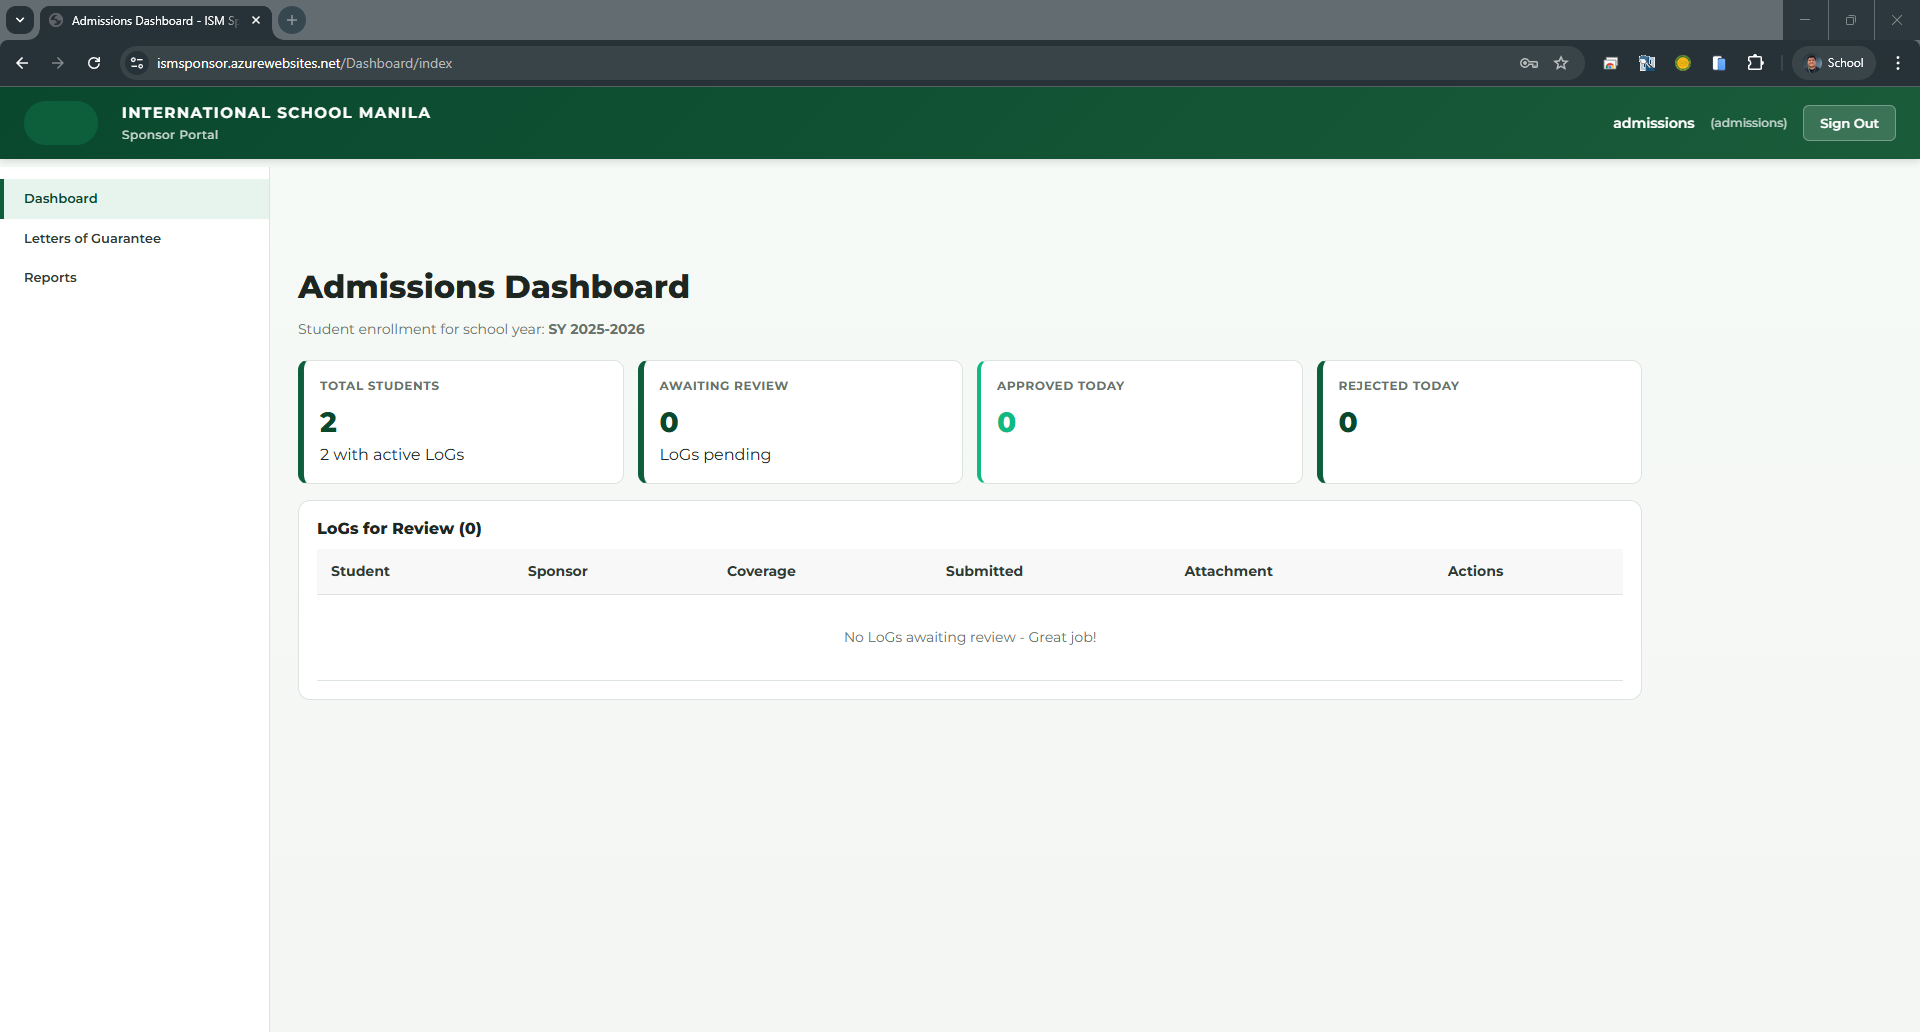
\includegraphics[width=0.90\linewidth]{images/current-interface/admissions_dashboard.png}
        \caption{Admissions dashboard in the current deployed pilot web application}
        \label{fig:current-admissions-dashboard}
    \end{figure}

    \noindent Figure~\ref{fig:current-admissions-dashboard} details the Admissions dashboard, which supports LoG preparation, sponsor review, and pending workflow monitoring. The figure is included to show how admissions-related users can prepare structured coverage information before administrative activation.
    \clearpage
    
    \begin{figure}[H]
        \centering
        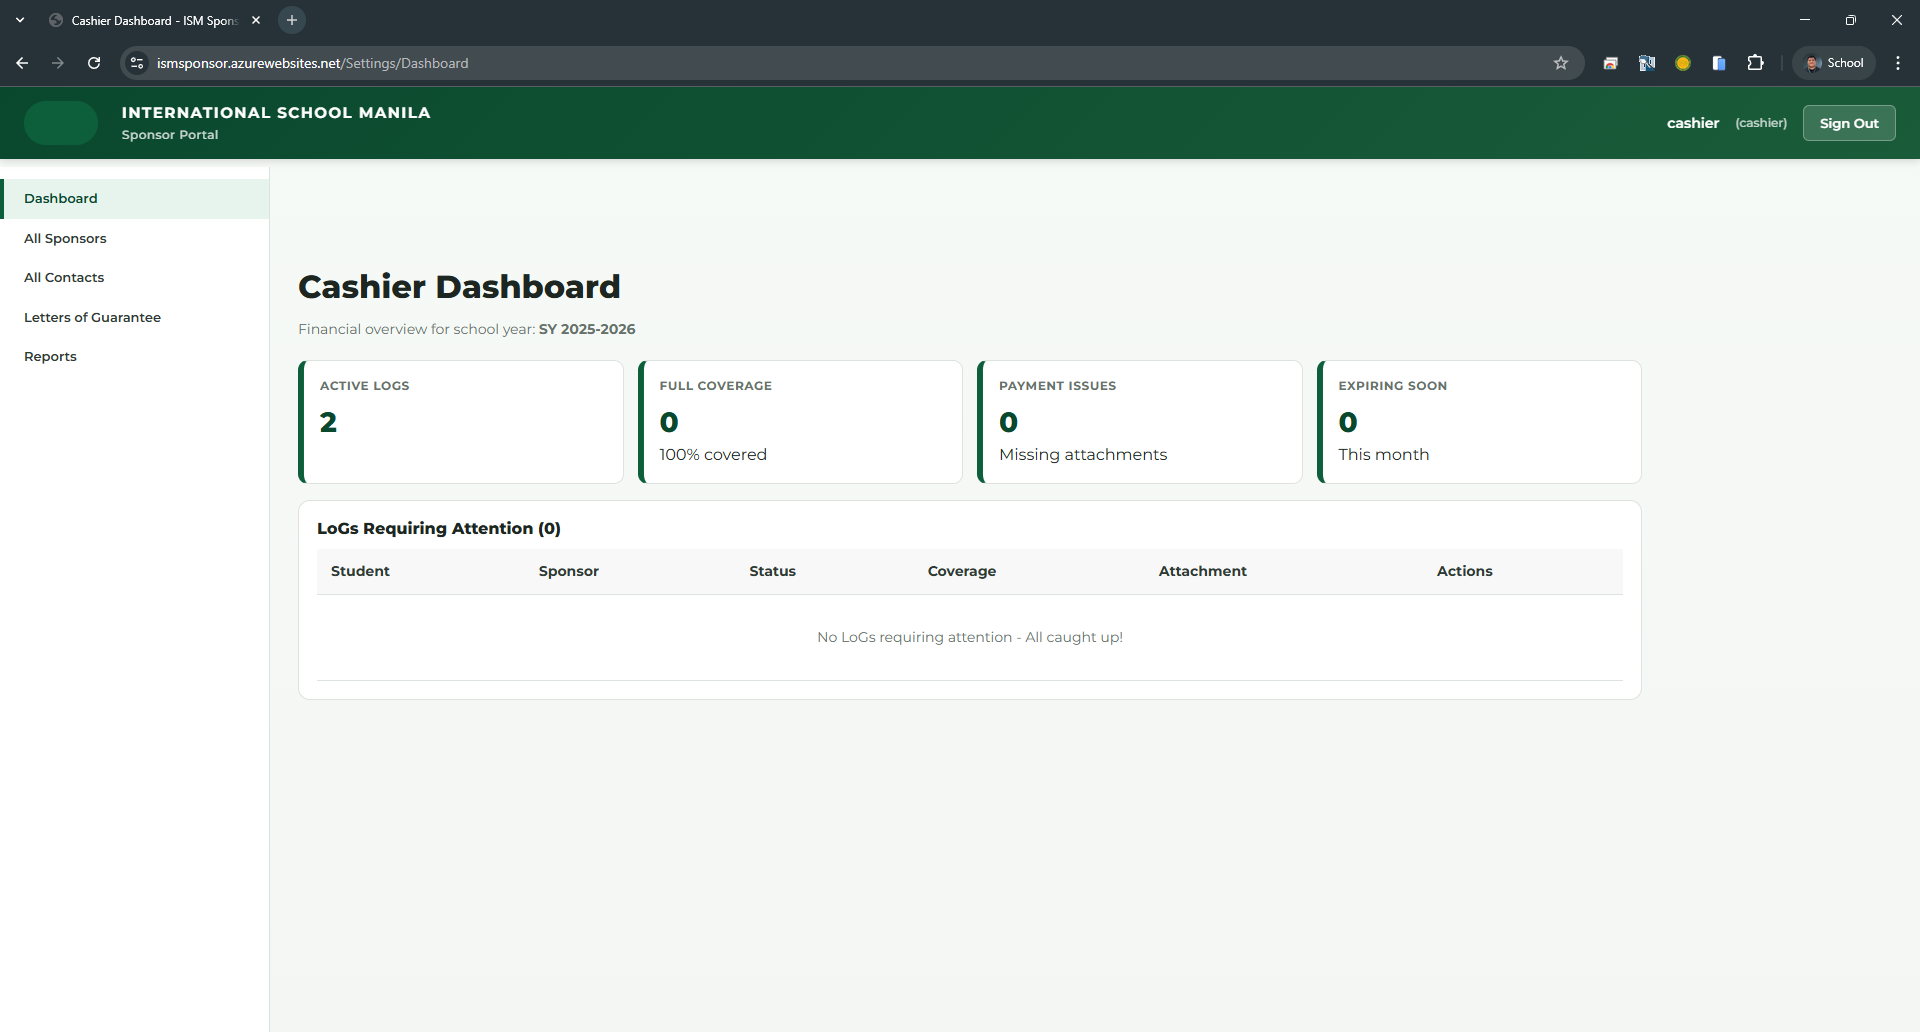
\includegraphics[width=0.90\linewidth]{images/current-interface/cashier_dashboard.png}
        \caption{Cashier dashboard in the current deployed pilot web application}
        \label{fig:current-cashier-dashboard}
    \end{figure}

    \noindent Figure~\ref{fig:current-cashier-dashboard} details the Cashier dashboard, which supports billing review, sponsor lookup, and reconciliation-related LoG monitoring. The figure is included to show how cashier users can verify sponsor and coverage information before or after charge processing.

    \begin{figure}[H]
        \centering
        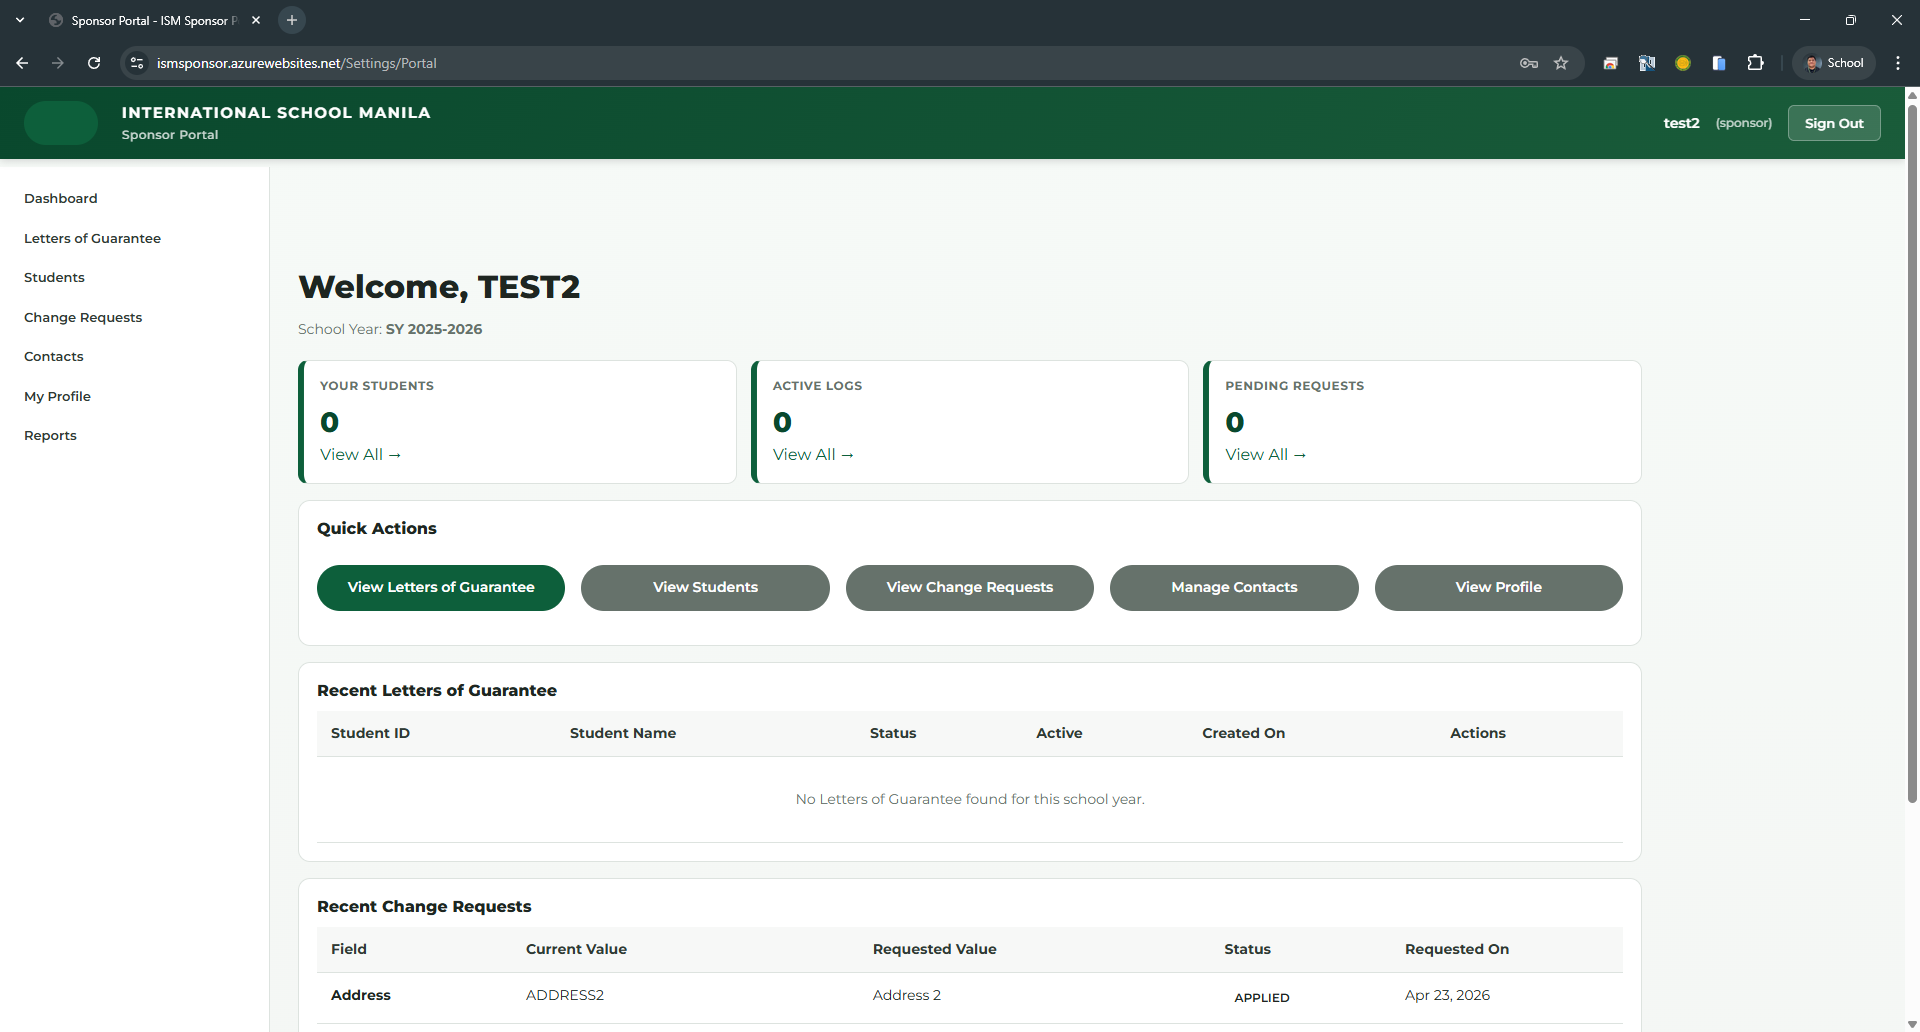
\includegraphics[width=0.90\linewidth]{images/current-interface/sponsor_dashboard.png}
        \caption{Sponsor dashboard in the current deployed pilot web application}
        \label{fig:current-sponsor-dashboard}
    \end{figure}

    \noindent Figure~\ref{fig:current-sponsor-dashboard} details the Sponsor dashboard, which limits visible information to the sponsor's own profile, students, LoGs, requests, and reports. The figure is included to show how the portal supports sponsor self-service while maintaining data boundaries.
    \clearpage

    \subsubsection{Sponsor and Contact Management}
    
    The management of the Sponsor is done via the All Sponsors module for authorized internal users, and via My Profile for Sponsor users. Administrator User roles can view, search and create sponsor records, whereas Sponsor User roles can only see their own profile and associated contact information.
    
    \begin{figure}[H]
        \centering
        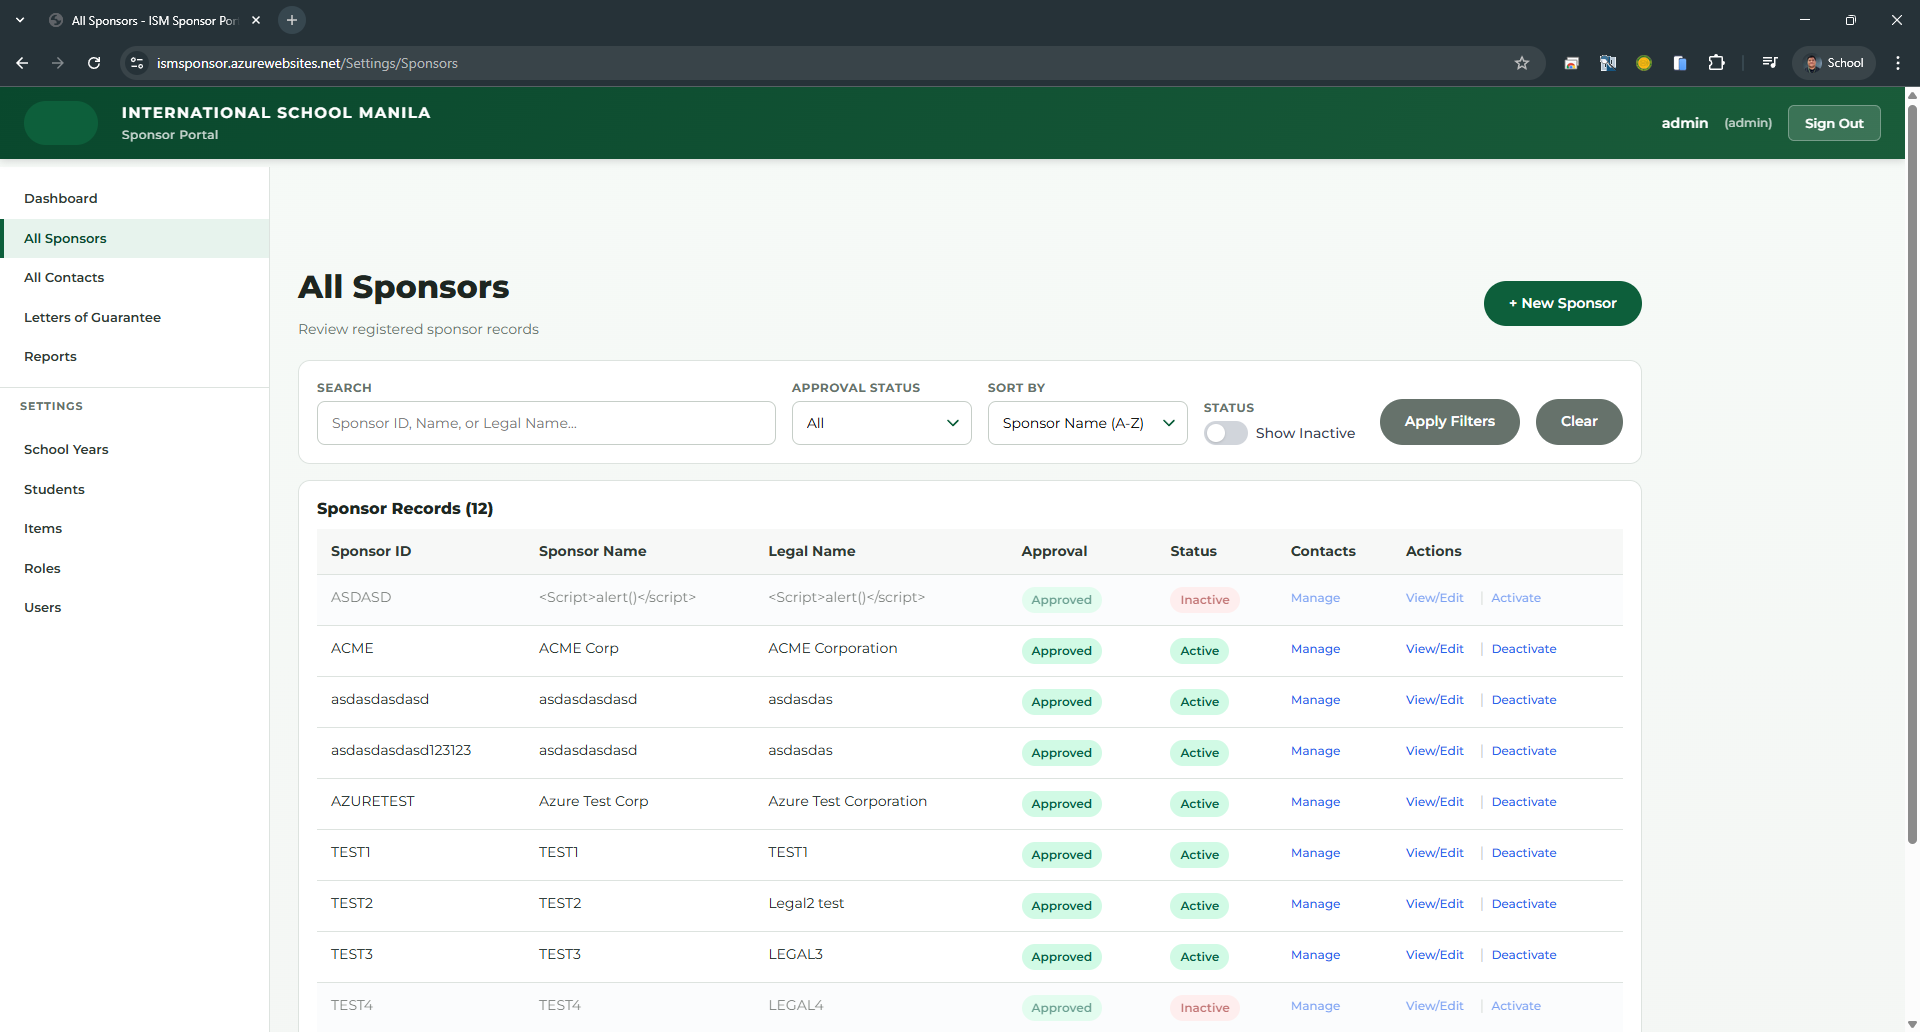
\includegraphics[width=0.90\linewidth]{images/current-interface/admin_all_sponsors.png}
        \caption{All Sponsors page for internal sponsor record management}
        \label{fig:current-all-sponsors}
    \end{figure}
    
    \noindent Figure~\ref{fig:current-all-sponsors} details the internal All Sponsors page, where staff can search, review, and maintain canonical sponsor records. The figure is included to show how the Sponsor Master reduces inconsistent sponsor naming and supports controlled sponsor record management.

    \begin{figure}[H]
        \centering
        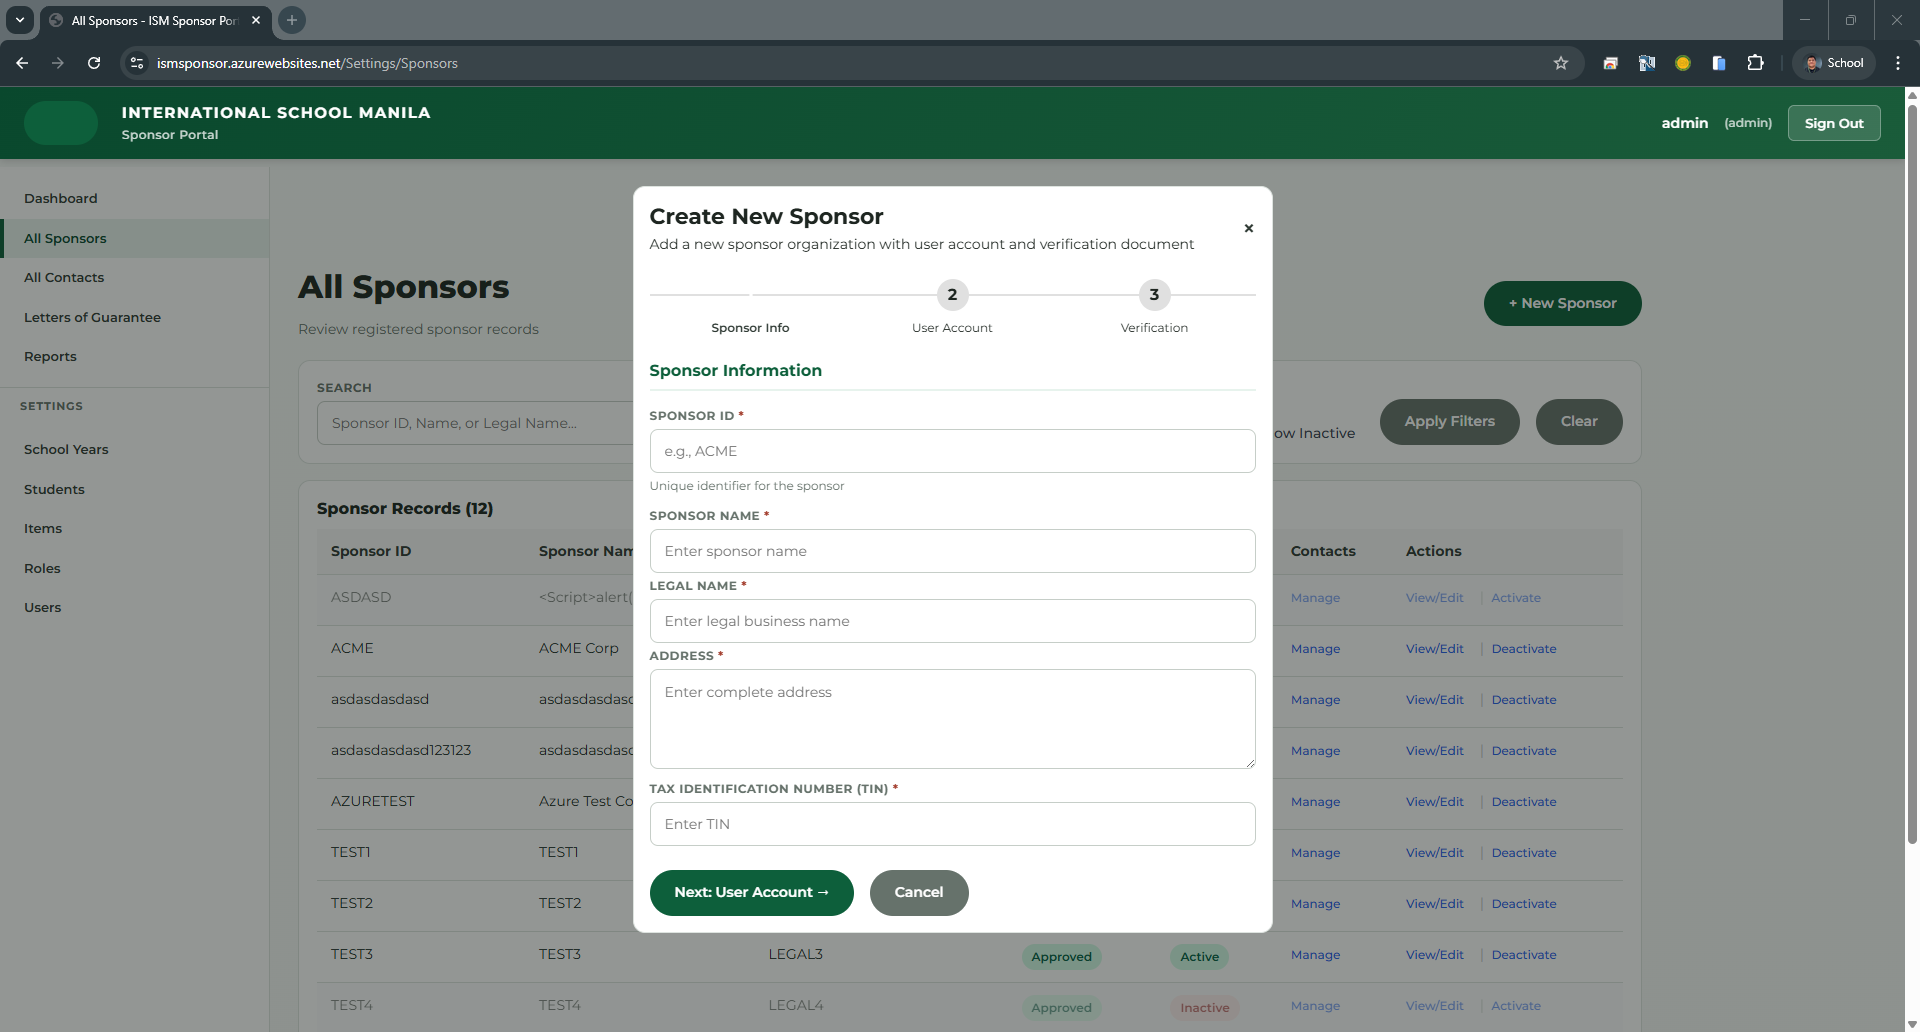
\includegraphics[width=0.90\linewidth]{images/current-interface/admin_create_sponsor.png}
        \caption{Create Sponsor page in the current Administrator interface}
        \label{fig:current-create-sponsor}
    \end{figure}

    \noindent Figure~\ref{fig:current-create-sponsor} details the Create Sponsor page, where administrator users enter sponsor identity, TIN, address, contact, and account-provisioning information. The figure is included to show how the pilot captures sponsor master data in structured fields rather than through informal notes or spreadsheets.
    \clearpage
    
    \begin{figure}[H]
        \centering
        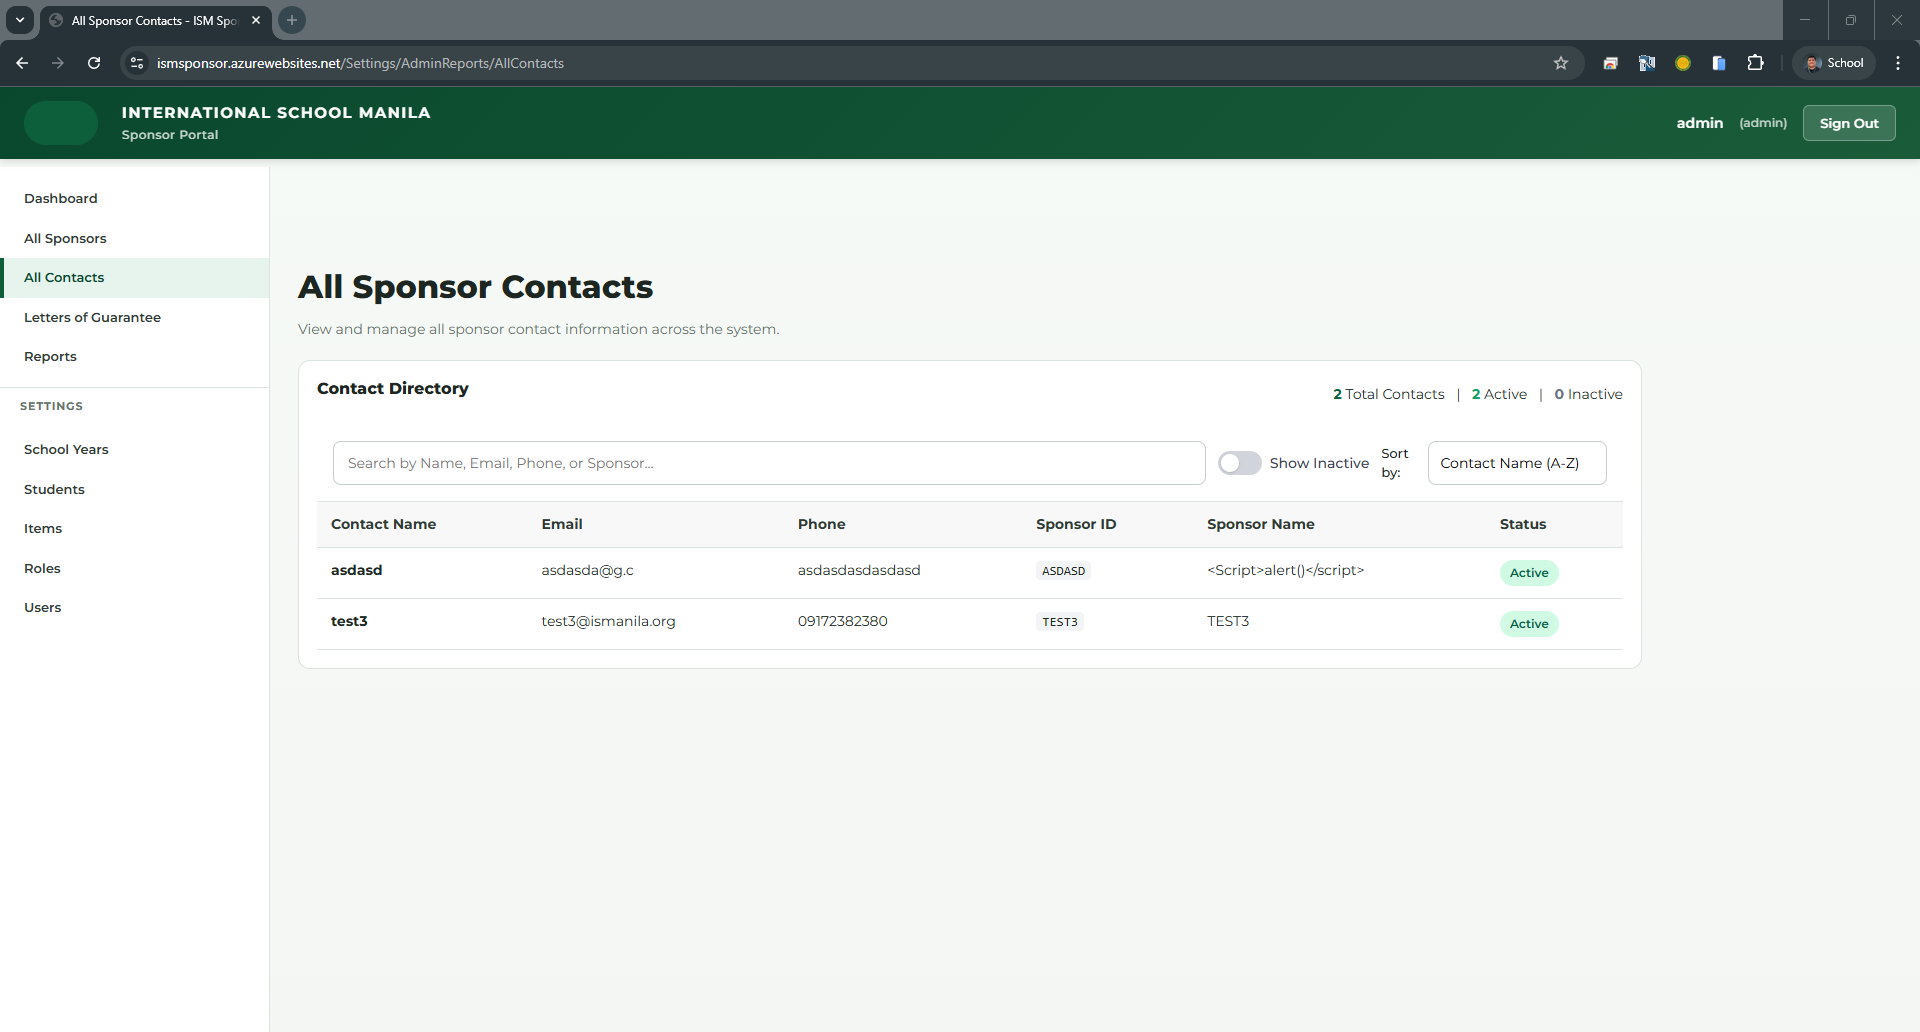
\includegraphics[width=0.90\linewidth]{images/current-interface/admin_all_contacts.png}
        \caption{All Contacts page for internal sponsor contact review}
        \label{fig:current-all-contacts}
    \end{figure}

    \noindent Figure~\ref{fig:current-all-contacts} details the All Contacts page used by staff to review sponsor contact records and related communication details. The figure is included to show how multiple sponsor contacts can be managed within the same controlled sponsor record.

    \begin{figure}[H]
        \centering
        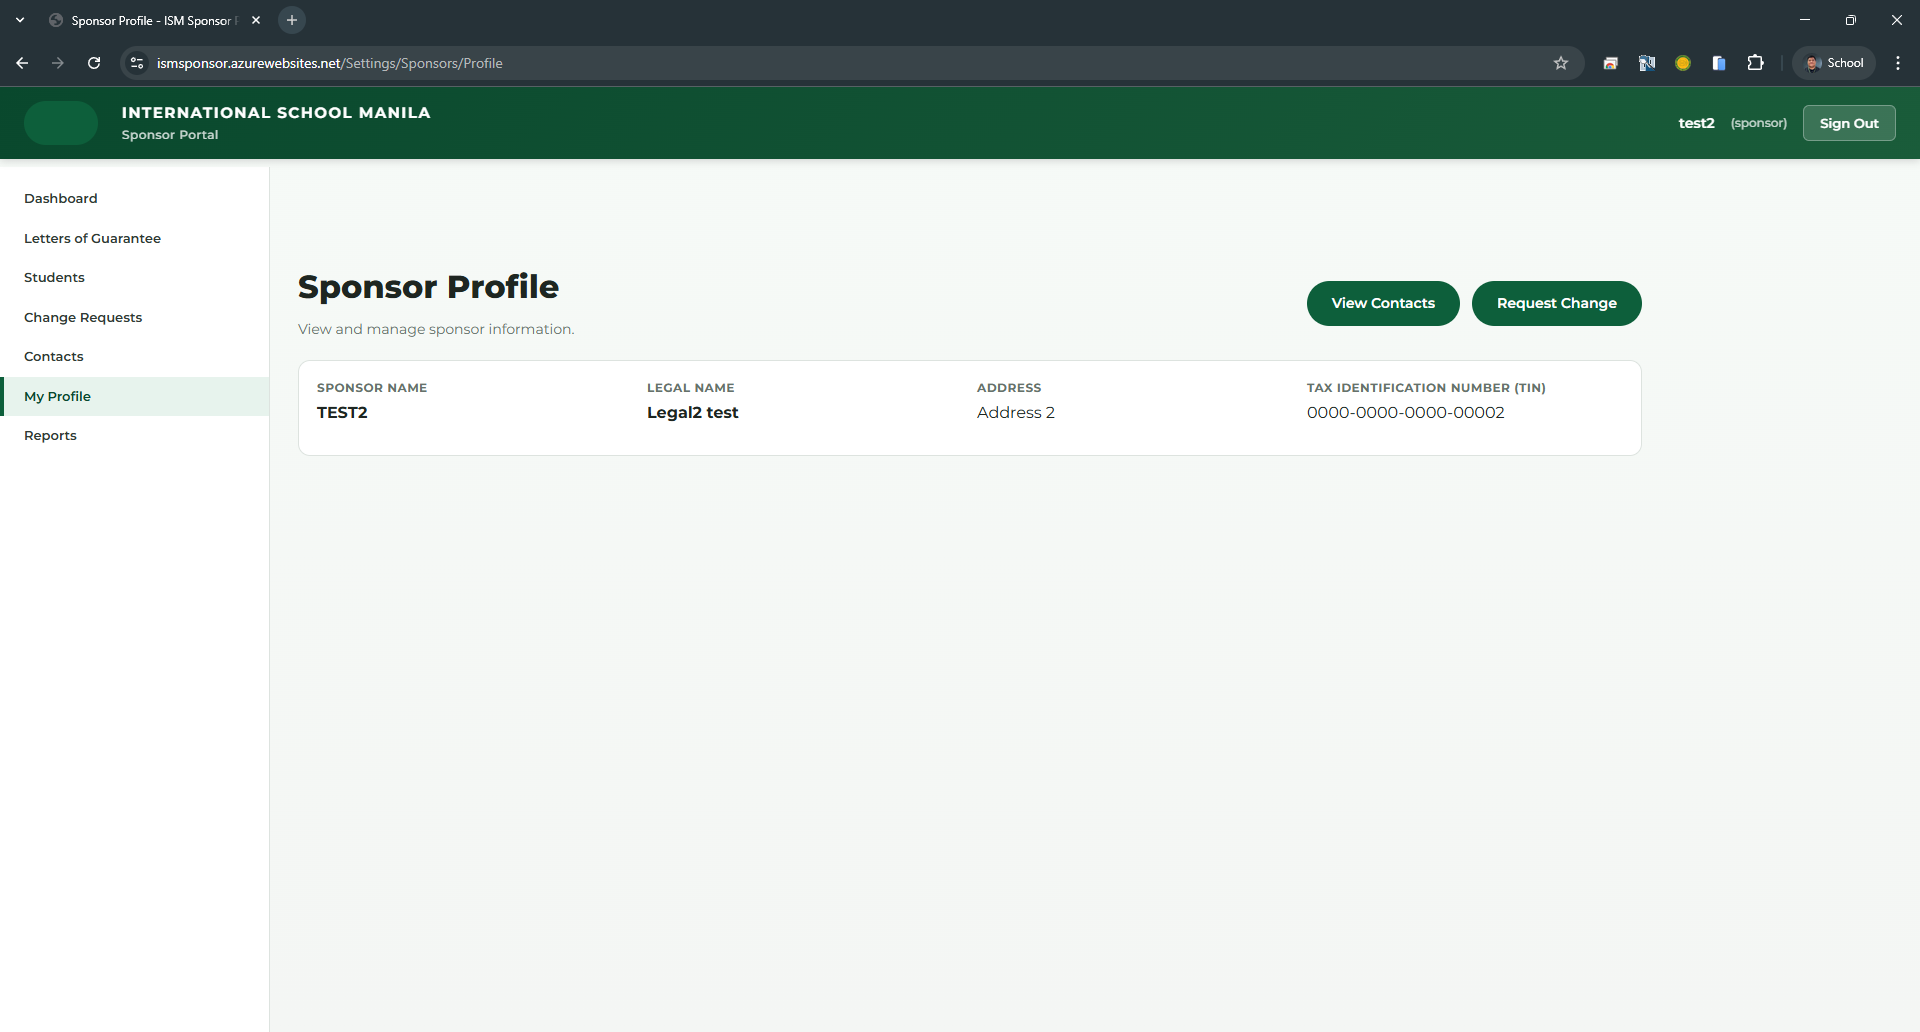
\includegraphics[width=0.90\linewidth]{images/current-interface/sponsor_profile.png}
        \caption{Sponsor profile page in the sponsor-facing portal}
        \label{fig:current-sponsor-profile}
    \end{figure}

    \noindent Figure~\ref{fig:current-sponsor-profile} details the sponsor-facing profile page, where external sponsor users can view their own approved organization information. The figure is included to show how sponsor self-service improves transparency while preventing direct uncontrolled edits to the Sponsor Master.

    \begin{figure}[H]
        \centering
        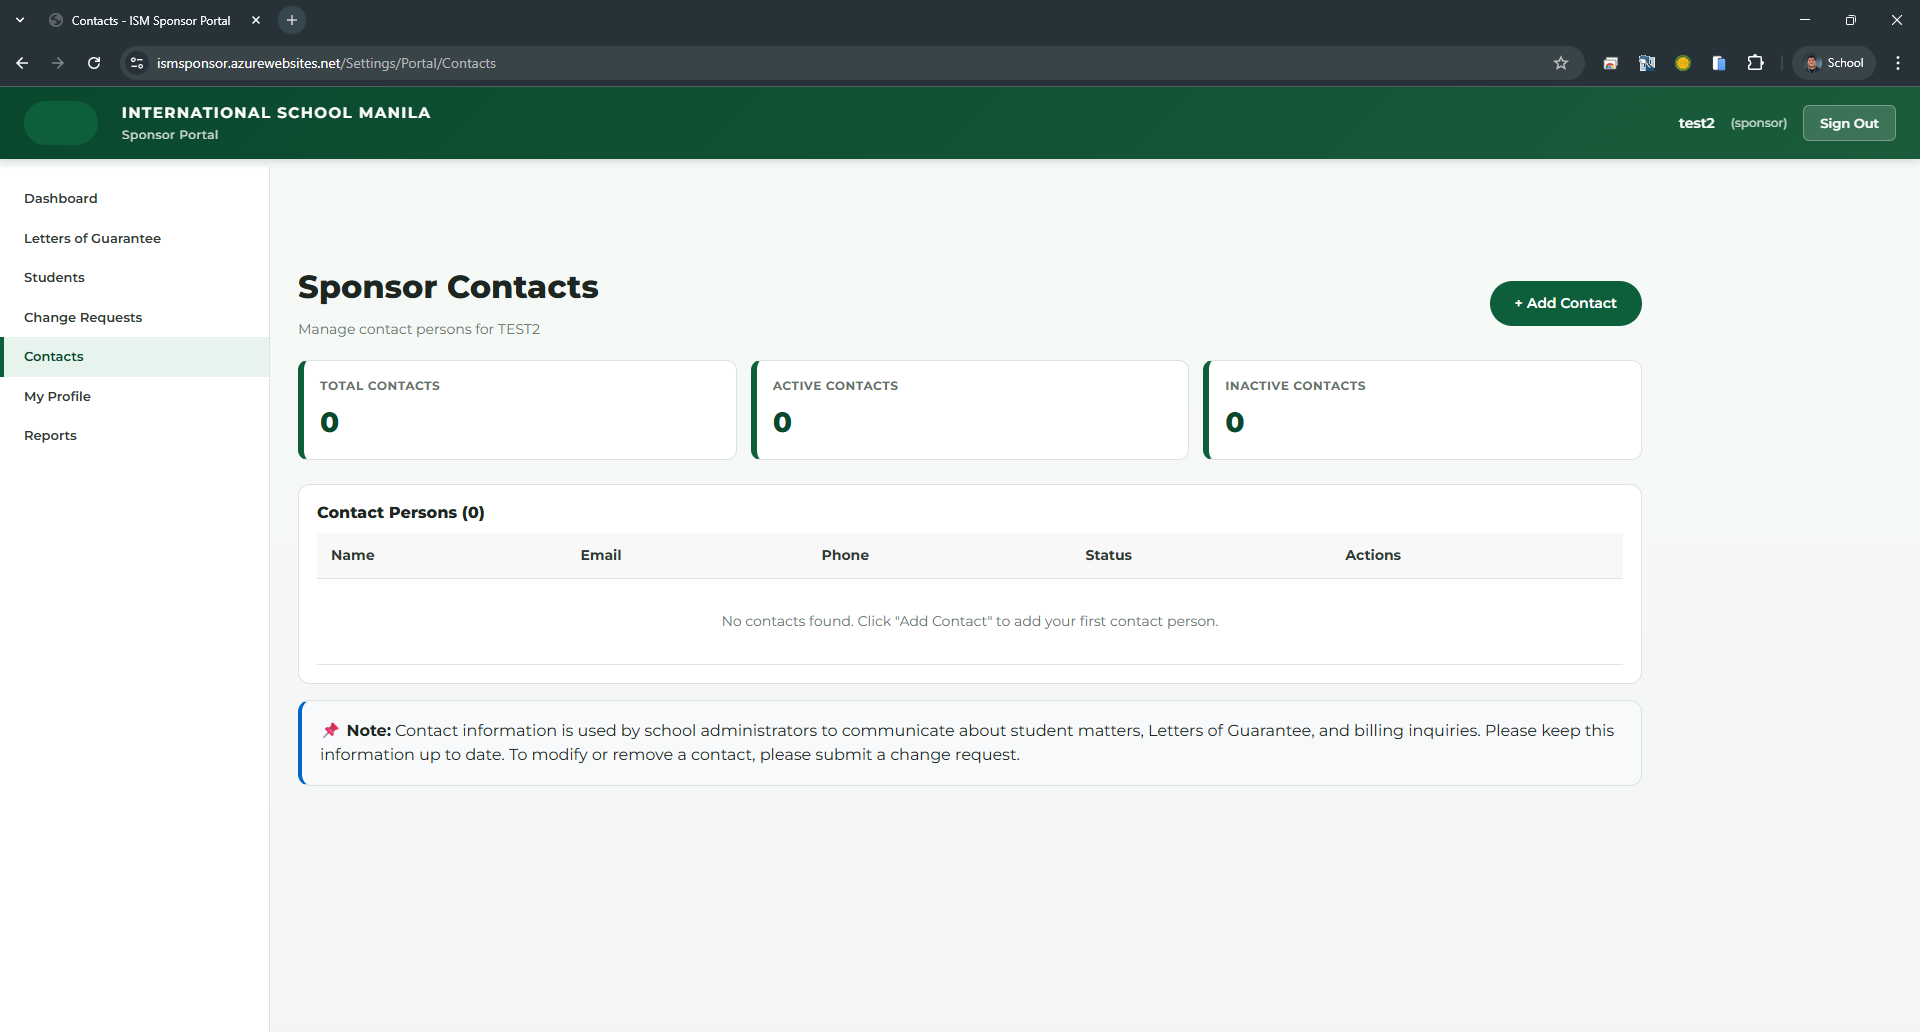
\includegraphics[width=0.90\linewidth]{images/current-interface/sponsor_contacts.png}
        \caption{Sponsor contacts page in the sponsor-facing portal}
        \label{fig:current-sponsor-contacts}
    \end{figure}

    \noindent Figure~\ref{fig:current-sponsor-contacts} details the sponsor-facing contacts page, where sponsor users can view contact information associated with their organization. The figure is included to show how external users can verify contact records without seeing records that belong to other sponsors.
    \clearpage

    \subsubsection{Letters of Guarantee and Coverage Views}
    
    Letters of Guarantee are put in place via internal and sponsor facing views. The Letters of Guarantee page is for internal users to view LoG records, develop LoGs, manage LoG coverage rules and verify LoG information. The sponsor user can see the assigned Letters of Guarantee from the sponsor portal but only in their records.

    \begin{figure}[H]
        \centering
        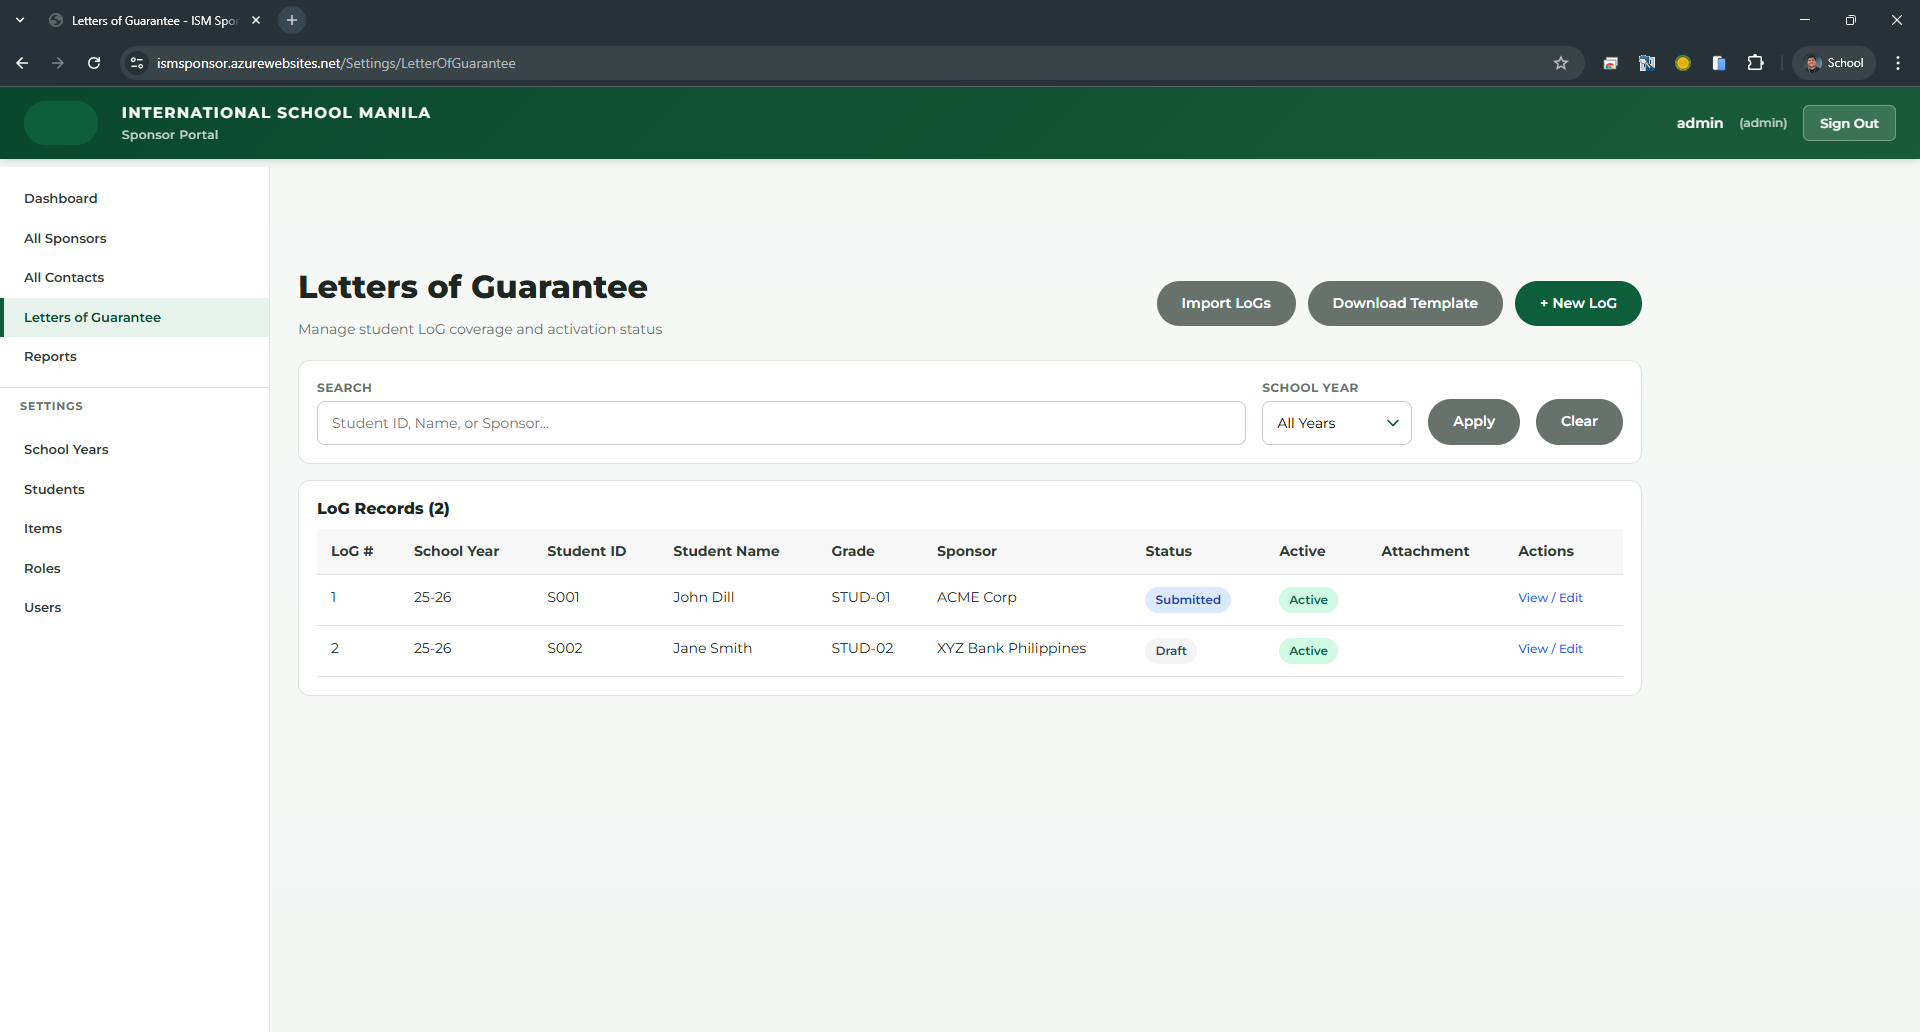
\includegraphics[width=0.90\linewidth]{images/current-interface/admin_log_list.png}
        \caption{Letters of Guarantee page for internal users}
        \label{fig:current-log-list}
    \end{figure}

    \noindent Figure~\ref{fig:current-log-list} details the internal Letters of Guarantee list used by staff to review LoG records, status values, attachments, and coverage actions. The figure is included to show how LoG records are made visible as structured workflow items rather than separate manually interpreted documents.

    \begin{figure}[H]
        \centering
        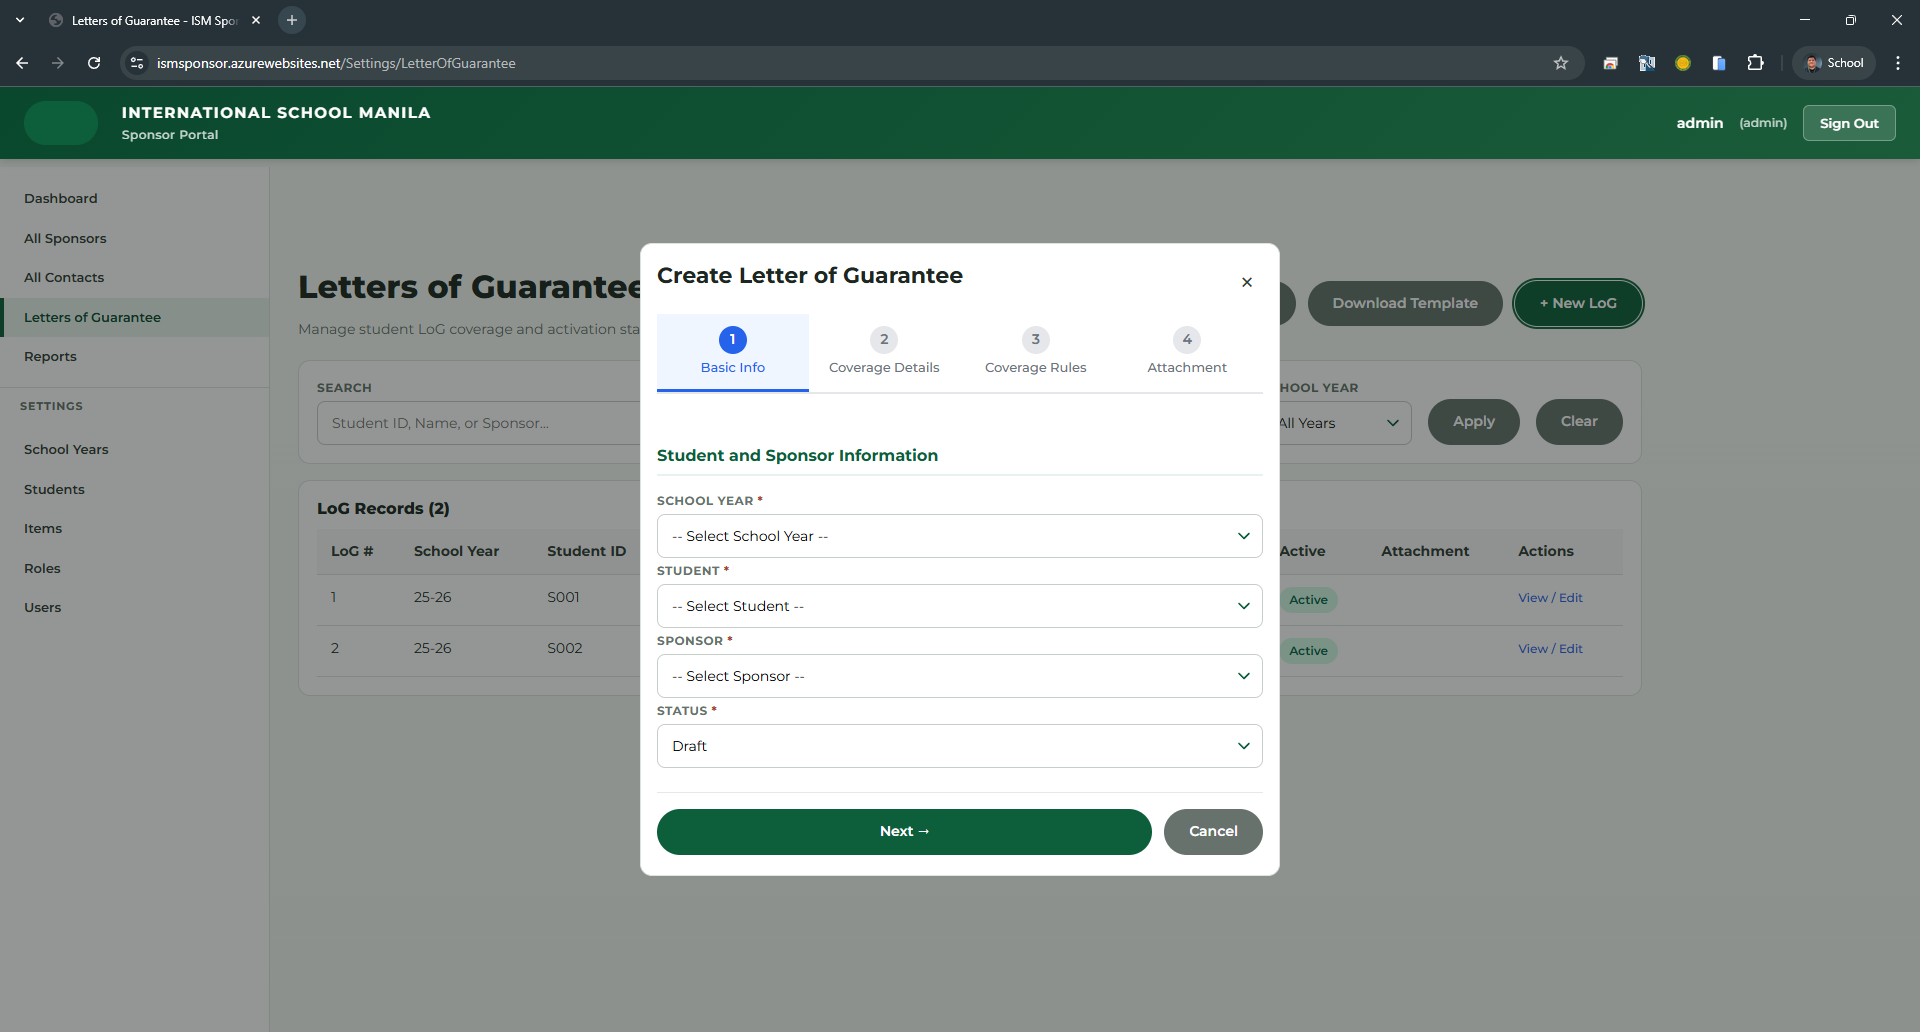
\includegraphics[width=0.90\linewidth]{images/current-interface/admin_create_log.png}
        \caption{Create Letter of Guarantee page with coverage-related fields}
        \label{fig:current-create-log}
    \end{figure}

    \noindent Figure~\ref{fig:current-create-log} details the LoG creation form, where staff define student, sponsor, school year, effective dates, status, and coverage-related fields. The figure is included to show how LoG content is converted into rule-ready data for later coverage evaluation.

    \begin{figure}[H]
        \centering
        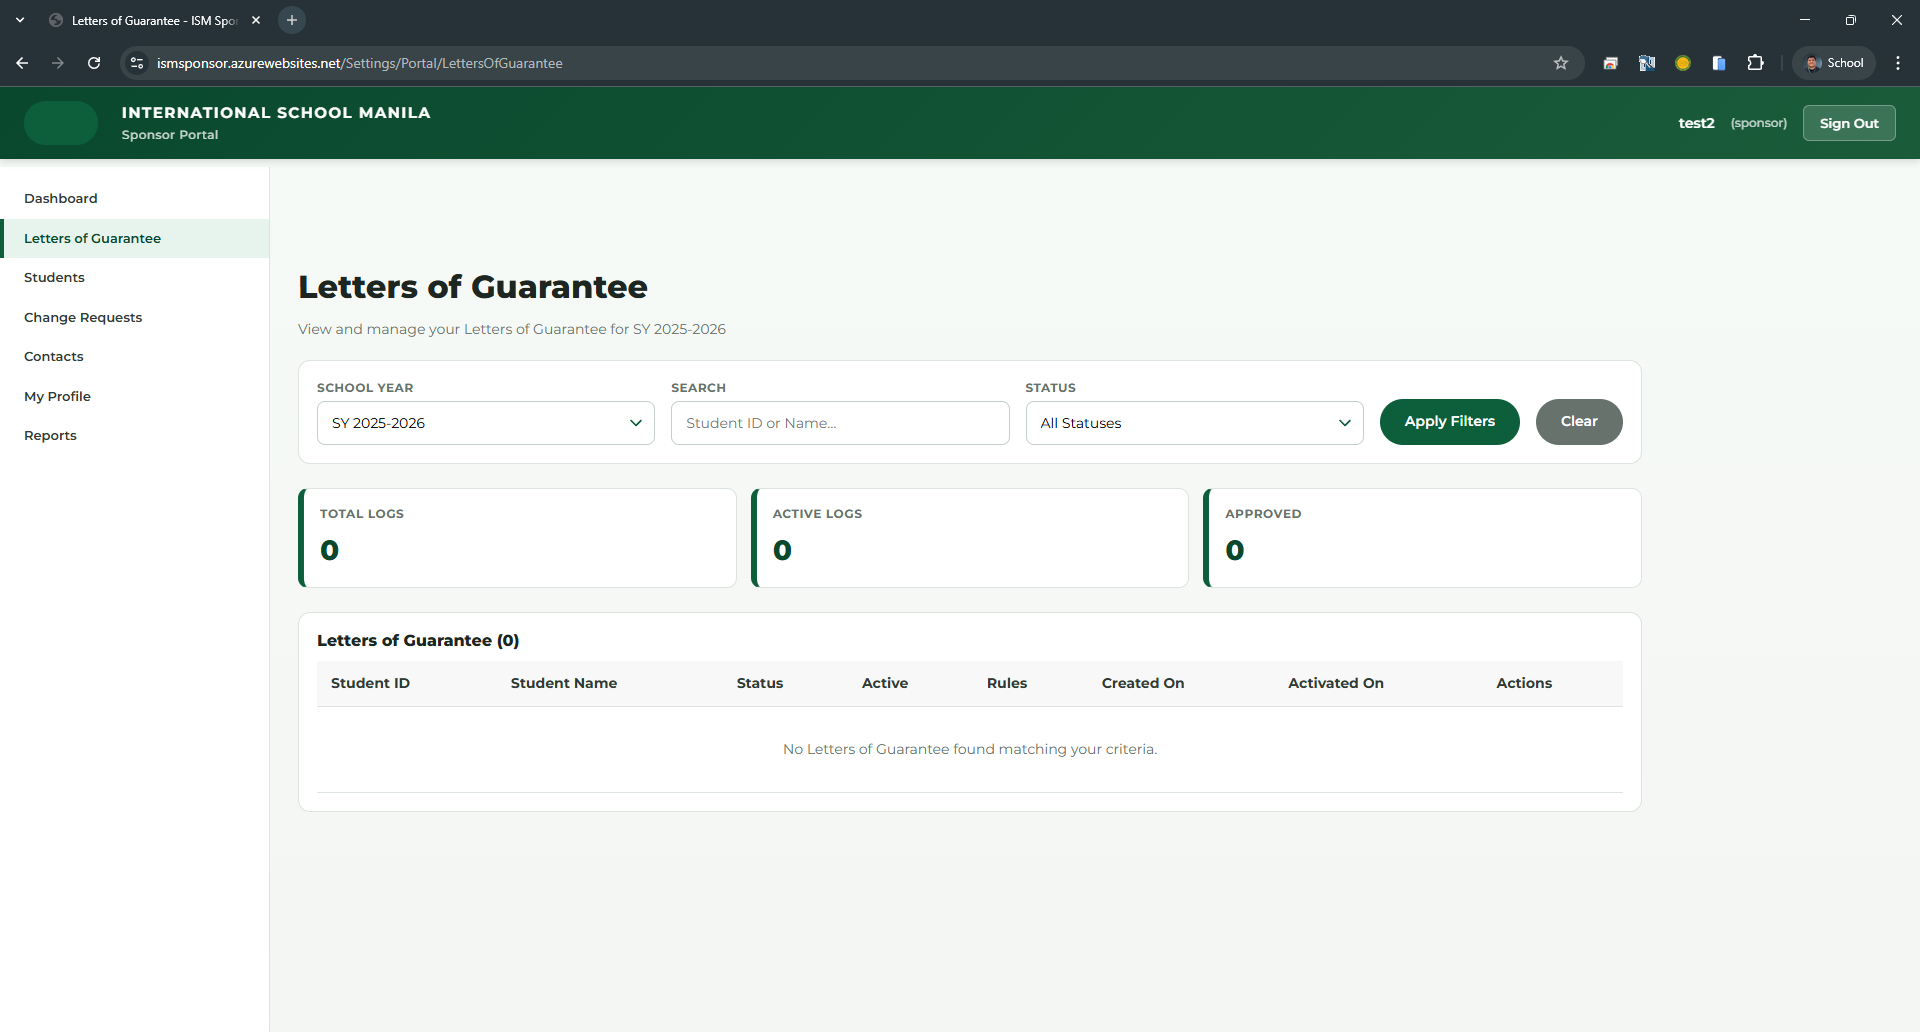
\includegraphics[width=0.90\linewidth]{images/current-interface/sponsor_logs.png}
        \caption{Sponsor-facing Letters of Guarantee page}
        \label{fig:current-sponsor-logs}
    \end{figure}

    \noindent Figure~\ref{fig:current-sponsor-logs} details the sponsor-facing LoG page, where sponsor users can review only the LoG records associated with their own organization. The figure is included to show how the pilot provides sponsor visibility without exposing internal administrative functions.

    \begin{figure}[H]
        \centering
        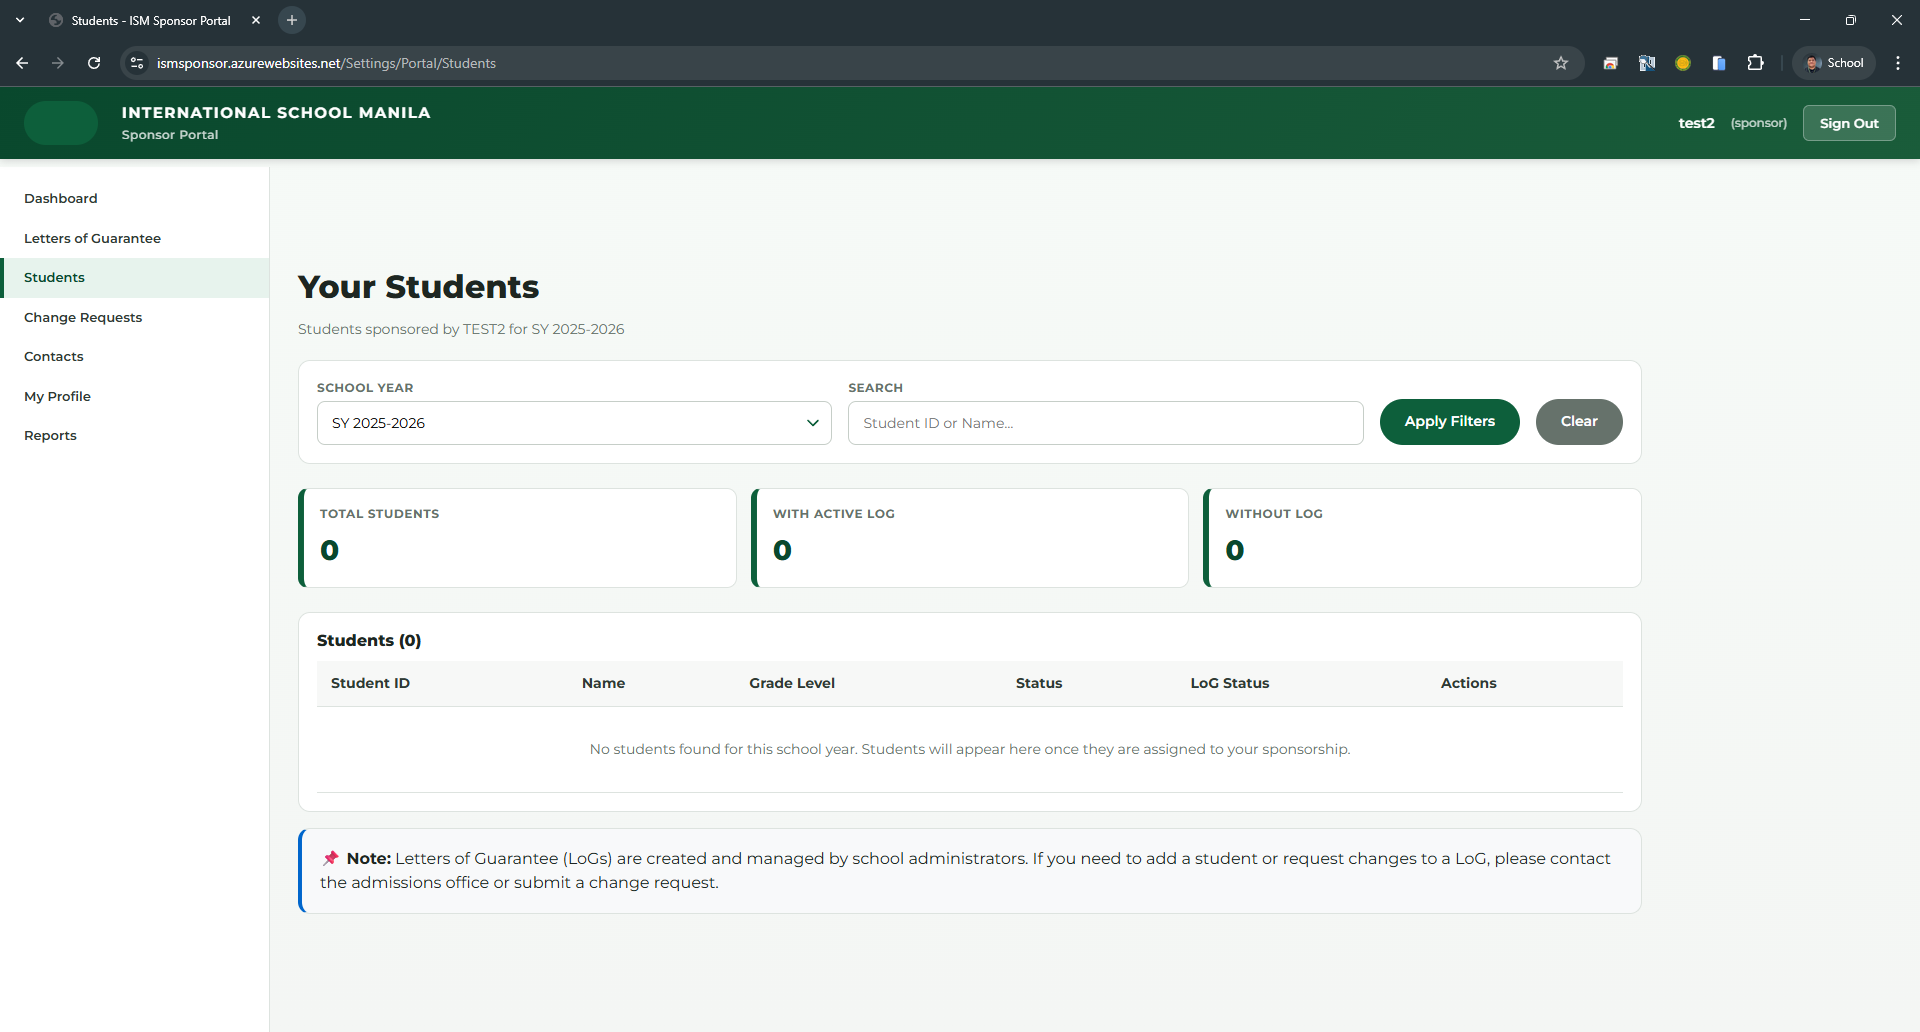
\includegraphics[width=0.90\linewidth]{images/current-interface/sponsor_students.png}
        \caption{Sponsor-facing Students page showing assigned students}
        \label{fig:current-sponsor-students}
    \end{figure}

    \noindent Figure~\ref{fig:current-sponsor-students} details the sponsor-facing Students page, where sponsor users can view students linked to their sponsor account within the permitted scope. The figure is included to show how sponsor-student relationships are presented as controlled records rather than informal references.
    \clearpage

    \subsubsection{Change Requests and Sponsor Self-Service}
    
    The deployed pilot comes with sponsor self-service option to submit and review change requests. These screens minimize the informal handling of update and help manage the governance process that sponsor profile updates are to be reviewed prior to making changes to sponsor master.

    \begin{figure}[H]
        \centering
        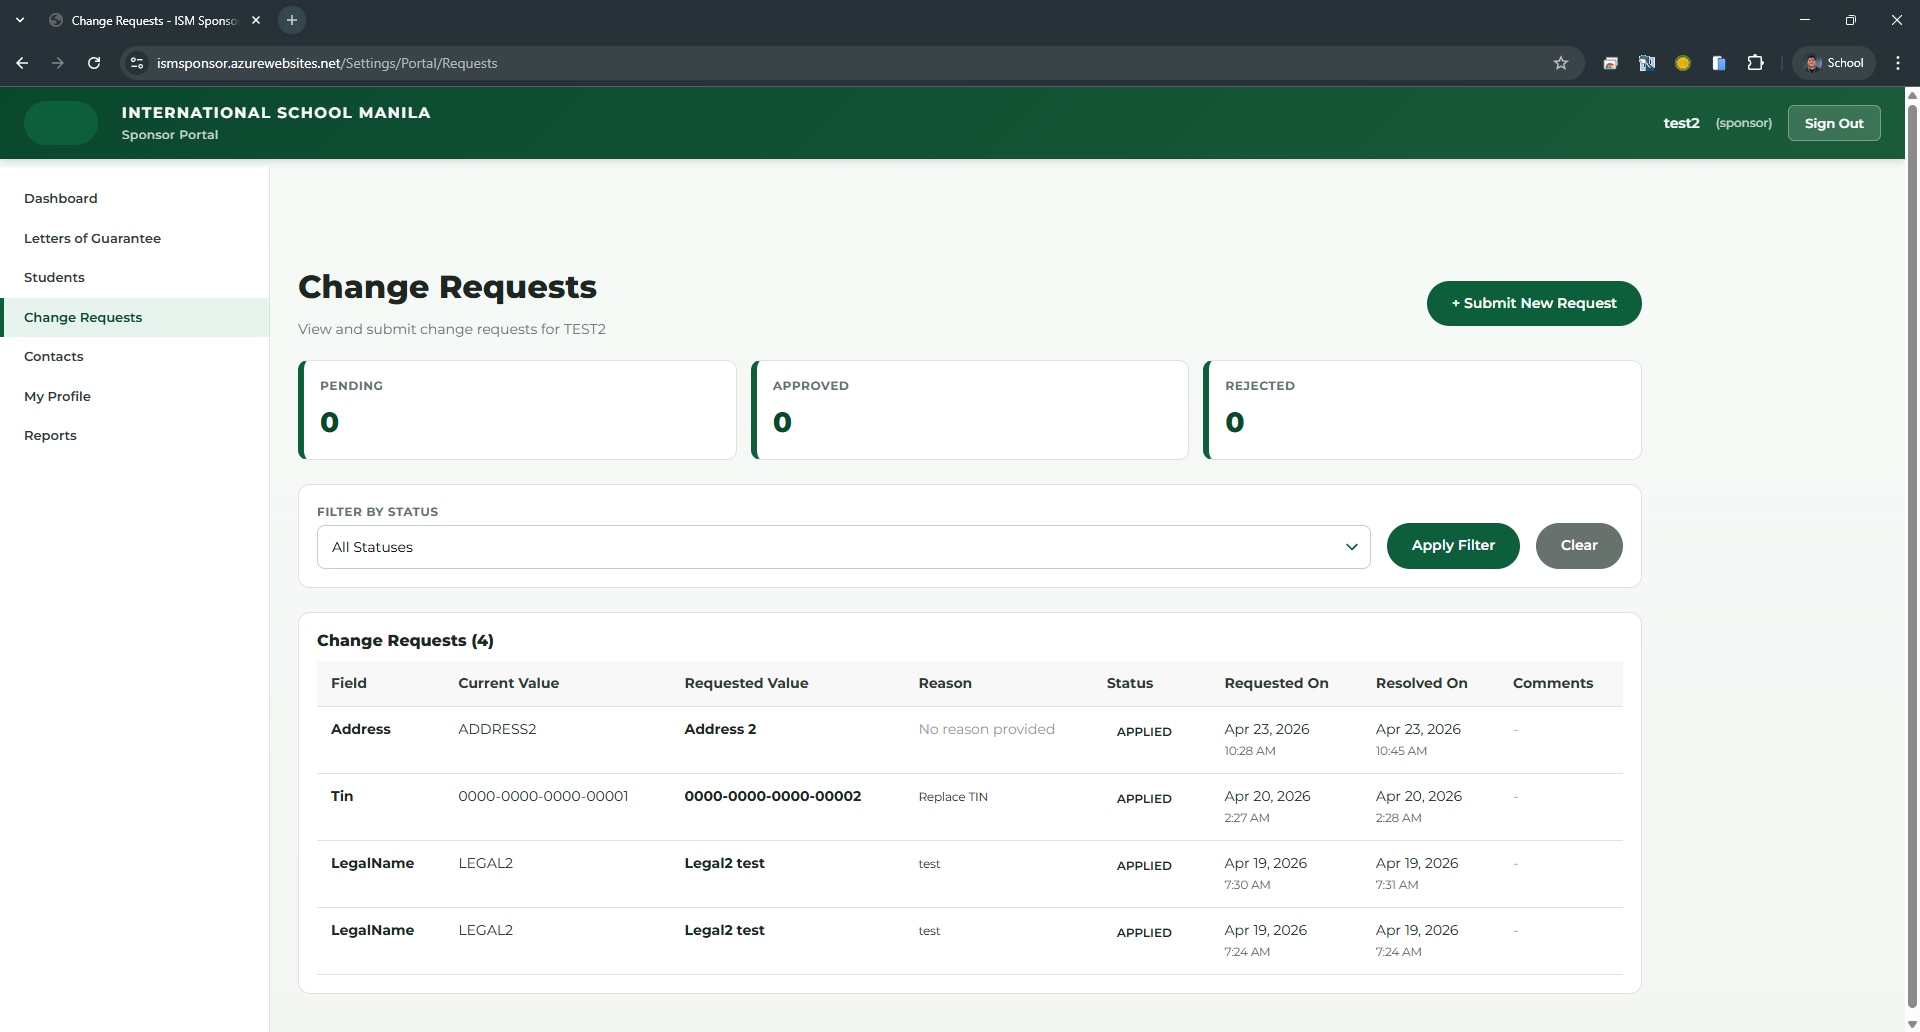
\includegraphics[width=0.90\linewidth]{images/current-interface/sponsor_change_requests.png}
        \caption{Sponsor change requests page in the sponsor-facing portal}
        \label{fig:current-sponsor-change-requests}
    \end{figure}

    \noindent Figure~\ref{fig:current-sponsor-change-requests} details the sponsor change-request page, where sponsors can submit and monitor requested updates to controlled profile information. The figure is included to show how the portal supports sponsor self-service while preserving staff review before changes affect the Sponsor Master.

    \begin{figure}[H]
        \centering
        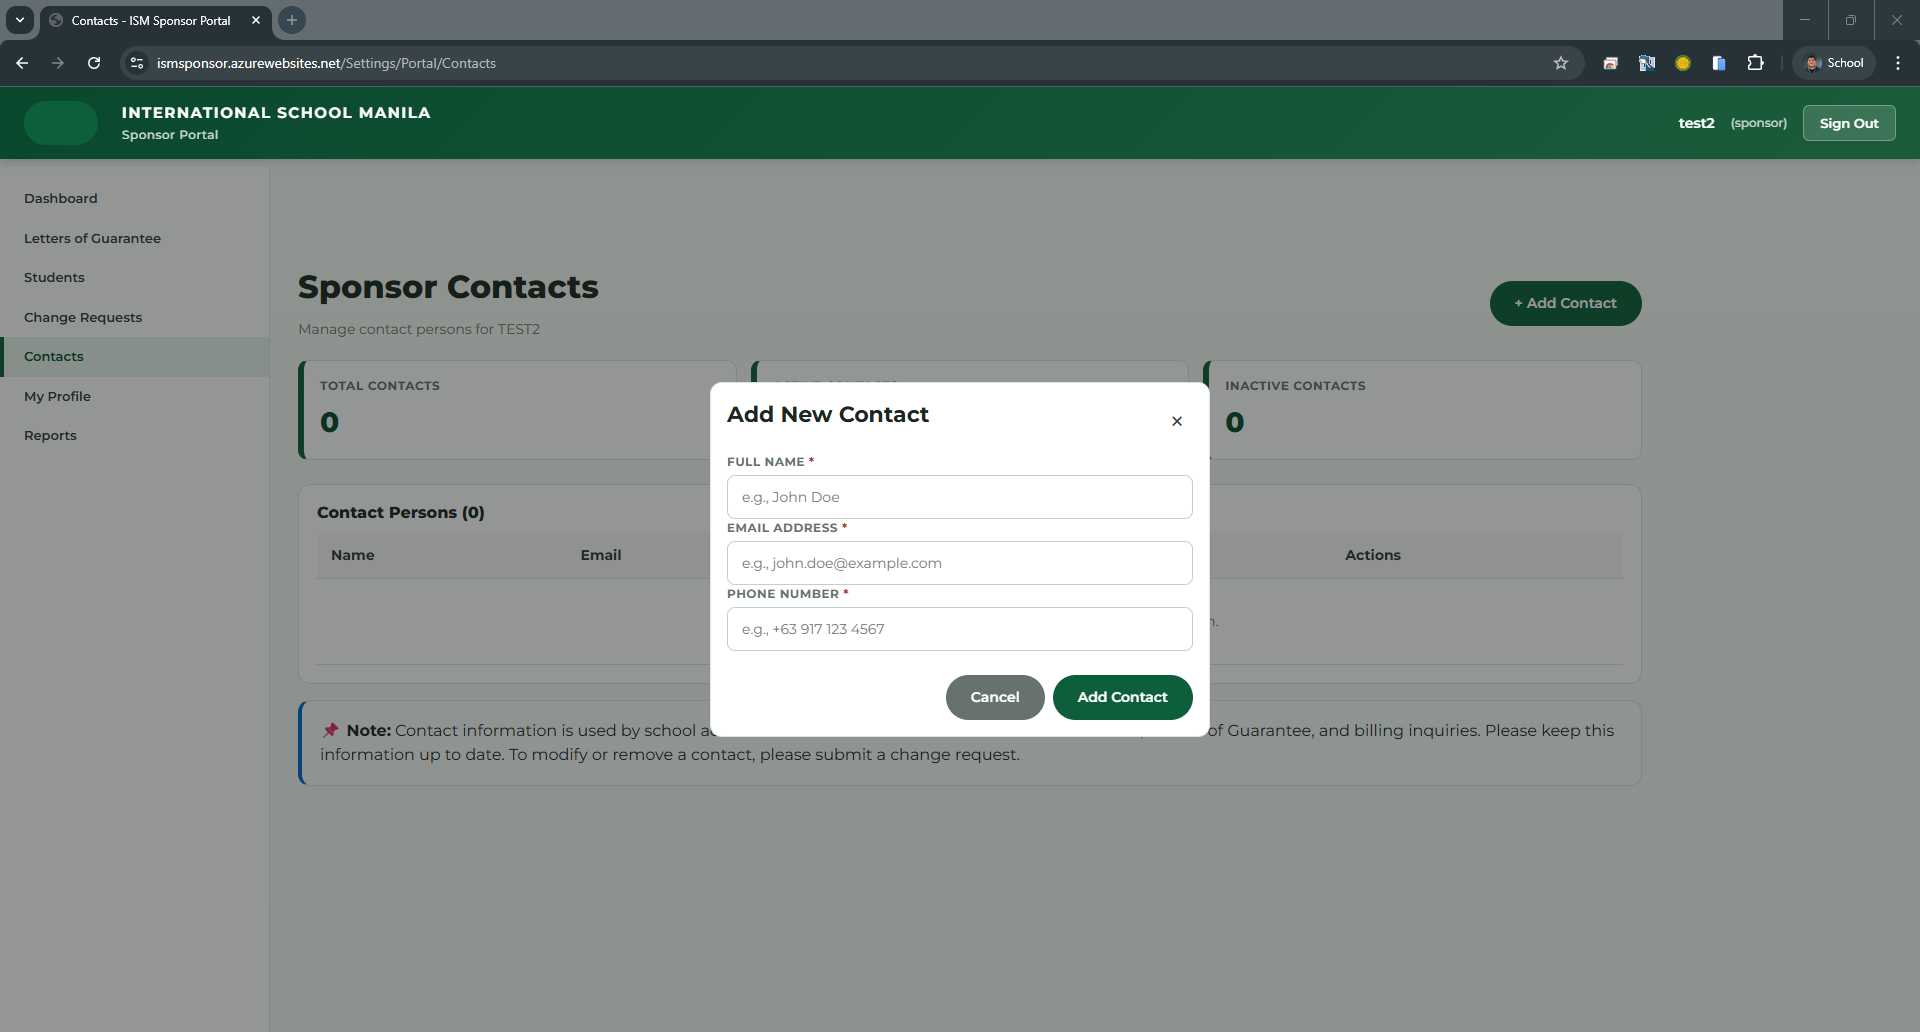
\includegraphics[width=0.90\linewidth]{images/current-interface/sponsor_add_contact.png}
        \caption{Add New Contact page for sponsor self-service updates}
        \label{fig:current-sponsor-add-contact}
    \end{figure}

    \noindent Figure~\ref{fig:current-sponsor-add-contact} details the sponsor self-service contact form, which allows a sponsor to request or add contact information through a controlled workflow. The figure is included to show how contact updates can be captured in structured form instead of being handled only through email or manual follow-up.
    \clearpage
    % FORMAT HIGHLIGHT: subsubsection heading
    % FORMAT HIGHLIGHT: LaTeX-safe conversion only; source wording retained
    
    \subsubsection{Reports and Monitoring Views}
    
    There is a role-aware Reports page in the deployed pilot. Administrative users will have access to administrative and monitoring reports, and Sponsor users will have access to reports for their own LoG and their students. This separation of report based on role helps the operational review without revealing information outside the boundary of each user's permission.
    
    \setlength{\LTleft}{0pt}
    \setlength{\LTright}{\fill}
    \begin{longtable}{>{\raggedright\arraybackslash}p{0.20\linewidth}
            >{\raggedright\arraybackslash}p{0.72\linewidth}}
    \caption{Implemented report access by role}\label{table:implemented-report-access}\\
    \toprule
    \textbf{Role} & \textbf{Reports available in the deployed pilot} \\
    \midrule
    \endfirsthead
    \caption[]{Implemented report access by role (continued)}\\
    \toprule
    \textbf{Role} & \textbf{Reports available in the deployed pilot} \\
    \midrule
    \endhead
    \midrule
    \multicolumn{2}{r}{\textit{Continued on next page}}\\
    \endfoot
    \bottomrule
    \endlastfoot
    \textbf{Administrator} & LoG Activity; Coverage Decisions; Sponsor Master; Sync Status; Audit Activity; Coverage Rules; Reconciliation Report; Coverage Tracking. \\
            \textbf{Admissions} & Coverage Tracking. \\
            \textbf{Cashier} & Reconciliation Report. \\
            \textbf{Sponsor} & My Letters of Guarantee; My Students. \\
    \end{longtable}

    Table~\ref{table:implemented-report-access} is placed before the report screenshots so the reader can first see the report permissions, then visually confirm how report access appears in the interface. Figure~\ref{fig:current-admin-reports} documents the staff-facing administrative reports page, while Figure~\ref{fig:current-sponsor-reports} documents the sponsor-facing reports page limited to sponsor-specific outputs.

    \begin{figure}[H]
        \centering
        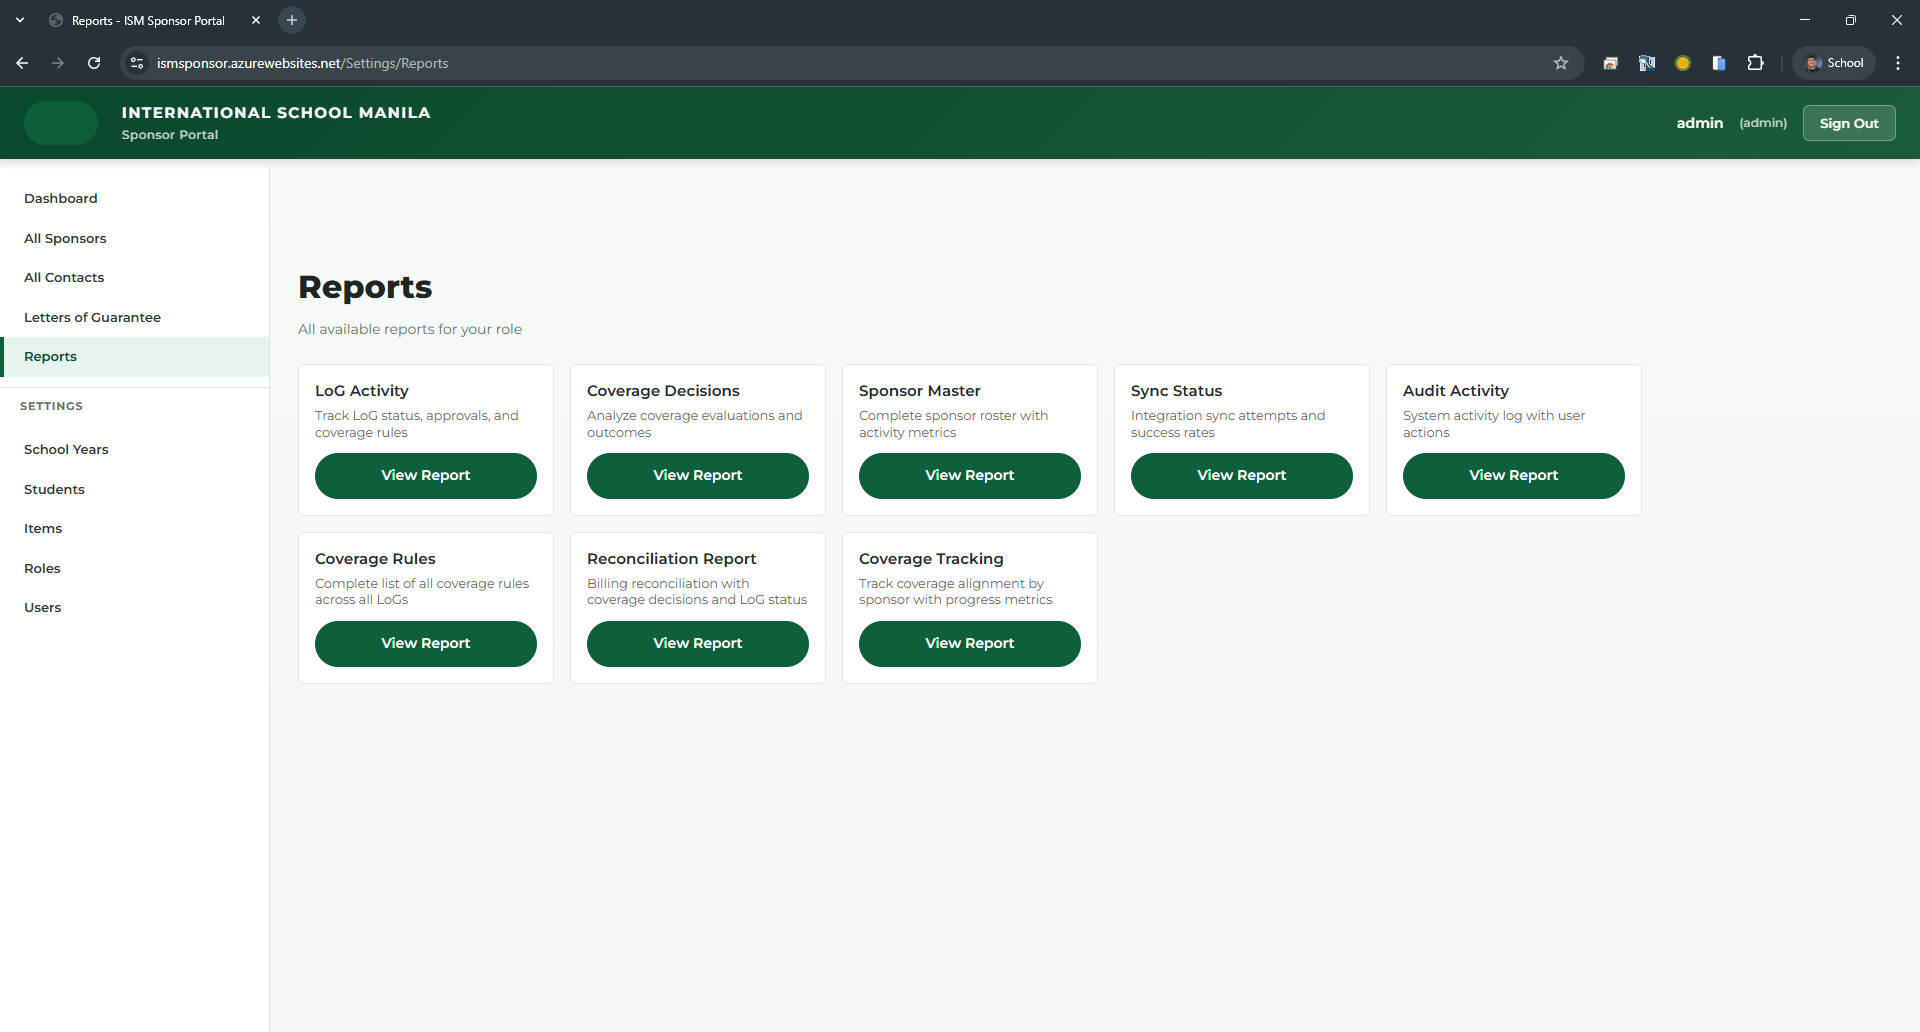
\includegraphics[width=0.90\linewidth]{images/current-interface/admin_reports.png}
        \caption{Administrator reports page in the current deployed pilot web application}
        \label{fig:current-admin-reports}
    \end{figure}

    \noindent Figure~\ref{fig:current-admin-reports} details the Administrator reports page, where staff can access administrative, audit, coverage, reconciliation, and monitoring-related reports. The figure is included to show how the pilot supports internal review of sponsor records, coverage decisions, and operational activity.

    \begin{figure}[H]
        \centering
        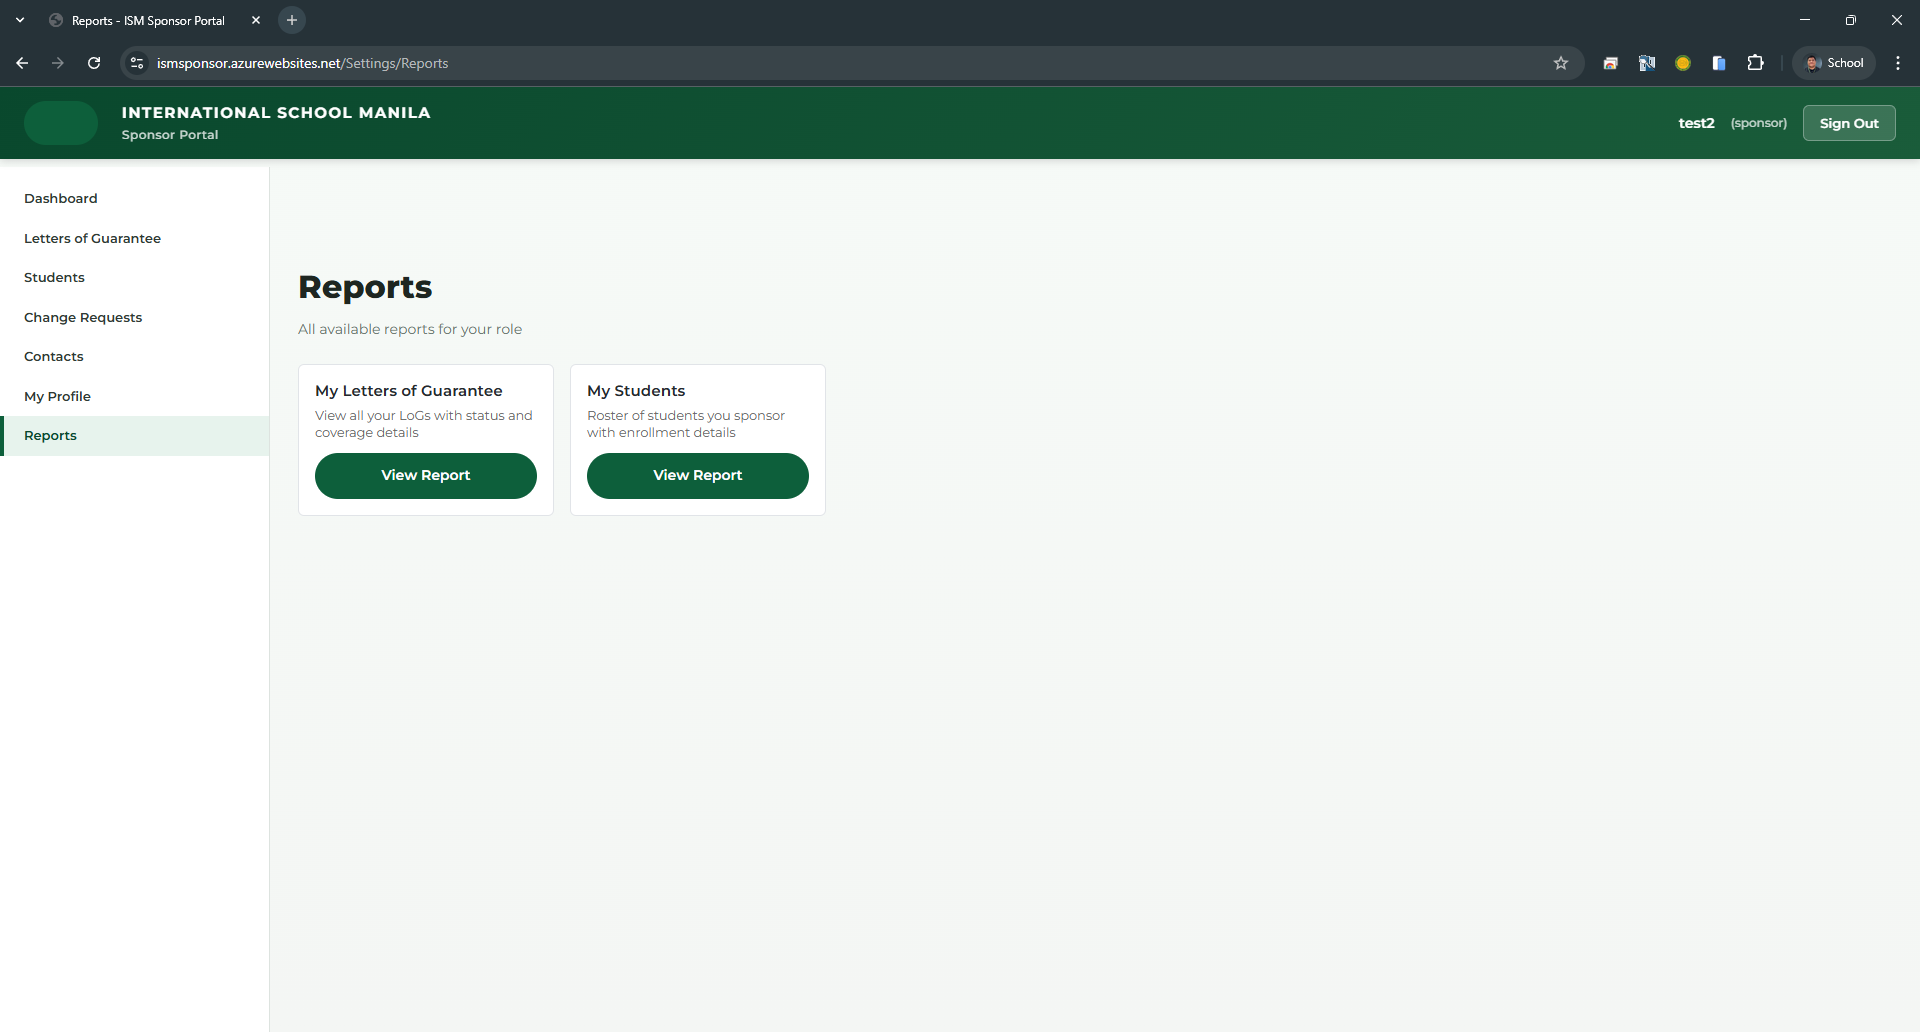
\includegraphics[width=0.90\linewidth]{images/current-interface/sponsor_reports.png}
        \caption{Sponsor reports page in the sponsor-facing portal}
        \label{fig:current-sponsor-reports}
    \end{figure}

    \noindent Figure~\ref{fig:current-sponsor-reports} details the sponsor-facing reports page, where report access is limited to sponsor-specific LoG and student outputs. The figure is included to show how reporting is separated by role so that external sponsors can review their own records without accessing institutional or other sponsor data.

    \subsubsection{Administrative Settings and Data Maintenance}
    
    Administrative settings are taken care of through unique pages for School Years, Students, Items, Roles, and Users. These pages store the reference data required for the pilot system to work. The records for school years create active periods, student records provide data for sponsors and status, item records provide data for coverage, role records control access, and user records provide data for user accounts.    

    \begin{figure}[H]
        \centering
        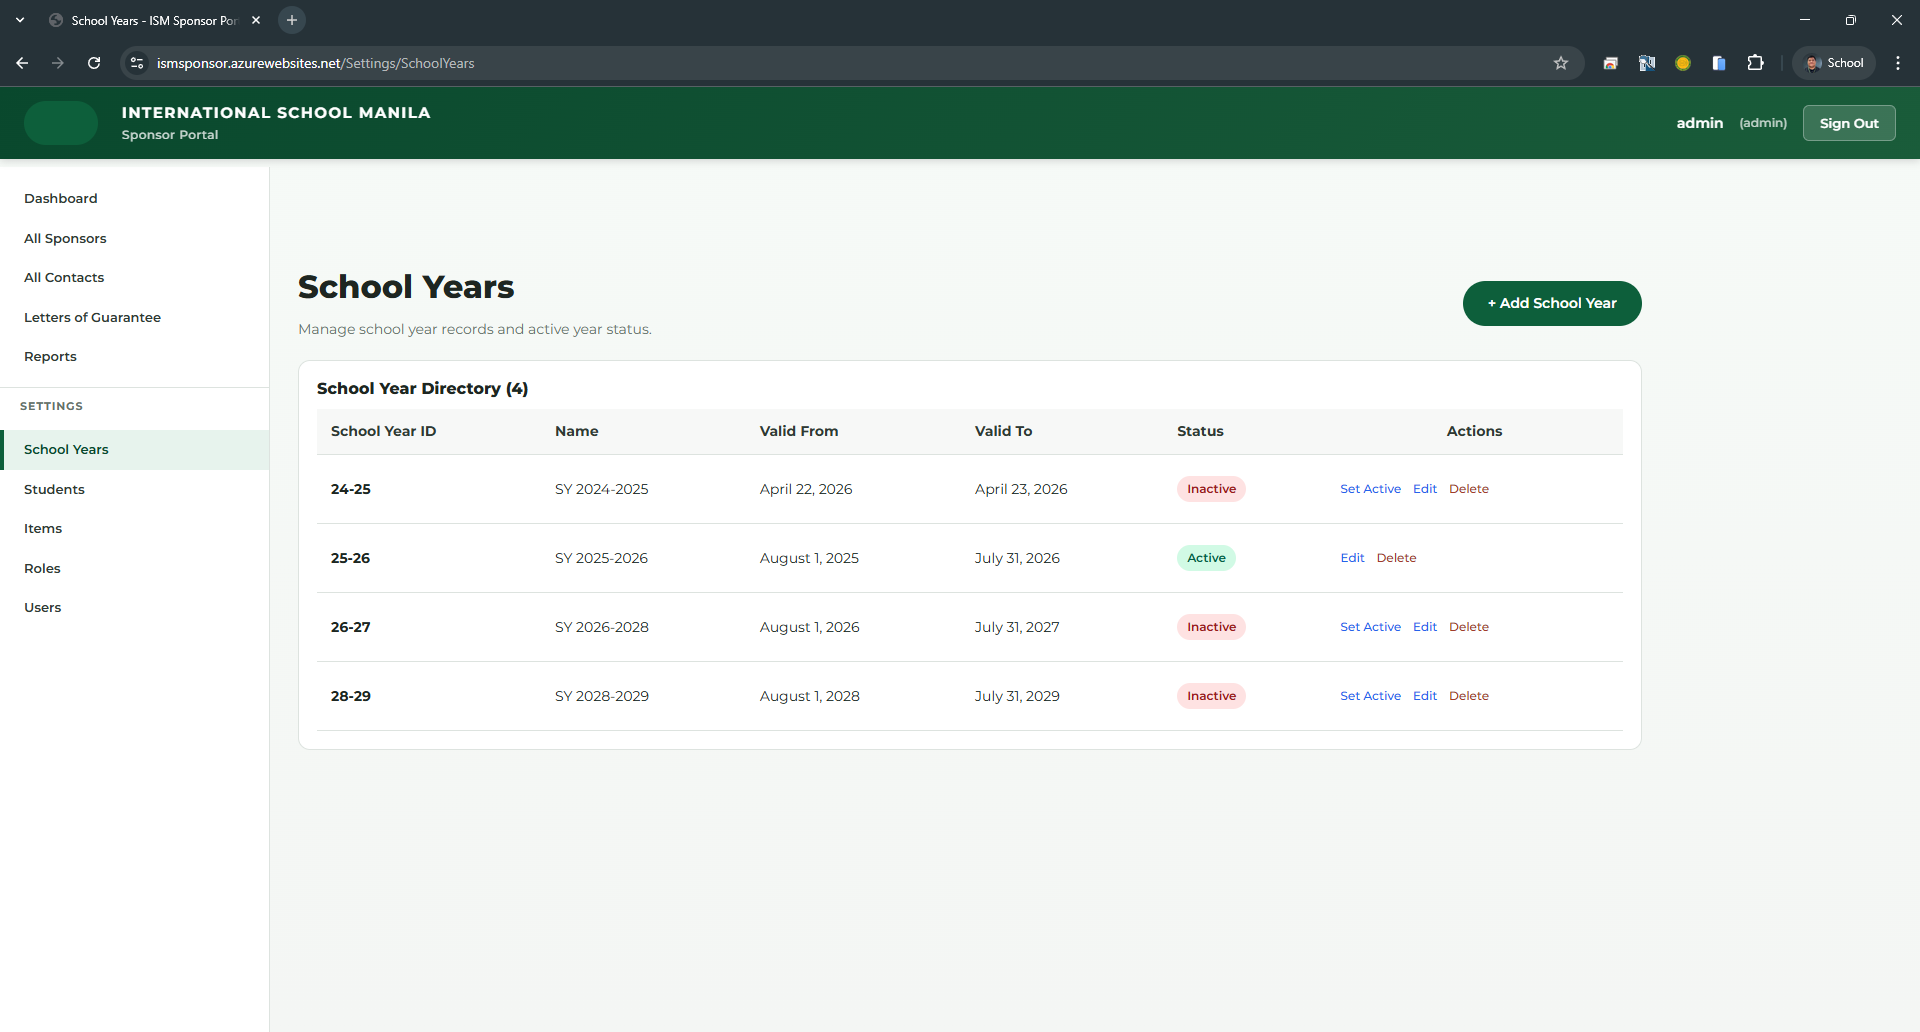
\includegraphics[width=0.90\linewidth]{images/current-interface/admin_school_years.png}
        \caption{School Years management page}
        \label{fig:current-school-years}
    \end{figure}

    \noindent Figure~\ref{fig:current-school-years} details the School Years management page, which maintains active periods used by dashboard, LoG, coverage, and reporting views. The figure is included to show how date-based coverage and reporting depend on controlled school-year reference data.

    \begin{figure}[H]
        \centering
        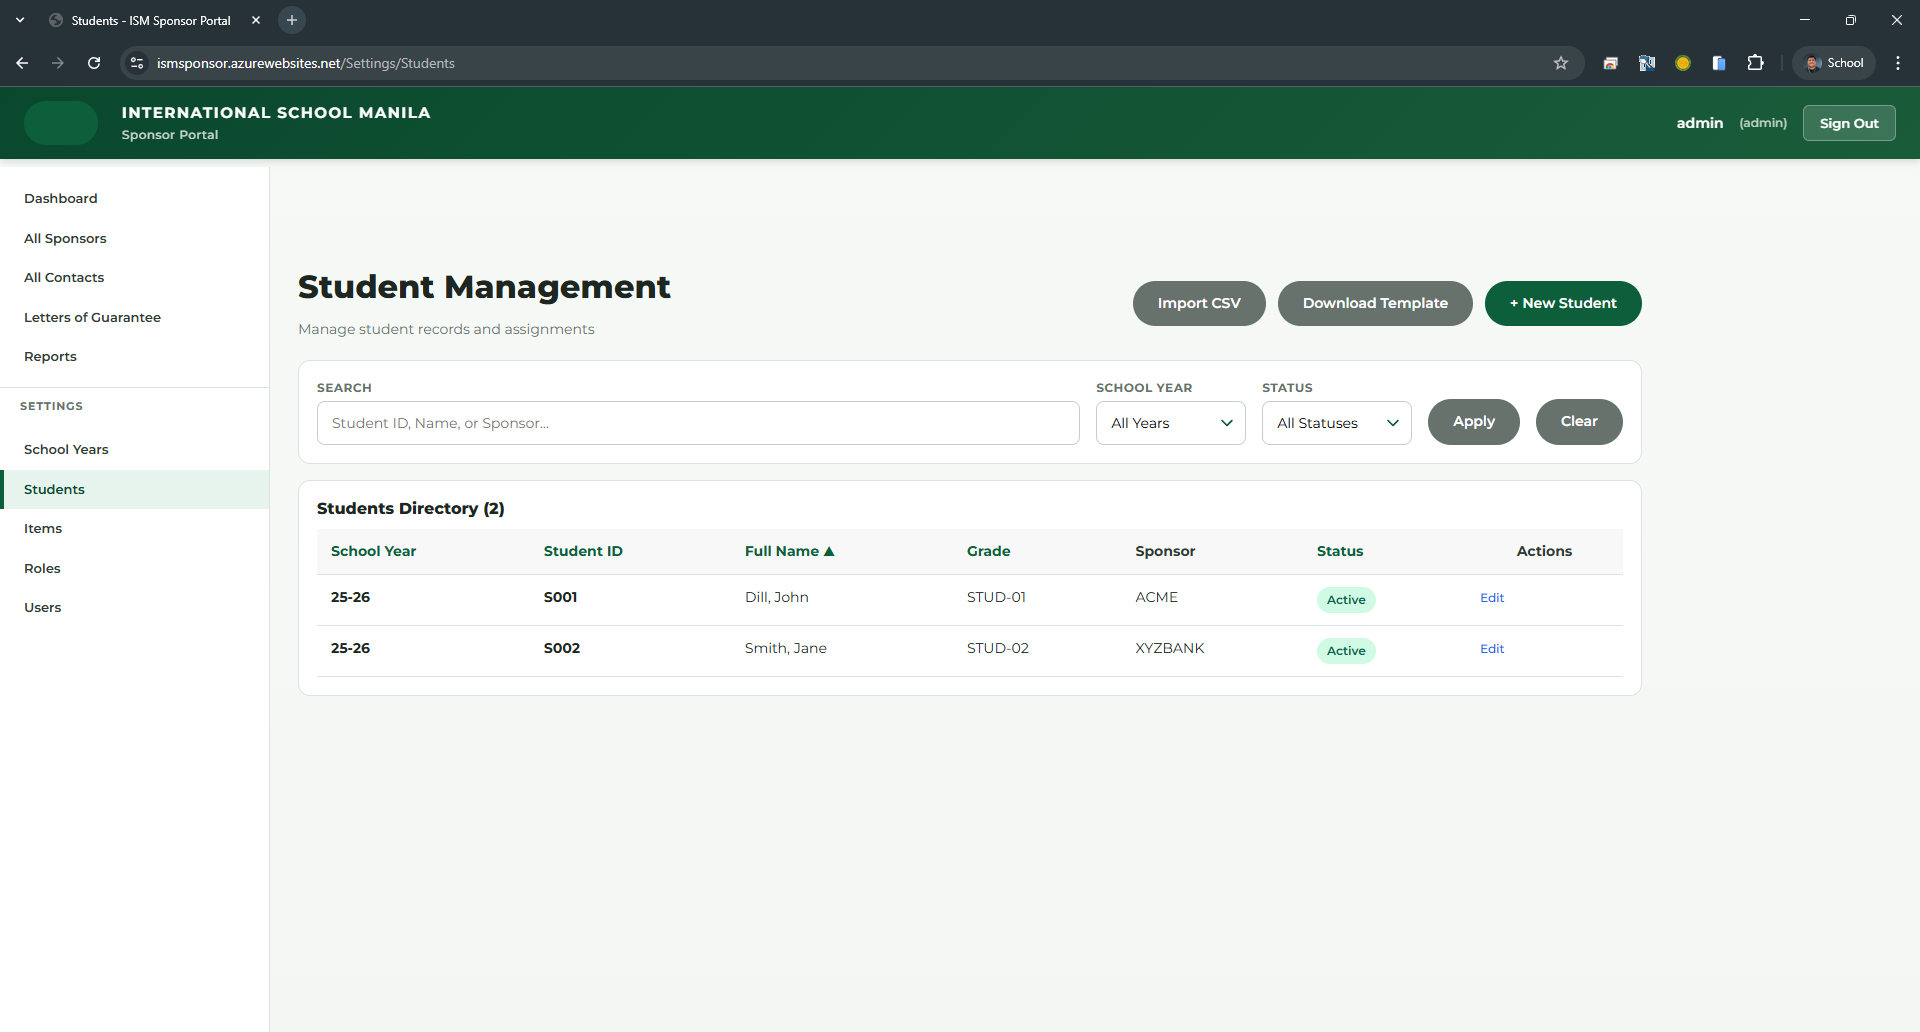
\includegraphics[width=0.90\linewidth]{images/current-interface/admin_students.png}
        \caption{Student Management page}
        \label{fig:current-student-management}
    \end{figure}

    \noindent Figure~\ref{fig:current-student-management} details the Student Management page, where student records can be searched and reviewed by school year, sponsor, and status. The figure is included to show how student references support sponsor assignment and LoG coverage validation.

    \begin{figure}[H]
        \centering
        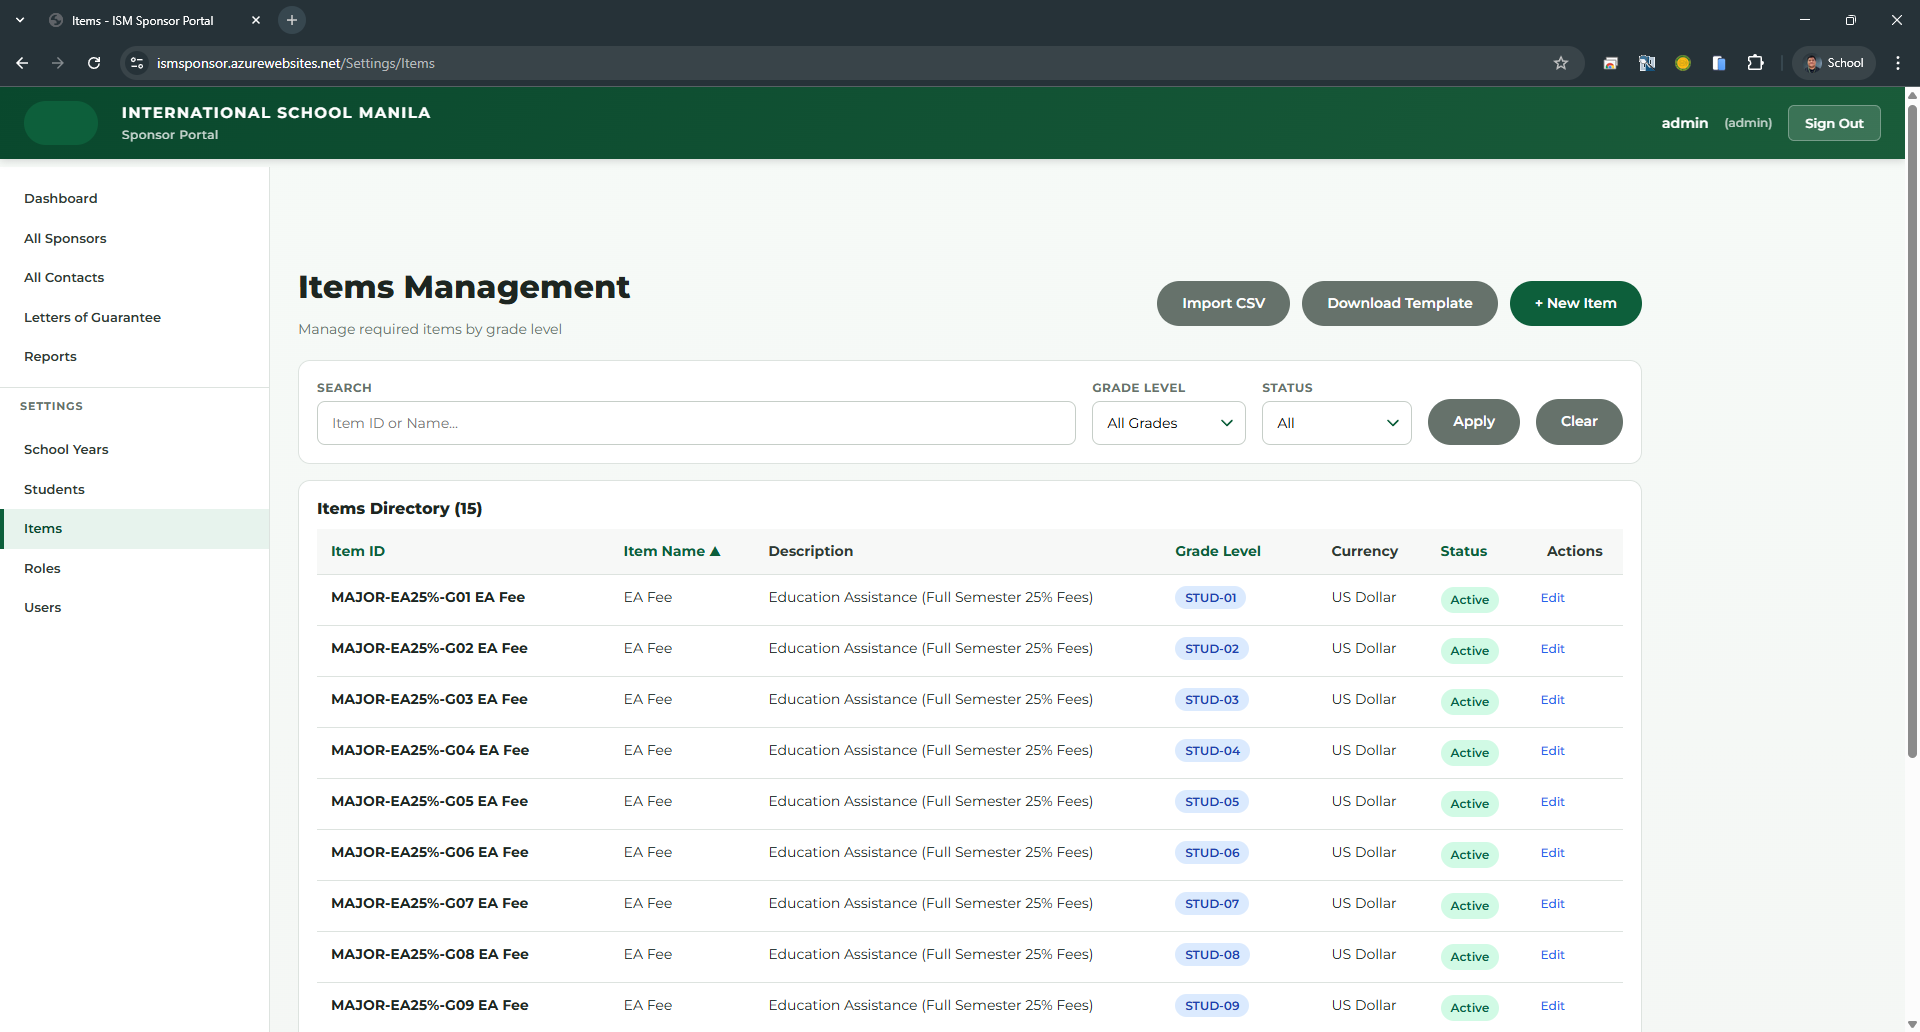
\includegraphics[width=0.90\linewidth]{images/current-interface/admin_items.png}
        \caption{Items Management page}
        \label{fig:current-items-management}
    \end{figure}

    \noindent Figure~\ref{fig:current-items-management} details the Items Management page, which maintains the charge items used in coverage evaluation. The figure is included to show how item-level reference data supports deterministic matching between a charge and the related LoG coverage rule.

    \begin{figure}[H]
        \centering
        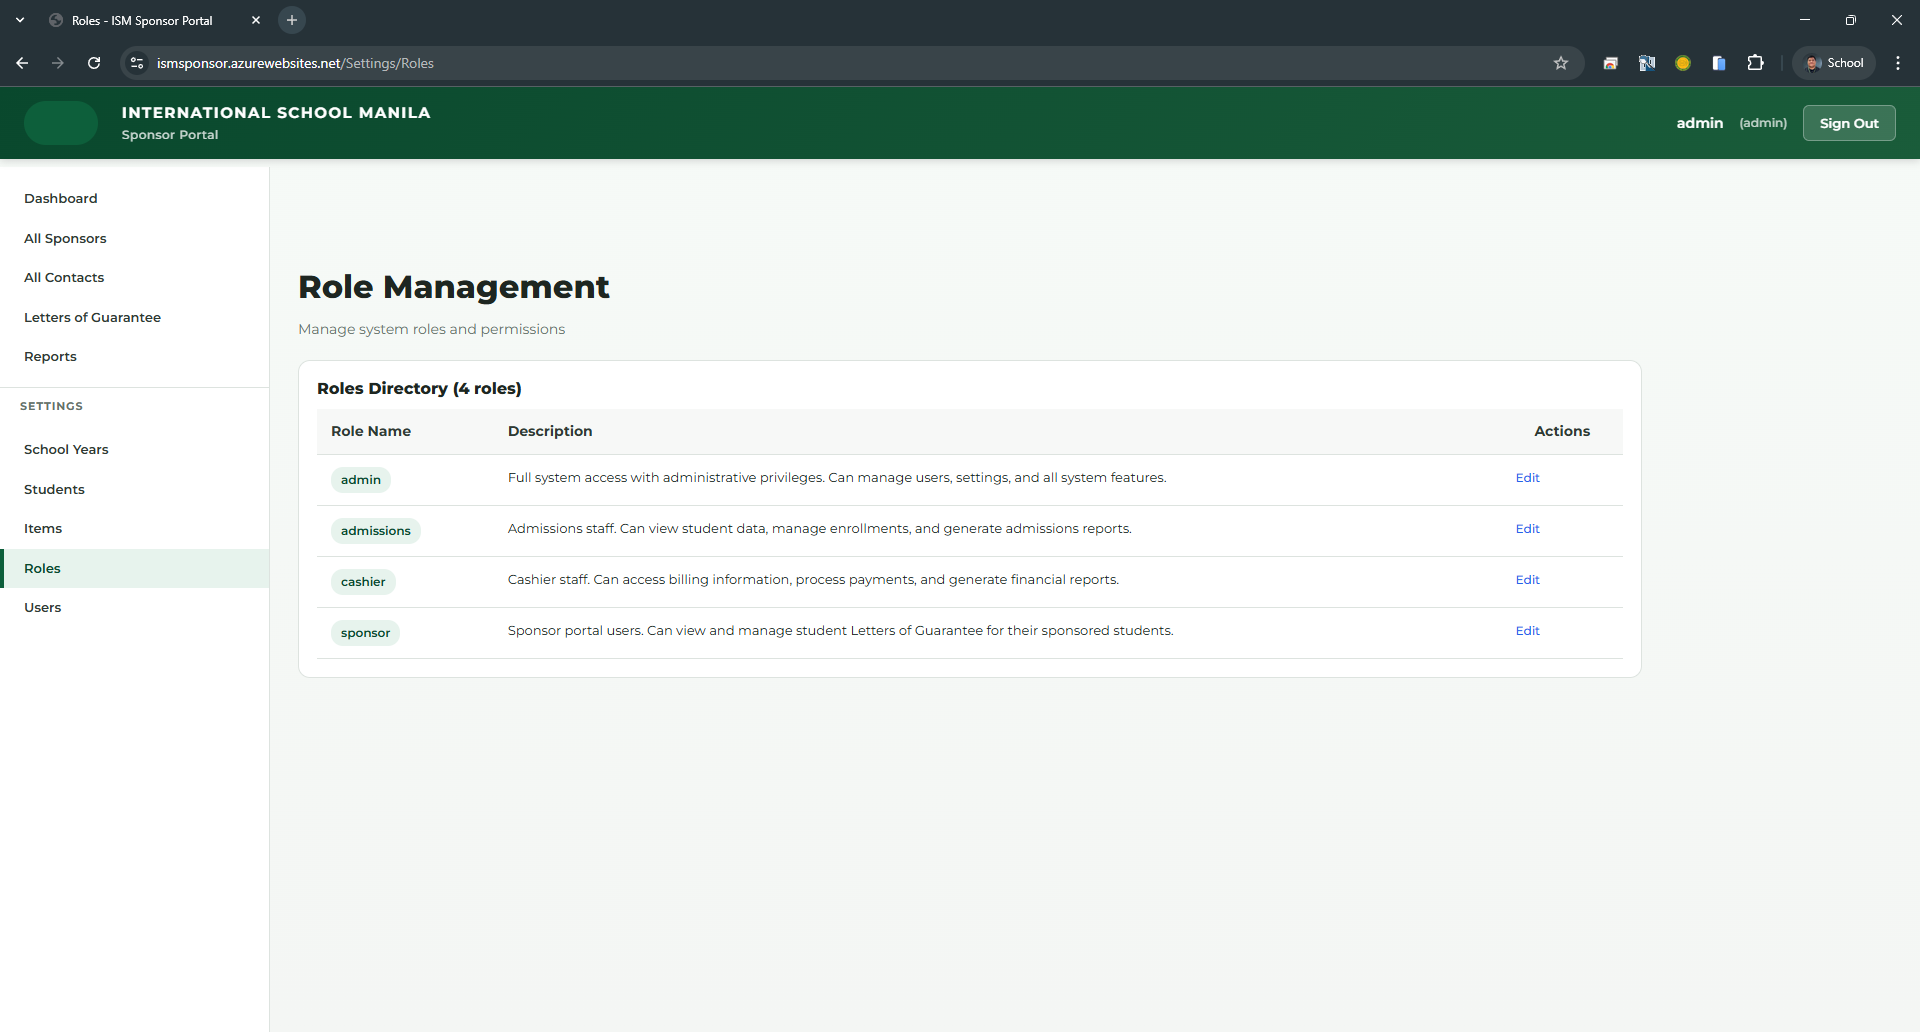
\includegraphics[width=0.90\linewidth]{images/current-interface/admin_roles.png}
        \caption{Role Management page}
        \label{fig:current-role-management}
    \end{figure}

    \noindent Figure~\ref{fig:current-role-management} details the Role Management page, which defines role records used for access control. The figure is included to show how the pilot separates administrative, admissions, cashier, and sponsor permissions.

    \begin{figure}[H]
        \centering
        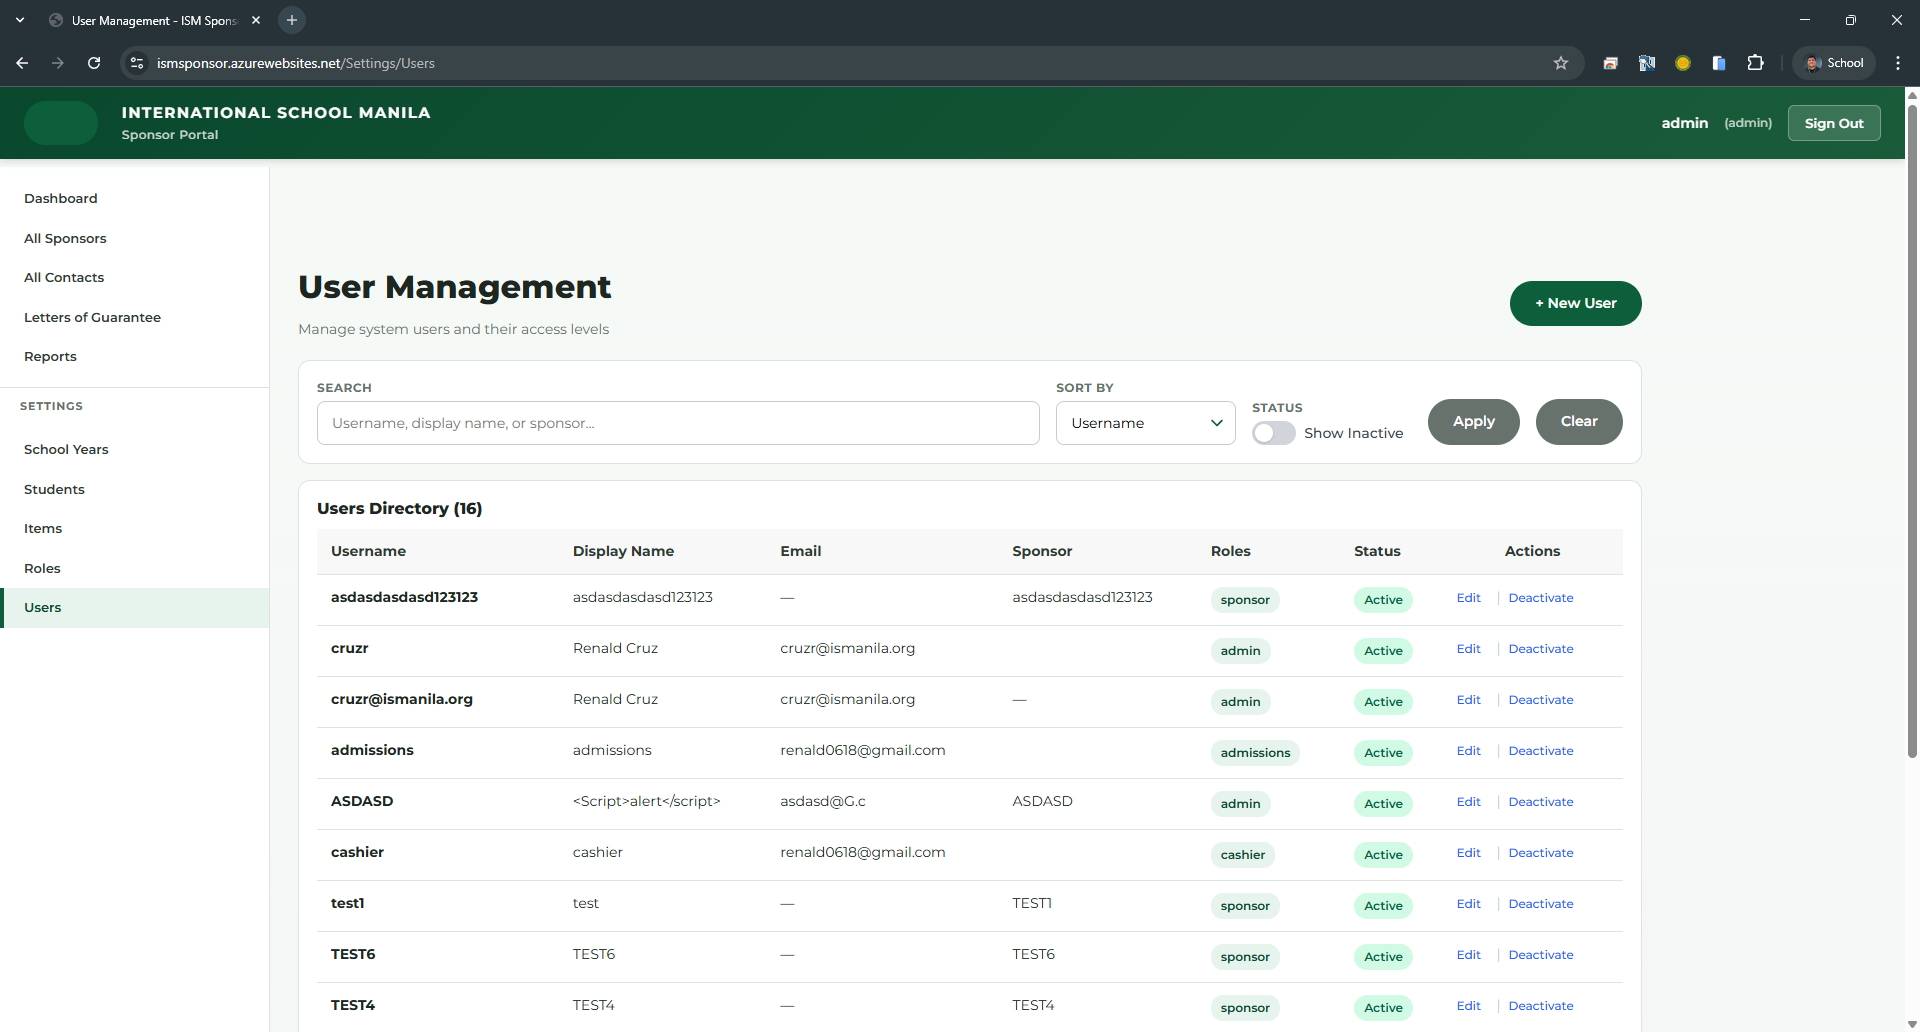
\includegraphics[width=0.90\linewidth]{images/current-interface/admin_users.png}
        \caption{User Management page}
        \label{fig:current-user-management}
    \end{figure}

    \noindent Figure~\ref{fig:current-user-management} details the User Management page, where user accounts, role assignments, and sponsor account links are administered. The figure is included to show how access governance is maintained for both internal users and sponsor-facing accounts.
    \clearpage


            %PROJECT ASSESSMENT
            % Put the project assessment here

\section{PROJECT ASSESSMENT}

This chapter provides the assessment basis for the finished pilot web app for the Sponsor Management and Letter of Guarantee Coverage Integration System. This assessment was meant to see if the system that has been implemented is working, access control, testing evidence, and non-functional checks are adequate to show a capstone demonstration for the International School Manila environment for controlled pilot review.

The Project Assessment chapter provides a description of how the system was assessed. The results of the tests in detail are given in the Results and Discussion chapter. This separation lets the assessment method be evident while keeping the results chapter to justify the final assessment based on the actual Passed and Failed results from testing.

The assessment used a binary result basis. A test item was marked as \textbf{Passed} when the tested function, workflow, control, or system response produced the expected result. A test item was marked as \textbf{Failed} when the expected result was not achieved, the workflow could not be completed, or the system behavior required correction before it could support the intended pilot use.

\setlength{\LTleft}{0pt}
\setlength{\LTright}{\fill}
\begin{longtable}{>{\raggedright\arraybackslash}p{0.22\linewidth}
>{\raggedright\arraybackslash}p{0.30\linewidth}
>{\raggedright\arraybackslash}p{0.24\linewidth}
>{\raggedright\arraybackslash}p{0.18\linewidth}}
\caption{Assessment basis and result alignment}\label{table:assessment-basis}\\
\toprule
\textbf{Assessment area} & \textbf{Basis of assessment} & \textbf{Evidence source} & \textbf{Result location} \\
\midrule
\endfirsthead
\caption[]{Assessment basis and result alignment (continued)}\\
\toprule
\textbf{Assessment area} & \textbf{Basis of assessment} & \textbf{Evidence source} & \textbf{Result location} \\
\midrule
\endhead
\midrule
\multicolumn{4}{r}{\textit{Continued on next page}}\\
\endfoot
\bottomrule
\endlastfoot
Consolidated appendix register & All supporting PDF evidence was organized into a single appendix map before presenting the detailed test-result tables. & Appendix evidence register covering the UAT, final comparison, security, performance, and Swagger/OpenAPI supporting PDFs. & Appendix A.1. \\
Functional and API testing & Sponsor, LoG, coverage, reporting, audit, test-account, and endpoint behavior were checked against expected pilot functions. & Final automated and manual test comparison report. & Results and Discussion; Appendix A.3. \\
User acceptance testing & Administrator, Admissions, Cashier, and Sponsor workflows were assessed using role-based tasks and a Passed or Failed result basis. & UAT response summary and role-based workflow evidence. & Results and Discussion; Appendix A.2. \\
Security testing & Authentication, authorization, session handling, CSRF protection, SQL injection prevention, audit logging, security headers, and OWASP-aligned controls were reviewed. & Internal security checklist, ZAP comparison, and security fixes report. & Results and Discussion; Appendix A.4. \\
Performance testing & Load and response-time behavior were checked using Postman test evidence for the 5,000 and 10,000 virtual-user scenarios. & Postman load-test evidence and performance reports. & Results and Discussion; Appendix A.5. \\
Deployment readiness & Accessibility, Swagger availability, known issues, and endpoint-consumption readiness were reviewed for controlled pilot use. & Deployment checks, Swagger/OpenAPI summary, and known-issue evidence. & Results and Discussion; Appendix A.6. \\
\end{longtable}

Table~\ref{table:assessment-basis} shows the test areas, evidence sources, and result locations used to assess the pilot. A consolidated map of the appendix evidence is provided in Appendix~A.1 before the detailed appendix result tables. The tables in this chapter define the assessment basis only. The actual Passed and Failed results are discussed in the Results and Discussion chapter.

\subsection{Functional and User Acceptance Testing}

Functional and user acceptance testing assessed whether the implemented workflows could be completed by the supported role groups. The assessment covered the four implemented roles: Administrator, Admissions, Cashier, and Sponsor. The role groups were used to define task coverage and access boundaries. They were not used as a separate measure of project significance.

\setlength{\LTleft}{0pt}
\setlength{\LTright}{\fill}
Table~\ref{table:user-testing-role-groups-task-coverage} identifies the user groups and task areas used to assess whether the pilot supported the expected role-based workflows.

\begin{longtable}{>{\raggedright\arraybackslash}p{0.20\linewidth}
>{\raggedright\arraybackslash}p{0.72\linewidth}}
\caption{User-testing role groups and tested task coverage}\label{table:user-testing-role-groups-task-coverage}\\
\toprule
\textbf{Role group} & \textbf{Representative tested tasks} \\
\midrule
\endfirsthead
\caption[]{User-testing role groups and tested task coverage (continued)}\\
\toprule
\textbf{Role group} & \textbf{Representative tested tasks} \\
\midrule
\endhead
\midrule
\multicolumn{2}{r}{\textit{Continued on next page}}\\
\endfoot
\bottomrule
\endlastfoot
Administrator & Verified staff login, dashboard access, sponsor maintenance, sponsor-contact review, LoG activation controls, settings maintenance, user and role management, reports, exports, monitoring views, and audit-related outputs. \\
Admissions & Verified staff login, sponsor search, sponsor record review, sponsor-related updates where allowed, LoG viewing, student-related LoG records, workflow-status review, and restriction from administrative functions. \\
Cashier & Verified staff login, sponsor lookup, LoG review, coverage viewing, attachment review where permitted, report or reconciliation-related outputs, read-oriented access, and restriction from administrative actions. \\
Sponsor & Verified sponsor login, sponsor profile viewing, sponsor contact viewing, sponsor profile change-request submission, LoG status review, sponsor-specific coverage views, and restriction from internal staff functions. \\
\end{longtable}

\subsubsection{Success Metrics}

The assessment used Passed and Failed as the result basis. The following rules were applied when interpreting the functional and user-testing outcomes:

\begin{itemize}
    \item \textbf{Passed:} The tested function, workflow, access-control rule, data action, report output, or system response produced the expected result.
    \item \textbf{Failed:} The tested function, workflow, access-control rule, data action, report output, or system response did not produce the expected result, could not be completed, or required correction.
    \item \textbf{Pilot-readiness basis:} The pilot was considered acceptable for controlled review when the required functional and non-functional test areas passed, and any item requiring further action was corrected or documented for future production hardening.
\end{itemize}

\setlength{\LTleft}{0pt}
\setlength{\LTright}{\fill}
\begin{longtable}{>{\raggedright\arraybackslash}p{0.08\linewidth}
>{\raggedright\arraybackslash}p{0.17\linewidth}
>{\raggedright\arraybackslash}p{0.31\linewidth}
>{\raggedright\arraybackslash}p{0.36\linewidth}}
\caption{User-testing scenarios and pass/fail assessment basis}\label{table:user-testing-scenarios-pass-fail}\\
\toprule
\textbf{ID} & \textbf{Actor} & \textbf{Test scenario} & \textbf{Pass/fail basis} \\
\midrule
\endfirsthead
\caption[]{User-testing scenarios and pass/fail assessment basis (continued)}\\
\toprule
\textbf{ID} & \textbf{Actor} & \textbf{Test scenario} & \textbf{Pass/fail basis} \\
\midrule
\endhead
\midrule
\multicolumn{4}{r}{\textit{Continued on next page}}\\
\endfoot
\bottomrule
\endlastfoot
UT01 & Any role & Login and baseline access validation. & Passed if valid users reached the correct role-based page and invalid access was denied. Failed if login, redirection, or denial behavior did not work as expected. \\
UT02 & Any role & Role-based access-control enforcement. & Passed if restricted pages and actions were hidden, blocked, or denied. Failed if a role accessed unauthorized functions. \\
UT03 & Administrator / Admissions & Sponsor record creation. & Passed if a sponsor record was saved, displayed, and searchable after creation. Failed if the record was not saved or could not be retrieved. \\
UT04 & Administrator / Admissions & Validation and error messaging. & Passed if missing or invalid fields were blocked with a clear message. Failed if invalid data was saved or no message appeared. \\
UT05 & Administrator / Admissions & Sponsor record update and persistence. & Passed if updated sponsor values remained visible after saving, searching, and retrieval. Failed if changes were lost or displayed incorrectly. \\
UT06 & Administrator & Sponsor contact and supporting record maintenance. & Passed if sponsor contacts and related records could be reviewed or updated as expected. Failed if records could not be accessed, saved, or displayed correctly. \\
UT07 & Sponsor & Sponsor profile review and change request. & Passed if the sponsor could view profile information and submit an allowed change request. Failed if the profile or request workflow did not work. \\
UT08 & Administrator & Sponsor change-request review. & Passed if the Administrator could review and act on a submitted sponsor request. Failed if the request could not be reviewed or tracked. \\
UT09 & Any role; Administrator for activation & LoG list, coverage view, and activation controls. & Passed if users could search LoG records, view coverage, and perform activation controls according to role. Failed if LoG access or activation behavior was incorrect. \\
UT10 & Administrator & Report, audit, and traceability review. & Passed if reports, exports, activity records, or audit-related outputs showed traceable system actions. Failed if expected records were missing or inaccurate. \\
\end{longtable}

Table~\ref{table:user-testing-scenarios-pass-fail} aligns the user-testing scenarios with the same Passed and Failed basis used in the results. This ensures that the assessment criteria match the actual result format used for the pilot evaluation.

\subsection{Non-Functional Testing}

Non-functional testing assessed whether the pilot satisfied baseline quality expectations for controlled review. The non-functional assessment covered security, performance, deployment readiness, mobile responsiveness, and integration readiness.

\subsubsection{Security Testing}

Security testing assessed the system's baseline protection for sponsor and LoG-related data. The testing focused on authentication, authorization, input handling, session behavior, request protection, security headers, audit logging, and security hardening. The evidence came from browser-based testing, role-based test accounts, an internal security checklist, ZAP by Checkmarx, and security-fix verification.

\setlength{\LTleft}{0pt}
\setlength{\LTright}{\fill}
Table~\ref{table:security-testing-pass-fail} defines the security activities and pass/fail basis used to assess whether the pilot had a safe baseline for controlled review.

\begin{longtable}{>{\raggedright\arraybackslash}p{0.24\linewidth}
>{\raggedright\arraybackslash}p{0.24\linewidth}
>{\raggedright\arraybackslash}p{0.44\linewidth}}
\caption{Security testing activities and pass/fail assessment basis}\label{table:security-testing-pass-fail}\\
\toprule
\textbf{Security activity} & \textbf{Tool or evidence source} & \textbf{Pass/fail basis} \\
\midrule
\endfirsthead
\caption[]{Security testing activities and pass/fail assessment basis (continued)}\\
\toprule
\textbf{Security activity} & \textbf{Tool or evidence source} & \textbf{Pass/fail basis} \\
\midrule
\endhead
\midrule
\multicolumn{3}{r}{\textit{Continued on next page}}\\
\endfoot
\bottomrule
\endlastfoot
Authentication testing & Browser-based testing; role-based test accounts. & Passed if valid login, invalid login denial, logout behavior, and protected-page restrictions worked. Failed if protected access was possible without valid authentication. \\
Authorization and role isolation testing & Browser-based testing; role-based test accounts. & Passed if each role accessed only assigned functions. Failed if unauthorized role access was possible. \\
Dynamic application security testing & ZAP by Checkmarx. & Passed if no critical unresolved risk blocked pilot use and hardening items were corrected or documented. Failed if an unresolved critical issue remained. \\
Input validation and injection review & Manual testing; ZAP findings; application forms and search fields. & Passed if unsafe or invalid inputs were rejected, sanitized, or safely handled. Failed if unsafe input caused incorrect behavior or exposed risk. \\
Session and request protection review & Browser-based testing; internal security checklist. & Passed if session and logout behavior protected restricted pages and state-changing actions. Failed if session behavior allowed unauthorized continuation. \\
Security header and configuration review & ZAP by Checkmarx; internal security checklist. & Passed if required hardening items were corrected or documented for production readiness. Failed if unresolved configuration issues blocked pilot review. \\
Audit logging review & Application audit or activity records. & Passed if selected sponsor, LoG, user, and settings actions were recorded. Failed if expected traceability records were missing. \\
Corrective action and re-checking & Security fixes report; repeated manual checks. & Passed if identified failed or hardening items were corrected or accepted as future production work. Failed if corrective action was not completed or documented. \\
\end{longtable}

\subsubsection{OWASP Focus Areas for Security Testing}

The security review used OWASP focus areas that were relevant to the pilot system. These areas were applied as a review guide for the web application workflows and supporting endpoints.

\setlength{\LTleft}{0pt}
\setlength{\LTright}{\fill}
Table~\ref{table:owasp-focus-areas-pass-fail} identifies the OWASP-aligned focus areas used to interpret browser-facing security findings and production hardening needs.

\begin{longtable}{>{\raggedright\arraybackslash}p{0.12\linewidth}
>{\raggedright\arraybackslash}p{0.27\linewidth}
>{\raggedright\arraybackslash}p{0.53\linewidth}}
\caption{OWASP focus areas and pass/fail assessment basis}\label{table:owasp-focus-areas-pass-fail}\\
\toprule
\textbf{OWASP ID} & \textbf{Risk name} & \textbf{Pass/fail basis} \\
\midrule
\endfirsthead
\caption[]{OWASP focus areas and pass/fail assessment basis (continued)}\\
\toprule
\textbf{OWASP ID} & \textbf{Risk name} & \textbf{Pass/fail basis} \\
\midrule
\endhead
\midrule
\multicolumn{3}{r}{\textit{Continued on next page}}\\
\endfoot
\bottomrule
\endlastfoot
A01 & Broken Access Control & Passed if role-based access was enforced across Sponsor Profile, LoG, Settings, Reports, dashboard, and audit-related records. Failed if unauthorized access was possible. \\
A02 & Cryptographic Failures & Passed if secure transport and deployment hardening requirements were satisfied or documented for production readiness. Failed if insecure access created a blocking issue. \\
A03 & Injection & Passed if sponsor fields, search fields, LoG inputs, and settings forms handled unsafe input safely. Failed if unsafe input caused incorrect or risky behavior. \\
A04 & Insecure Design & Passed if sponsor changes, LoG activation, coverage viewing, review workflows, and traceability behaved as intended. Failed if workflow design caused incorrect or untraceable outcomes. \\
A05 & Security Misconfiguration & Passed if ZAP and checklist findings did not leave unresolved blocking configuration risks. Failed if a critical misconfiguration remained. \\
A06 & Vulnerable and Outdated Components & Passed if dependency and platform risks were reviewed or documented for production-readiness work. Failed if a known unresolved component risk blocked pilot use. \\
A07 & Identification and Authentication Failures & Passed if login, invalid access handling, logout, session behavior, and unauthorized access attempts behaved correctly. Failed if authentication controls could be bypassed. \\
A08 & Software and Data Integrity Failures & Passed if record changes, attachments, and system actions preserved expected data behavior and traceability. Failed if data integrity or traceability was compromised. \\
A09 & Security Logging and Monitoring Failures & Passed if selected authentication, sponsor, LoG, user, settings, and administrative actions were logged or traceable. Failed if expected logging was missing. \\
\end{longtable}

\subsubsection{Performance Testing}

Performance testing assessed load and response-time behavior using Postman. Postman was the tool used for the load-testing scenarios. The assessment used the 5,000 and 10,000 virtual-user evidence discussed in the Results and Discussion chapter.

\setlength{\LTleft}{0pt}
\setlength{\LTright}{\fill}
Table~\ref{table:performance-testing-pass-fail} presents the basis for assessing response time, load behavior, and error-rate performance during pilot validation.

\begin{longtable}{>{\raggedright\arraybackslash}p{0.24\linewidth}
>{\raggedright\arraybackslash}p{0.24\linewidth}
>{\raggedright\arraybackslash}p{0.44\linewidth}}
\caption{Performance testing and pass/fail assessment basis}\label{table:performance-testing-pass-fail}\\
\toprule
\textbf{Performance area} & \textbf{Tool or evidence source} & \textbf{Pass/fail basis} \\
\midrule
\endfirsthead
\caption[]{Performance testing and pass/fail assessment basis (continued)}\\
\toprule
\textbf{Performance area} & \textbf{Tool or evidence source} & \textbf{Pass/fail basis} \\
\midrule
\endhead
\midrule
\multicolumn{3}{r}{\textit{Continued on next page}}\\
\endfoot
\bottomrule
\endlastfoot
Postman load testing & Postman; 5,000 and 10,000 virtual-user performance reports. & Passed if the load-test scenarios completed without request errors and produced usable response-time evidence. Failed if the test produced request failures that blocked pilot assessment. \\
Response-time review & Postman performance reports. & Passed if the evidence supported controlled pilot use. Failed if response behavior prevented pilot validation or endpoint review. \\
Reliability review & Postman performance reports. & Passed if the test evidence showed stable request completion during the simulated scenarios. Failed if repeated errors or failed requests prevented assessment. \\
\end{longtable}

\subsubsection{Deployment, Responsiveness, and Integration-Readiness Testing}

Deployment readiness, mobile responsiveness, and integration readiness were assessed to determine whether the pilot could be accessed, reviewed, and prepared for future endpoint consumption.

\setlength{\LTleft}{0pt}
\setlength{\LTright}{\fill}
Table~\ref{table:deployment-readiness-pass-fail} summarizes the deployment and readiness checks used to separate controlled pilot readiness from full production readiness.

\begin{longtable}{>{\raggedright\arraybackslash}p{0.24\linewidth}
>{\raggedright\arraybackslash}p{0.24\linewidth}
>{\raggedright\arraybackslash}p{0.44\linewidth}}
\caption{Deployment and readiness testing pass/fail assessment basis}\label{table:deployment-readiness-pass-fail}\\
\toprule
\textbf{Readiness area} & \textbf{Tool or evidence source} & \textbf{Pass/fail basis} \\
\midrule
\endfirsthead
\caption[]{Deployment and readiness testing pass/fail assessment basis (continued)}\\
\toprule
\textbf{Readiness area} & \textbf{Tool or evidence source} & \textbf{Pass/fail basis} \\
\midrule
\endhead
\midrule
\multicolumn{3}{r}{\textit{Continued on next page}}\\
\endfoot
\bottomrule
\endlastfoot
Deployment readiness & Deployed pilot checks; known-issue evidence. & Passed if the pilot could be accessed, reviewed, and used for controlled validation. Failed if deployment issues prevented pilot testing or review. \\
Swagger/OpenAPI availability & Swagger/OpenAPI documentation. & Passed if endpoint documentation was accessible and supported endpoint review. Failed if documentation was unavailable or unusable. \\
Mobile responsiveness & Browser responsive view or mobile device review. & Passed if key pages, forms, and actions remained readable and usable on smaller screens. Failed if layout behavior prevented task completion. \\
Integration readiness & Swagger/OpenAPI review; endpoint checks. & Passed if available endpoints, request parameters, and sample responses could support future integration planning. Failed if endpoint behavior could not be reviewed or explained. \\
Known-issue classification & Known-issue evidence and readiness summary. & Passed if remaining items were classified as controlled pilot limitations or production-readiness work. Failed if unresolved issues blocked controlled pilot use. \\
\end{longtable}

\subsection{Assessment Interpretation}

The results given in Results and Discussion chapter were used to interpret the assessment. Functional and user testing was used to evaluate completion of the workflow, access to data by role, data integrity, and traceability. Security testing assisted in the evaluation of authentication, authorization, handling of inputs, behaviors of the sessions, hardening of the configuration and auditability. Performance testing, deployment readiness testing, mobile responsiveness testing, and integration-readiness testing were other kinds of tests used to assess the suitability of the system as a deployed pilot and integration-ready system layer. 

The project was not evaluated as a full enterprise system that was integrated with production. It was an evaluated deployed pilot system layer for integration. The difference is the pilot highlighted sponsor and LoG workflow support, API documentation, coverage evaluation, auditability, production hardening, and readiness to deploy in the external system prior to institutional rollout, and there is still more work to be done in deeper end to end testing and operational ownership prior to rollout.


            %RESULTS AND DISCUSSION
            % Put the results and discussion here

\section{RESULTS AND DISCUSSION}

The pilot was successfully completed, proving that the architecture used is technically sound and operationally valuable for ISM's sponsorship billing use cases. The system took the project off the planning phase with the use of sponsor management, Letter of Guarantee (LoG) management, role-based workflows and coverage evaluations, audit functions, API documentation, authentication and deployment validation. The pilot application is available for controlled validation at: \url{http://ismsponsor.azurewebsites.net/}. The results demonstrate that the original issue of fragmented and manual LoG interpretation can be overcome by having a centralized \textbf{Sponsor Master} and \textbf{deterministic coverage engine}.

The results discussion is presented in each test area with a logical flow of information and table evidence provided for each testing activity. This organisation divides the verified from the work that still needs to be done in production. It also mirrors the panel suggestion to have a single results discussion as opposed to multiple ones, using duplicate internal labels.

\subsection{Functional Testing, API, and Integration Testing}

Functional, API and integration testing confirmed the basic technical performance of the deployed pilot web application. Testing included infrastructure and health checks, authentication and authorization, Sponsor API endpoints, LoG API endpoints, coverage evaluation, audit and integration endpoints, data integrity, swagger/api documentation and test account validation.

The final test report had 110 test cases with 95 passing, 12 items and 3 known non-critical issues. There was no blocking defect or anything critical. Pilot level results for infrastructure \& health checks, authentication \& authorisation, Sponsor API endpoints, LoG API endpoints, coverage evaluation, security testing, performance testing, data integrity, Swagger documentation, and test account validation were successful.

\setlength{\LTleft}{0pt}
\setlength{\LTright}{\fill}
Table~\ref{table:final-test-results} summarizes the final automated and manual testing results by category and provides the numerical basis for the functional, API, and integration testing discussion.

\begin{longtable}{>{\raggedright\arraybackslash}p{0.25\linewidth}
>{\raggedright\arraybackslash}p{0.11\linewidth}
>{\raggedright\arraybackslash}p{0.10\linewidth}
>{\raggedright\arraybackslash}p{0.12\linewidth}
>{\raggedright\arraybackslash}p{0.12\linewidth}
>{\raggedright\arraybackslash}p{0.22\linewidth}}
\caption{Final automated and manual test results by category}\label{table:final-test-results}\\
\toprule
\textbf{Test category} & \textbf{Test cases} & \textbf{Passed} & \textbf{Findings / known issues} & \textbf{Pass rate} & \textbf{Result} \\
\midrule
\endfirsthead
\caption[]{Final automated and manual test results by category (continued)}\\
\toprule
\textbf{Test category} & \textbf{Test cases} & \textbf{Passed} & \textbf{Findings / known issues} & \textbf{Pass rate} & \textbf{Result} \\
\midrule
\endhead
\midrule
\multicolumn{6}{r}{\textit{Continued on next page}}\\
\endfoot
\bottomrule
\endlastfoot
Infrastructure and health & 5 & 5 & 0 & 100.0\% & Passed \\
Authentication and authorization & 12 & 12 & 0 & 100.0\% & Passed \\
Sponsor API endpoints & 8 & 8 & 0 & 100.0\% & Passed \\
Letter of Guarantee API endpoints & 6 & 6 & 0 & 100.0\% & Passed \\
Coverage evaluation API & 4 & 4 & 0 & 100.0\% & Passed \\
Audit and integration endpoints & 4 & 3 & 1 & 75.0\% & Passed \\
Security testing & 15 & 15 & 0 & 100.0\% & Passed \\
Performance testing & 10 & 10 & 0 & 100.0\% & Passed \\
Azure production deployment & 8 & 7 & 1 & 87.5\% & Passed \\
Data integrity & 10 & 10 & 0 & 100.0\% & Passed \\
Swagger / API documentation & 8 & 8 & 0 & 100.0\% & Passed \\
Test accounts & 4 & 4 & 0 & 100.0\% & Passed \\
Additional final test coverage & 16 & 8 & 8 & 50.0\% & Passed \\
\midrule
\textbf{Total} & \textbf{110} & \textbf{95} & \textbf{15} & \textbf{86.4\%} & \textbf{Passed for pilot and capstone demonstration} \\
\end{longtable}

Functional and API testing results conclude that the application has a technical foundation to manage the sponsors, manage the LoG, evaluate coverage, record audit and document the API. Coverage API structured decisions were returned that included Bill-To outcomes, the sponsor's and parent's amounts, reason codes, explanations, decision identifiers, and timestamps and audit record identifiers. This validated the ability of this system to generate explainable coverage decisions as opposed to manually staff-driven coverage decisions.

The testing also revealed an integration readiness that was different from live integration. During the capstone scope, external PowerSchool, NetSuite, Student Charging Portal, and Online Billing System configuration were not finished for full production use, due to integration oriented endpoints and architecture being included in the scope of the pilot project. This caused by design the sync-status endpoint to return an empty response.

The test results of the functional and API tests validate the achievement of the main technical goal of the pilot. The system enables to centralize sponsor and LoG data, applies deterministic rules to check coverage and documents endpoints for future use by connected applications. The results also demonstrate, however, that the availability of endpoints needs to be carefully managed. Endpoints of ISMSponsor should not be consumed by connected applications without well defined API contracts, service-account authentication, authorization scopes, versioning rules, time-outs, retries, idempotency, correlation-ids, and monitoring ownership.

\subsection{User Acceptance Testing}

User acceptance testing (UAT) was used to validate the deployed pilot web-application and if it met the workflow requirements to be used in the controlled pilot. Test items included completion of functions implemented, correctness of access restrictions, clarity of the user facing behaviour and the system's support for the sponsor and Letter of Guarantee operations.

Implementation related outcomes are discussed: Functions completed, Issues noted, Corrective actions, and Impact of the findings on pilot readiness.

The UAT evidence included 60 distinct workflows for a total of 11 tester response sheets and 165 executions of the cases at the level of the different testers. 159 passed and 6 failed out of these executions. The six failures were non-blocking usability or display issues only and were not the basis for not doing the capstone demonstration and/or controlled pilot review.

\setlength{\LTleft}{0pt}
\setlength{\LTright}{\fill}
Table~\ref{table:uat-summary} summarizes the UAT implementation results and shows how the tester-level executions support controlled pilot review.

\begin{longtable}{>{\raggedright\arraybackslash}p{0.23\linewidth}
>{\raggedright\arraybackslash}p{0.13\linewidth}
>{\raggedright\arraybackslash}p{0.13\linewidth}
>{\raggedright\arraybackslash}p{0.13\linewidth}
>{\raggedright\arraybackslash}p{0.30\linewidth}}
\caption{Summary of user acceptance testing implementation results}\label{table:uat-summary}\\
\toprule
\textbf{Assessment focus} & \textbf{Total cases} & \textbf{Passed} & \textbf{Findings} & \textbf{Implementation meaning} \\
\midrule
\endfirsthead
\caption[]{Summary of user acceptance testing implementation results (continued)}\\
\toprule
\textbf{Assessment focus} & \textbf{Total cases} & \textbf{Passed} & \textbf{Findings} & \textbf{Implementation meaning} \\
\midrule
\endhead
\midrule
\multicolumn{5}{r}{\textit{Continued on next page}}\\
\endfoot
\bottomrule
\endlastfoot
Workflow completion & 165 tester-level executions & 159 & 6 & Core pilot workflows passed, while recorded findings required interface or display refinement. \\
Access control behavior & Included in workflow testing & Passed & Minor findings only & Restricted actions and protected data remained controlled during UAT. \\
Reporting and output behavior & Included in workflow testing & Passed & 1 & Report generation worked, but one exported report needed clearer header metadata. \\
Request and document handling & Included in workflow testing & Passed & 2 & Change-request and document functions worked, but attachment visibility and download labeling required refinement. \\
Overall UAT result & 165 tester-level executions & 159 & 6 & The pilot passed for controlled review, subject to non-blocking corrective actions. \\
\end{longtable}

The results of the UAT indicate that the implemented workflows can be used for controlled pilot review. It was also found that the intended separation of duties was achieved with the help of role-based access; however, they were not solely achieved by procedural controls. Non-blocking usability and display problems were found at the UAT. 

They were: No reassigned LoGs displayed on their new sponsor until the following day, LoG visibility in one change-request flow was not clear, no confirmation message was shown when the LoG was activated, no selected date range was visible in one exported report header, no clarity of download behavior of documents and no clarity of access denied message on the LoG.

\setlength{\LTleft}{0pt}
\setlength{\LTright}{\fill}
Table~\ref{table:uat-findings} lists the non-blocking UAT findings and the corrective actions recommended for the next improvement cycle.

\begin{longtable}{>{\raggedright\arraybackslash}p{0.12\linewidth}
>{\raggedright\arraybackslash}p{0.12\linewidth}
>{\raggedright\arraybackslash}p{0.33\linewidth}
>{\raggedright\arraybackslash}p{0.10\linewidth}
>{\raggedright\arraybackslash}p{0.25\linewidth}}
\caption{UAT findings and recommended corrective actions}\label{table:uat-findings}\\
\toprule
\textbf{Finding ID} & \textbf{Test case} & \textbf{Issue summary} & \textbf{Severity} & \textbf{Recommended corrective action} \\
\midrule
\endfirsthead
\caption[]{UAT findings and recommended corrective actions (continued)}\\
\toprule
\textbf{Finding ID} & \textbf{Test case} & \textbf{Issue summary} & \textbf{Severity} & \textbf{Recommended corrective action} \\
\midrule
\endhead
\midrule
\multicolumn{5}{r}{\textit{Continued on next page}}\\
\endfoot
\bottomrule
\endlastfoot
UAT-01 & ADM-005 & Merge completed, but reassigned LoGs did not immediately reflect on the primary sponsor list. & \textit{Low} & Refresh the sponsor list after merge or show a confirmation panel listing reassigned LoGs. \\
UAT-02 & ADS-008 & Supporting document upload did not appear in the request details page after submission. & \textit{Medium} & Verify attachment storage, request-detail retrieval, and display binding. Add a visible attachment status indicator. \\
UAT-03 & ADS-012 & LoG activation request was submitted, but the confirmation message was unclear. & \textit{Low} & Replace the confirmation with a clearer message indicating that the request is awaiting Administrator approval. \\
UAT-04 & CSH-013 & Exported report did not include the selected date range in the report header. & \textit{Low} & Add selected date range, report type, generation timestamp, and user role to exported report headers. \\
UAT-05 & SPO-011 & Document button opened preview, but no direct download option was visible. & \textit{Low} & Add a visible Download button beside Preview, or label the action as Preview if direct download is not enabled. \\
UAT-06 & SPO-013 & Direct URL access was blocked correctly, but the access-error message was not clear enough for end users. & \textit{Low} & Replace generic error text with a user-friendly access-denied message that does not expose protected data. \\
\end{longtable}

The UAT results support the operational value of the deployed pilot because the tested workflows correspond to the system functions required for sponsor and LoG processing. The findings show that the application can support governance through role-based access and recorded workflow behavior. The findings did not block pilot use, but they provide corrective actions for the next improvement cycle.

\subsection{Security Testing}

Security testing evaluated the pilot's baseline controls for authentication, authorization, protected routes, session handling, CSRF protection, security headers, SQL injection prevention, audit logging, Google OAuth configuration, and role-based authorization. ZAP by Checkmarx evidence was also used to assess browser-facing hardening issues.

The internal security test checklist recorded 15 security test cases, all of which passed for controlled pilot use. The tested controls included invalid login rejection, password validation, protected route behavior, session management, CSRF protection, security headers, SQL injection prevention, audit logging, OAuth configuration, role-based authorization, and error-message privacy.

\setlength{\LTleft}{0pt}
\setlength{\LTright}{\fill}
Table~\ref{table:security-results} presents the security controls tested for the pilot and the production notes that must be addressed before live institutional deployment.

\begin{longtable}{>{\raggedright\arraybackslash}p{0.22\linewidth}
>{\raggedright\arraybackslash}p{0.15\linewidth}
>{\raggedright\arraybackslash}p{0.31\linewidth}
>{\raggedright\arraybackslash}p{0.26\linewidth}}
\caption{Security testing results}\label{table:security-results}\\
\toprule
\textbf{Security control} & \textbf{Result} & \textbf{Evidence / interpretation} & \textbf{Production note} \\
\midrule
\endfirsthead
\caption[]{Security testing results (continued)}\\
\toprule
\textbf{Security control} & \textbf{Result} & \textbf{Evidence / interpretation} & \textbf{Production note} \\
\midrule
\endhead
\midrule
\multicolumn{4}{r}{\textit{Continued on next page}}\\
\endfoot
\bottomrule
\endlastfoot
Invalid login rejection & Passed & Invalid usernames and passwords were rejected with generic error messages. & Continue using generic error messages to avoid account enumeration. \\
Password validation & Passed & Password complexity requirements were enforced. & Review institutional password policy before rollout. \\
Protected routes & Passed & Protected routes redirected unauthenticated requests. & Recheck all production routes after demo-mode changes are removed. \\
Session management & Passed & Cookie-based session handling was verified. & Confirm timeout and lockout settings in production. \\
CSRF protection & Passed & Anti-forgery tokens were present in forms. & Keep CSRF checks enabled for all state-changing requests. \\
Security headers & Passed with hardening items & X-Content-Type-Options, X-Frame-Options, X-XSS-Protection, Referrer-Policy, and CSP were present. & Tighten CSP directives and remove unnecessary server/framework headers. \\
SQL injection prevention & Passed & Entity Framework parameterization was used. & Continue using parameterized access and avoid raw SQL without review. \\
Audit logging & Passed & Activity and decision audit records were generated. & Protect audit tables from unauthorized modification. \\
Google OAuth configuration & Passed with manual validation requirement & OAuth was configured for @ismanila.org accounts with domain restriction and auto-provisioning. & Complete live browser OAuth testing using an actual ISM Google account. \\
Role-based authorization & Passed & Role-based authorization attributes were present and access boundaries were tested. & Remove demo-mode anonymous API access before production release. \\
\end{longtable}

The security findings showed that the pilot had a functioning baseline for controlled validation. However, ZAP evidence identified Azure-facing hardening items that still required remediation and revalidation. These included Content Security Policy tightening, unnecessary response-header suppression, cache-control review, and cookie-setting verification. The security fixes report documented corrective actions, but production release still required post-remediation testing against the deployed Azure environment.

\setlength{\LTleft}{0pt}
\setlength{\LTright}{\fill}
Table~\ref{table:zap-findings} identifies the ZAP by Checkmarx findings and the hardening actions needed before production exposure.

\begin{longtable}{>{\raggedright\arraybackslash}p{0.16\linewidth}
>{\raggedright\arraybackslash}p{0.20\linewidth}
>{\raggedright\arraybackslash}p{0.24\linewidth}
>{\raggedright\arraybackslash}p{0.23\linewidth}
>{\raggedright\arraybackslash}p{0.09\linewidth}}
\caption{ZAP by Checkmarx security scan findings and hardening plan}\label{table:zap-findings}\\
\toprule
\textbf{Risk level} & \textbf{Finding} & \textbf{Interpretation} & \textbf{Recommended action} & \textbf{Priority} \\
\midrule
\endfirsthead
\caption[]{ZAP by Checkmarx security scan findings and hardening plan (continued)}\\
\toprule
\textbf{Risk level} & \textbf{Finding} & \textbf{Interpretation} & \textbf{Recommended action} & \textbf{Priority} \\
\midrule
\endhead
\midrule
\multicolumn{5}{r}{\textit{Continued on next page}}\\
\endfoot
\bottomrule
\endlastfoot
\textit{Medium} & CSP wildcard / unsafe-inline directive & CSP exists but permits broad or inline sources that weaken browser-side protection. & Replace wildcard and unsafe-inline directives with explicit trusted sources. Use nonces or hashes for required inline scripts or styles. & High \\
\textit{Low} & Server or framework information disclosure & Response headers may reveal server or framework details. & Suppress or standardize X-Powered-By and Server headers where supported by hosting configuration. & Medium \\
Info. & Authentication request identified & ZAP detected a login form and related authentication parameters. & No fix required by itself. Confirm login attempts are logged and rate-limited. & Low \\
Info. & Cache-control review & Some responses may require review to prevent caching of sensitive pages. & Ensure authenticated pages use no-store or equivalent cache-control headers. & Medium \\
Info. & Session-management response identified & ZAP identified session behavior. & No direct vulnerability. Confirm secure, HttpOnly, SameSite cookie settings. & Low \\
Info. & User-agent fuzzing / user-controllable attributes & Scanner observed input and rendering behaviors that require review. & Validate output encoding and avoid rendering user-controlled HTML attributes unsafely. & Medium \\
\end{longtable}

The security results should be interpreted as pilot readiness, not final production security certification. The pilot demonstrated that core authentication, authorization, and audit controls were feasible within the selected architecture. The remaining ZAP findings were not treated as blockers for capstone demonstration, but they were important production-hardening requirements. Before external systems consume ISMSponsor endpoints, the production environment should enforce service authentication, least-privilege access, rate limiting, logging, and endpoint-level authorization.

\subsection{Performance and Load Testing}

The operations that have been selected for performance testing have been checked for response time, and additionally Postman load-test evidence has been provided. To see if the pilot could facilitate controlled validation and if further tuning were required before the pilot could be used in production.

Pilot response-time tests were successful and met the response-time endpoint requirements. Postman was used for load testing and the performance evidence included 5,000 and 10,000 virtual user scenarios. The 5,000 virtual user test resulted in 71,400 requests at an average of 237.59 requests per second, average response time of 3,148 ms and 0.00\% error rate. 200,600 requests were processed in 10,000 virtual users at 661.56 requests per second with 0.00\% error rate and 2,159 ms average response time.

\setlength{\LTleft}{0pt}
\setlength{\LTright}{\fill}
Table~\ref{table:postman-load-results} summarizes the Postman load-testing results used to assess API reliability under simulated high-volume access.

\begin{longtable}{>{\raggedright\arraybackslash}p{0.20\linewidth}
>{\raggedright\arraybackslash}p{0.16\linewidth}
>{\raggedright\arraybackslash}p{0.17\linewidth}
>{\raggedright\arraybackslash}p{0.17\linewidth}
>{\raggedright\arraybackslash}p{0.13\linewidth}
>{\raggedright\arraybackslash}p{0.11\linewidth}}
\caption{Postman load-testing results}\label{table:postman-load-results}\\
\toprule
\textbf{Load-test scenario} & \textbf{Requests processed} & \textbf{Requests per second} & \textbf{Average response time} & \textbf{Error rate} & \textbf{Result} \\
\midrule
\endfirsthead
\caption[]{Postman load-testing results (continued)}\\
\toprule
\textbf{Load-test scenario} & \textbf{Requests processed} & \textbf{Requests per second} & \textbf{Average response time} & \textbf{Error rate} & \textbf{Result} \\
\midrule
\endhead
\midrule
\multicolumn{6}{r}{\textit{Continued on next page}}\\
\endfoot
\bottomrule
\endlastfoot
5,000 virtual users & 71,400 & 237.59 & 3,148 ms & 0.00\% & Passed \\
10,000 virtual users & 200,600 & 661.56 & 2,159 ms & 0.00\% & Passed \\
\end{longtable}

The key performance takeaway is that the API performed well under load simulated in an integration setup, both runs of the Postman load tests were executed with 0.00\% error. But on the other hand, the same evidence revealed some peaks of latency and very high maximum response time. This indicates that the system was reliable during pilot load testing, but further review is required for timeout limits, database indexing, response payload size, caching strategy, scaling of resources and monitoring thresholds for use.

The results of the performance are satisfactory for the pilots, but not sufficient for unrestricted production. Not having to deal with request errors is a good thing, particularly for APIs integration cases. But if endpoint consumption will not be controlled, latency spikes could impact connected applications. In the future, timeout and retry logic should be established to ensure that PowerSchool, NetSuite, the Student Charging Portal and Online Billing System do not generate duplicate requests, failed postings, or inconsistent billing states when there is a delay in the response.

\subsection{Deployment Readiness, Known Issues, and Endpoint Consumption}

Readiness testing for deployment confirmed that the application could be deployed in a cloud hosted environment, and that the expected application and API documentation endpoints could be accessed. Known issues were discussed and distinguished between pilot ready and production ready. The application was accessible, health check was successful, Swagger documentation was present and most APIs were functioning as expected. Three non-critical known issues were discovered: Azure coverage preview behavior, demo-mode empty integration sync status, and a need for more in-depth browser-based end-to-end UI testing.

\setlength{\LTleft}{0pt}
\setlength{\LTright}{\fill}
Table~\ref{table:known-issues} identifies the remaining known issues from final testing and explains why they were classified as non-critical for capstone demonstration.

\begin{longtable}{>{\raggedright\arraybackslash}p{0.09\linewidth}
>{\raggedright\arraybackslash}p{0.18\linewidth}
>{\raggedright\arraybackslash}p{0.31\linewidth}
>{\raggedright\arraybackslash}p{0.22\linewidth}
>{\raggedright\arraybackslash}p{0.14\linewidth}}
\caption{Known issues from final testing}\label{table:known-issues}\\
\toprule
\textbf{Issue ID} & \textbf{Area} & \textbf{Description} & \textbf{Impact} & \textbf{Status} \\
\midrule
\endfirsthead
\caption[]{Known issues from final testing (continued)}\\
\toprule
\textbf{Issue ID} & \textbf{Area} & \textbf{Description} & \textbf{Impact} & \textbf{Status} \\
\midrule
\endhead
\midrule
\multicolumn{5}{r}{\textit{Continued on next page}}\\
\endfoot
\bottomrule
\endlastfoot
KI-01 & Azure coverage preview & Coverage preview returned HTTP 500 in Azure, likely because of Azure SQL seeding or environment configuration. & Low for capstone demonstration; medium before production rollout. & Deferred to post-capstone fix \\
KI-02 & Integration sync status & Sync-status endpoint returned an empty response because external PowerSchool, NetSuite, and OBS integration configuration was not completed for the demo. & Low for pilot demonstration; required before live integration. & As designed for demo mode \\
KI-03 & UI workflow depth & Some workflows still require deeper browser-based and end-to-end UI testing. & Low for capstone demonstration; medium before production rollout. & Recommended for production deployment \\
\end{longtable}

The Azure coverage preview endpoint returned an HTTP 500 error in the Azure environment, likely because the databases were not seeded or the environments were not configured the same. The coverage evaluation logic was tested in the local environment and thus the problem was not deemed to be a fault of the rule model itself, but rather an environment-specific problem. Sync-status endpoint did not return any data since live external integration configuration was not done during the pilot. These discoveries validate the pilot, and that it was deployed and testable, but not yet production complete.

The extent of the project is limited to the deployment and the known issue results. The application is not an enterprise platform that's fully live-integrated, it's a deployed pilot and integration ready system layer. Thus, the issue of endpoint-consumer is at the heart of the next phase. Prior to connected applications using ISMSponsor endpoint(s), ISM should define endpoint ownership, request/response contracts, method of authentication, retry behavior, error handling, reconciliation policies, and monitoring responsibilities. These controls will aid in minimizing endpoint consumption from generating inconsistencies downstream.


\setlength{\LTleft}{0pt}
\setlength{\LTright}{\fill}
\begin{longtable}{>{\raggedright\arraybackslash}p{0.20\linewidth}
>{\raggedright\arraybackslash}p{0.31\linewidth}
>{\raggedright\arraybackslash}p{0.17\linewidth}
>{\raggedright\arraybackslash}p{0.25\linewidth}}
\caption{Pilot deployment readiness summary}\label{table:readiness-summary}\\
\toprule
\textbf{Readiness area} & \textbf{Evidence from pilot} & \textbf{Status} & \textbf{Remaining action before full production} \\
\midrule
\endfirsthead
\caption[]{Pilot deployment readiness summary (continued)}\\
\toprule
\textbf{Readiness area} & \textbf{Evidence from pilot} & \textbf{Status} & \textbf{Remaining action before full production} \\
\midrule
\endhead
\midrule
\multicolumn{4}{r}{\textit{Continued on next page}}\\
\endfoot
\bottomrule
\endlastfoot
Core functionality & Sponsor CRUD, LoG APIs, coverage evaluation, audit trail, data persistence, and documentation were tested successfully. & \textbf{Ready for pilot use} & Complete end-to-end browser automation and production workflow retesting. \\
User acceptance & Workflow-based UAT verified the implemented pilot functions and identified only non-blocking usability or display findings. & \textbf{Ready for pilot use} & Resolve non-blocking usability findings from UAT. \\
Security baseline & Authentication, authorization, CSRF protection, security headers, SQL injection prevention, and audit logging passed final tests. & \textbf{Ready for controlled pilot} & Remove demo-mode allowances, tighten CSP, suppress unnecessary headers, and retest. \\
Performance & Postman load tests showed a 0.00\% error rate for the 5,000 and 10,000 virtual-user scenarios. & \textbf{Ready for pilot use} & Review latency spikes, timeout limits, indexing, payload size, caching, resource scaling, and monitoring thresholds using realistic records and concurrent users. \\
Deployment & Application access, health check, Swagger availability, and most APIs were verified. & \textit{Partially ready} & Fix Azure coverage preview and validate Azure SQL seed/configuration. \\
External integrations & Integration endpoints exist, but live external systems were not configured for the demo. & \textit{Not yet production-ready} & Configure and validate PowerSchool, NetSuite, Student Charging Portal, and OBS integration endpoints. \\
Endpoint consumption & REST endpoints and Swagger documentation support future connected-application consumption. & \textit{Integration-ready} & Define API contracts, service accounts, authorization scopes, versioning, retry rules, timeout limits, idempotency, correlation IDs, and monitoring ownership. \\
Documentation & Swagger/OpenAPI documentation and test reports were available. & \textbf{Ready for pilot use} & Add role-specific user guides and operational runbooks. \\
Overall decision & Final testing showed \textbf{95 passed} cases out of 110, with \textbf{no critical or blocking defects}. & Approved for \textbf{capstone demonstration} and \textbf{controlled pilot review} & Complete production hardening before live institutional deployment. \\
\end{longtable}

The important conclusions of the pilot are summarized in Table~\ref{table:readiness-summary}. It validates the capstone and controlled pilot goals of the deployed pilot web app and indicates where there is more to be done before it is ready to fully use in production.

In general, the work demonstrates that there is a need for technical testing to go hand-in-hand with user testing. API behavior, security controls, performance and data persistence were confirmed via automated testing. The user testing identified some areas for improvement around the clarity of workflow, user expectations and interface behavior that should be addressed prior to rollout in production. As a result, the pilot not only provided validation evidence, but also a workable list of tasks to complete for the next development round. The most significant one is for integration projects to be not just technical issues. They also need to be owned, have defined roles, accurate audit logs, controlled endpoint consumption and explanations at the user level.
		
		%SUMMARY AND CONCLUSION
            % Put the summary and conclusion here
\section{SUMMARY AND CONCLUSION}

This project was about the design, development, and deployment of a pilot \textbf{Sponsor Management and Letter of Guarantee (LoG) Coverage Integration System} for International School Manila. The project addressed the fact that sponsorship billing was disjointed, with LoG provisions interpreted manually across systems and informal records. This paper-based and manual process was prone to inconsistent \textbf{Bill-To} assignments, lengthy corrections, weak audit trails, and increased reconciliation needs.

The deployed pilot web app included the following features: a centralized \textbf{Sponsor Master}, LoG management, role-based access, coverage evaluation, audit recording, reporting support, local authentication readiness, Google authentication readiness, API documentation, and Azure deployment. The pilot adopted the existing institutional system architecture and incorporated a common decision-making layer for sponsor coverage. This design also allowed the project goal of consistency and traceability to be achieved without any need to change PowerSchool, NetSuite, the Student Charging Portal, or the Online Billing System.

\subsection{Testing Summary}

Main focus areas of testing included functional testing, API testing, and integration testing and focused on the main technical aspects of the pilot. The final automated and manual test report showed \textbf{110 test cases}, of which \textbf{95 passed}, \textbf{12 were noted items}, \textbf{3 were known non-critical defects}, and there were no critical or blocking defects. The results of the core sponsor, LoG, coverage, audit, data integrity, documentation, and test-account functions indicate that they were satisfactory for the capstone demonstration and controlled pilot review.

The user acceptance test was performed to confirm the pilot from an implementation workflow point of view. The UAT evidence reported \textbf{60 unique workflow scenarios}, of which \textbf{54 passed} and \textbf{6 were non-blocking findings} for refinement. The UAT feedback showed that the main workflows were working, but there were also minor improvements that had been identified and would not block any workflow, such as merge refresh behaviour, attachment visibility, confirmation messages, report headers, document download behaviour, and access-denied message clarity.

The security test verified the internal security baseline for controlled pilot use. Topics addressed were authentication, authorization, session handling, CSRF prevention, protected routes, SQL injection prevention, audit logging, Google OAuth configuration, and role-based access control. The internal checklist passed, and evidence from ZAP by Checkmarx highlighted Azure-facing hardening items to be addressed prior to production release, such as revalidation, cookie-setting review, response-header review, and cache-control review.

The performance and load tests of the pilot were verified by performing response-time testing and simulating API load. All pilot endpoint response-time tests were within the specified limits. The 5k and 10k Postman load tests showed a \textbf{0.00\% error rate}, which was indicative of the API's performance under load, similar to what would be expected under integration load. However, the load-test results also indicated spikes in latency and high maximum response times, meaning production work still needs to address timeout limits, database indexing, payload size, caching, resource scaling, and monitoring thresholds.

The Azure deployment and endpoint-consumption review concluded that the pilot has been deployed, is accessible, and is integration-ready but not fully production-integrated. The application could be accessed at \url{http://ismsponsor.azurewebsites.net/}, the health check was successful, most APIs were working, and Swagger documentation was available. The remaining Azure coverage preview issue and demo-mode sync-status behavior indicated that controlled endpoint-consumption rules, live external-system configuration, and environment validation are still required prior to production rollout.

\subsection{Conclusion}

The project delivers the conclusion that the utilization of a centralized Sponsor Master, together with a deterministic LoG coverage engine is a feasible and effective solution to enhance the governance of sponsorship billing at ISM. The pilot showed that sponsor records, rules for LoG, coverage decisions, audit data, and role based workflow can be put together in one application model. It also provided for earlier, clearer, more complete and more consistent coverage decision-making.

The pilot should not be interpreted as being a fully enterprise platform integrated and live, but rather a deployed and integrated system layer. The ability to fully integrate with PowerSchool, NetSuite, the Student Charging Portal and the Online Billing System still needs to be completed. However, the rollout pilot demonstrates that it is possible to deploy consistent and explainable decisions for sponsor coverage without the need for the replacement of ISM's existing core systems.
% FORMAT HIGHLIGHT: subsection heading
% FORMAT HIGHLIGHT: LaTeX-safe conversion only; source wording retained

\subsection{Contributions}

The first output from the project is a centralized Sponsor Master to collect information on sponsor identity, contacts, LoG reference, status fields and related governance information.

The second contribution is the deterministic coverage engine to enable explainable Bill-To decisions. This approach is suitable for Finance and Billing as the same inputs will result in the same outcome – along with reason code and audit trail.

The third one is the role based workflow model for Administrator, Admissions, Cashier and Sponsor Users. This model demonstrates how sponsor governance, preparation of LoG, review of billing and sponsor self-service can be distinct and yet allow for coordination across departments.

The last contribution is the API and Swagger/OpenAPI documentation layer, which can be integrated into the system. This gives a good base for future endpoint consumption by connected applications that can be bound in the API contracts, subject to service authentication, authorization scopes, versioning, retry controls, correlation IDs and monitoring. The fifth contribution is the validation package which was based on evidence. The project involves functional testing, UAT, security testing, performance and load testing, evidence of Azure deployment, documentation of known issues, and attachments of appendixes to explain the results. These materials are used for the academic review, technical review, and future production planning.

            %FUTURE WORK
            % Put the future works here
\section{FUTURE WORK}

In the future, the deployed pilot web application should be transitioned from being ready for pilots to being ready for production. Reliability, resilience, functional and integration coverage expansion, full deployment hardening, endpoints governance and user experience improvement, and operational sustainability should be the next phase. The next stage should then be done in four steps to be production ready: Live configuration with real/staging systems, deployment hardening, endpoint governance, and operational handover by training, runbooks, and rollout planning.

\subsection{Reliability and Resilience}

The first issue that needs to be addressed is the Azure coverage preview endpoint when working with reliability and resilience. The production team should look at Azure SQL seed data, rule data availability, configuration data, environment variables, application logs and exception traces. After correction, the same coverage tests that are successful locally should be rerun in Azure to ensure that the environment is consistent.

Also, the system needs to specify resilience behavior for the consumption of connected applications. This encompasses time outs, retry policies, idempotency keys, duplicate-request processing, queueing and scheduled processing as necessary, and reconciliation for failed or partial transactions. These controls are crucial as failures at the endpoint could have secondary implications on downstream posting, presentation of statements and audits.

Monitoring should be rolled out more broadly in the form of Application Insights or other monitoring tool. Alerts should be set up for things like failed synchronization, suspicious logon activity, multiple authorization failures, API failures, slow endpoint response times, coverage-evaluation failures, and high rates of endpoint retries.

\subsection{100\% Functional Coverage and Integration Coverage Extension}

Browser-based end-to-end testing should be expanded and additional workflow scenarios should be added to the mix to provide functional coverage. For future test cycles it is recommended to have sponsor merge validation, upload and retrieval of attachments, flow for LoG activation request, export of report metadata, document preview and download behavior, access denied messaging, and role-specific navigation.

Live/staging configuration with PowerSchool, NetSuite, the Student Charging Portal and the Online Billing System should be expanded to cover integration. These are identifier-mapping-, request and response-payload-, sync-status-, error-handling rule and reconciliation-report validations. The system should reconcile sponsor, student, LoG, charge and allocation as well as statement records between systems so that the associated applications are interpreted in the same way with respect to ISMSponsor data.

Clearly defined API contracts should be used to govern endpoint consumption by connected applications. Every consuming application should have a set of service accounts, authentication mechanism, authorization context, endpoint version, input payload, output payload, and response handling (retry, etc), time out, correlation id, logging, and operational owner.

Sponsor identifier governance also needs to be improved prior to rollout of production. The panel proposed that the Sponsor ID should be assigned in a consistent way and created in the back end, instead of user-input. In the future, it is recommended that an automatic Sponsor ID or unique sponsor code pattern (such as auto-incremented or controlled code sequence) be implemented to ensure sponsor records are consistent, searchable and easier to sync between PowerSchool, NetSuite, Student Charging Portal and Online Billing System.

\subsection{Full Deployment Hardening}

With full deployment hardening, the demo-mode allowances should be turned off for API controllers and there should be authentication and authorization everywhere, regardless of the route. In production, it is recommended not to allow Swagger access or disable it (unless protected for authorized technical users). Secrets should be checked, changed and saved in a secure manner. Production logging rules, secure cookie settings and https-only should be verified.

The findings from the ZAP should be addressed by tightening the CSP, removing or suppressing unneeded server and framework headers, reviewing the cache-control, verifying the setting of cookies, and post-remediation ZAP revalidation. It's also important to set up rate limiting to safeguard the API against any unintentional or malicious requests.

Review production data handling should also be included. Before going live with institutional data, validation with live/staging institutional data should be completed. Documentation of the data-retention rules, audit-log protection, backup procedures, disaster recovery and restoration testing.

\subsection{User Experience and Operational Readiness}

The UAT findings should be addressed in the user experience improvements. Reassigned LoGs should be immediately refreshed or clearly appear on the sponsor merge screen. When submitting supporting documents via change requests they should be reliably displayed on the request details page. LoG activation messages need to indicate that the request is pending on Administrator approval. Selected date range, report type and generation time and user role should be listed on exported reports. The access to a sponsor's document should differentiate between a preview and download, and an access denied message should not reveal any protected information.

Administrative, Admissions, Cashiers, Finance users and Sponsors should have role specific user guides as part of the operational readiness. Runbooks that support should outline: Resolution to merge issues, failed syncs, missing attachments, incorrect coverage rules, endpoint failures, access concerns.

\subsection{Expanded Testing, Training, and Continuous Improvement}

The next test cycle should incorporate Selenium or Playwright browser automation, higher-volume testing with more data, more realistic sponsor and student record tests (load testing), more live Google OAuth testing (using ISM accounts), more comprehensive role based workflow testing, and another round of penetration testing after hardening.

Training should take place prior to the more widespread rollout. Guidance should be provided for administrators, admissions, cashiers, finance staff and for sponsor users based on their role. These users should provide feedback on such issues that should be added to a “backlog” for ongoing improvement; this should ensure that the system will be technically sound and operationally viable as part of ISM's routine billing process.

            
		            %APPENDICES
            % Appendix results gathered from the supporting PDF files

\clearpage
\section*{\parbox{\textwidth}{\centering APPENDIX A: TEST RESULT EVIDENCE FROM SUPPORTING PDF FILES}}
\addcontentsline{toc}{section}{APPENDIX A: TEST RESULT EVIDENCE FROM SUPPORTING PDF FILES}

The following appendix consolidates the test-result details gathered from the supporting PDF files included with the manuscript package; each subsection is introduced by one concise sentence that states why the evidence was included and when the related test or report was completed.

\setlength{\LTleft}{0pt}
\setlength{\LTright}{0pt}

\subsection*{\parbox{\textwidth}{\centering A.1: Consolidated Appendix Evidence Register}}
\phantomsection
\label{app:appendix-evidence-register}
\addcontentsline{toc}{subsection}{A.1: Consolidated Appendix Evidence Register}

This appendix was prepared on April 27, 2026, to consolidate the supporting PDF evidence into one register so the UAT, final comparison, security, performance, and Swagger/OpenAPI results can be traced from a single appendix reference.

{\footnotesize
Table~\ref{table:appendix-evidence-register} maps each appendix subsection to the supporting PDF evidence, the date of the evidence, and the reason the evidence was included.

\begin{longtable}{|>{\centering\arraybackslash}p{0.12\linewidth}|>{\raggedright\arraybackslash}p{0.24\linewidth}|>{\raggedright\arraybackslash}p{0.37\linewidth}|>{\centering\arraybackslash}p{0.17\linewidth}|}
\hline
\textbf{Appendix} & \textbf{Appendix summary} & \textbf{Evidence summarized from PDF files} & \textbf{Result} \\
\hline
\endfirsthead
\multicolumn{4}{c}{\textbf{A.1: Consolidated Appendix Evidence Register (continued)}}\\
\hline
\textbf{Appendix} & \textbf{Appendix summary} & \textbf{Evidence summarized from PDF files} & \textbf{Result} \\
\hline
\endhead
\hline
\multicolumn{4}{r}{\textit{Continued on next page}}\\
\endfoot
\hline
\caption{Consolidated appendix evidence register gathered from supporting PDF files}\label{table:appendix-evidence-register}
\endlastfoot
A.1 & Appendix evidence register. & Lists the supporting PDF evidence used for the appendix result tables and identifies the testing area, gathered details, and summarized result for each appendix item. & REFERENCE \\
\hline
A.2 & User acceptance testing appendix. & Consolidates 11 tester response sheets for Administrator, Admissions, Cashier, and Sponsor roles, including executed cases, passed cases, failed findings, and overall pass rate. & PASS \\
\hline
A.3 & Final test comparison appendix. & Compares initial and final test reports by total test cases, passed tests, pass rate, failed tests, critical issues, known issues, and readiness status. & PASS \\
\hline
A.4 & Security fixes and ZAP appendix. & Summarizes post-scan remediation and compares ZAP scan runs by high, medium, low, and informational findings, including remaining infrastructure hardening items. & PASS WITH HARDENING ITEMS \\
\hline
A.5 & Performance testing appendix. & Records Postman load-test volume, throughput, duration, average response time, request-level metrics, and error rate for the 5,000 and 10,000 VU runs. & PASS \\
\hline
A.6 & Swagger/OpenAPI implementation appendix. & Documents API documentation setup, implementation date, package version, API version, project dependency, program configuration, and integration relevance. & IMPLEMENTED \\
\hline
\end{longtable}
}

\subsection*{\parbox{\textwidth}{\centering A.2: User Acceptance Testing Summary}}
\phantomsection
\label{app:uat-evidence}
\addcontentsline{toc}{subsection}{A.2: User Acceptance Testing Summary}

This appendix was included to document stakeholder validation of the staging build, and the UAT responses were recorded on April 25, 2026 at 09:55 to 09:56, covering 165 executed cases, 159 passed cases, 6 non-blocking findings, and a 96.4\% overall pass rate.

{\footnotesize
Table~\ref{table:appendix-uat-summary} summarizes the overall UAT execution count, pass count, and non-blocking findings gathered from the UAT evidence.

\begin{longtable}{|>{\raggedright\arraybackslash}p{0.30\linewidth}|>{\raggedright\arraybackslash}p{0.55\linewidth}|>{\centering\arraybackslash}p{0.10\linewidth}|}
\hline
\textbf{UAT item} & \textbf{Evidence summarized from PDF file} & \textbf{Result} \\
\hline
\endfirsthead
\multicolumn{3}{c}{\textbf{A.2: User Acceptance Testing Summary (continued)}}\\
\hline
\textbf{UAT item} & \textbf{Evidence summarized from PDF file} & \textbf{Result} \\
\hline
\endhead
\hline
\caption{User acceptance testing summary gathered from the UAT PDF file}\label{table:appendix-uat-summary}
\endlastfoot
Number of testers & 11 testers participated in UAT. The roles covered were Administrator, Admissions, Cashier, and Sponsor. & PASS \\
\hline
Build tested & UAT Staging Build 1.0 was used for the tester response sheets. & PASS \\
\hline
Total test cases executed & 165 role-based test cases were executed across all UAT responses. & PASS \\
\hline
Passed cases & 159 cases passed. & PASS \\
\hline
Failed cases & 6 cases were recorded with findings or failed results. These were treated as non-blocking UAT findings for controlled review. & NOTE \\
\hline
Overall pass rate & The UAT PDF reports a 96.4\% overall pass rate. & PASS \\
\hline
\end{longtable}
}

{\footnotesize
Table~\ref{table:appendix-uat-role-summary} shows the role-based UAT results used to confirm that administrator, admissions, cashier, and sponsor workflows were tested.

\begin{longtable}{|>{\raggedright\arraybackslash}p{0.24\linewidth}|>{\centering\arraybackslash}p{0.14\linewidth}|>{\centering\arraybackslash}p{0.14\linewidth}|>{\centering\arraybackslash}p{0.14\linewidth}|>{\centering\arraybackslash}p{0.14\linewidth}|>{\centering\arraybackslash}p{0.12\linewidth}|}
\hline
\textbf{Role} & \textbf{Testers} & \textbf{Cases} & \textbf{Passed} & \textbf{Failed} & \textbf{Pass rate} \\
\hline
\endfirsthead
\multicolumn{6}{c}{\textbf{UAT Role-Based Summary (continued)}}\\
\hline
\textbf{Role} & \textbf{Testers} & \textbf{Cases} & \textbf{Passed} & \textbf{Failed} & \textbf{Pass rate} \\
\hline
\endhead
\hline
\caption{UAT role-based test result summary}\label{table:appendix-uat-role-summary}
\endlastfoot
Administrator & 2 & 30 & 29 & 1 & 96.7\% \\
\hline
Admissions & 3 & 45 & 43 & 2 & 95.6\% \\
\hline
Cashier & 3 & 45 & 44 & 1 & 97.8\% \\
\hline
Sponsor & 3 & 45 & 43 & 2 & 95.6\% \\
\hline
\end{longtable}
}

\subsection*{\parbox{\textwidth}{\centering A.3: Final Test Results Comparison}}
\phantomsection
\label{app:final-test-comparison}
\addcontentsline{toc}{subsection}{A.3: Final Test Results Comparison}

This appendix was included to show why the final test results superseded the initial report, and the comparison evidence came from April 23, 2026 test-result documents that were exported with the appendix package on April 27, 2026.

{\footnotesize
Table~\ref{table:appendix-final-test-comparison} compares the initial and final test reports to show how the overall test result improved before controlled pilot review.

\begin{longtable}{|>{\raggedright\arraybackslash}p{0.25\linewidth}|>{\centering\arraybackslash}p{0.17\linewidth}|>{\centering\arraybackslash}p{0.17\linewidth}|>{\centering\arraybackslash}p{0.15\linewidth}|>{\centering\arraybackslash}p{0.16\linewidth}|}
\hline
\textbf{Metric} & \textbf{Initial report} & \textbf{Final report} & \textbf{Change} & \textbf{Result} \\
\hline
\endfirsthead
\multicolumn{5}{c}{\textbf{A.3: Final Test Results Comparison (continued)}}\\
\hline
\textbf{Metric} & \textbf{Initial report} & \textbf{Final report} & \textbf{Change} & \textbf{Result} \\
\hline
\endhead
\hline
\caption{Initial and final test-result comparison gathered from the comparison PDF file}\label{table:appendix-final-test-comparison}
\endlastfoot
Total test cases & 100 & 110 & +10 & Improved coverage \\
\hline
Tests passed & 78 & 95 & +17 & Improved \\
\hline
Pass rate & 78.0\% & 86.4\% & +8.4 percentage points & Improved \\
\hline
Pass with conditions & 15 & 12 & -3 & Improved \\
\hline
Failed tests & 4 & 0 & -4 & Resolved \\
\hline
Critical issues & 0 & 0 & 0 & Maintained \\
\hline
Known issues & 4 & 3 & -1 & Improved \\
\hline
Overall status & Pass with conditions & Ready for controlled pilot review & Status advanced & Approved for controlled pilot review \\
\hline
\end{longtable}
}

{\footnotesize
Table~\ref{table:appendix-final-test-category-summary} breaks down the final testing result by technical category to show which areas passed and which areas remained noted items.

\begin{longtable}{|>{\raggedright\arraybackslash}p{0.38\linewidth}|>{\centering\arraybackslash}p{0.13\linewidth}|>{\centering\arraybackslash}p{0.13\linewidth}|>{\centering\arraybackslash}p{0.13\linewidth}|>{\centering\arraybackslash}p{0.13\linewidth}|}
\hline
\textbf{Final test category} & \textbf{Total} & \textbf{Passed} & \textbf{Pass rate} & \textbf{Result} \\
\hline
\endfirsthead
\multicolumn{5}{c}{\textbf{Final Test Category Summary (continued)}}\\
\hline
\textbf{Final test category} & \textbf{Total} & \textbf{Passed} & \textbf{Pass rate} & \textbf{Result} \\
\hline
\endhead
\hline
\caption{Final test category results gathered from the comparison PDF file}\label{table:appendix-final-test-category-summary}
\endlastfoot
Infrastructure and health & 5 & 5 & 100\% & PASS \\
\hline
Authentication and authorization & 12 & 12 & 100\% & PASS \\
\hline
API endpoints: Sponsors & 8 & 8 & 100\% & PASS \\
\hline
API endpoints: LoG & 6 & 6 & 100\% & PASS \\
\hline
API endpoints: Coverage & 4 & 4 & 100\% & PASS \\
\hline
API endpoints: Audit and integration & 4 & 3 & 75\% & NOTE \\
\hline
Security testing & 15 & 15 & 100\% & PASS \\
\hline
Performance testing & 10 & 10 & 100\% & PASS \\
\hline
\end{longtable}
}

\subsection*{\parbox{\textwidth}{\centering A.4: Security Fixes and ZAP Comparative Results}}
\phantomsection
\label{app:security-evidence}
\addcontentsline{toc}{subsection}{A.4: Security Fixes and ZAP Comparative Results}

This appendix was included to explain why security remediation was required before production readiness, and it summarizes security fixes and OWASP ZAP comparative evidence from April 23, 2026 reports exported with the appendix package on April 27, 2026.

{\footnotesize
Table~\ref{table:appendix-security-fixes-summary} summarizes the security fixes completed or accepted before the pilot was treated as ready for controlled review.

\begin{longtable}{|>{\raggedright\arraybackslash}p{0.20\linewidth}|>{\centering\arraybackslash}p{0.20\linewidth}|>{\centering\arraybackslash}p{0.20\linewidth}|>{\raggedright\arraybackslash}p{0.30\linewidth}|}
\hline
\textbf{Risk level} & \textbf{Issues before} & \textbf{Issues after} & \textbf{Result gathered from security fixes PDF} \\
\hline
\endfirsthead
\multicolumn{4}{c}{\textbf{A.4: Security Fixes Summary (continued)}}\\
\hline
\textbf{Risk level} & \textbf{Issues before} & \textbf{Issues after} & \textbf{Result gathered from security fixes PDF} \\
\hline
\endhead
\hline
\caption{Security fixes summary gathered from the security fixes PDF file}\label{table:appendix-security-fixes-summary}
\endlastfoot
High & 0 & 0 & No high-risk issues were recorded. \\
\hline
Medium & 5 & 0 & All medium-risk issues were fixed. \\
\hline
Low & 5 & 0 & All low-risk issues were fixed. \\
\hline
Informational & 5 & 5 & Informational findings remained and did not require corrective action. \\
\hline
Overall result & 15 security items & 15 resolved or accepted & 5 medium issues, 5 low issues, and 5 improvement items were resolved or addressed. \\
\hline
\end{longtable}
}

{\footnotesize
Table~\ref{table:appendix-zap-risk-summary} compares OWASP ZAP risk levels across scans to show the remaining browser-facing hardening items.

\begin{longtable}{|>{\raggedright\arraybackslash}p{0.22\linewidth}|>{\centering\arraybackslash}p{0.16\linewidth}|>{\centering\arraybackslash}p{0.16\linewidth}|>{\centering\arraybackslash}p{0.16\linewidth}|>{\raggedright\arraybackslash}p{0.20\linewidth}|}
\hline
\textbf{Risk level} & \textbf{Test 1} & \textbf{Test 2} & \textbf{Test 3} & \textbf{Target or result} \\
\hline
\endfirsthead
\multicolumn{5}{c}{\textbf{OWASP ZAP Risk-Level Comparison (continued)}}\\
\hline
\textbf{Risk level} & \textbf{Test 1} & \textbf{Test 2} & \textbf{Test 3} & \textbf{Target or result} \\
\hline
\endhead
\hline
\caption{OWASP ZAP comparative risk-level results gathered from the ZAP PDF file}\label{table:appendix-zap-risk-summary}
\endlastfoot
High & 0 & 0 & 0 & Target maintained at 0. \\
\hline
Medium & 5 & 4 & 4 & Target after deployment is 0. Code-level fixes were documented, while Azure redeployment remained pending in the report. \\
\hline
Low & 5 & 4 & 2 & Target after deployment is 2 to 4. Remaining low-risk items were identified as Azure infrastructure cookie items. \\
\hline
Informational & 5 & 5 & 5 & Informational findings remained accepted. \\
\hline
Deployment status & Initial scan & Post-configuration scan & Current Azure scan & Ready to deploy, awaiting Azure redeployment according to the PDF. \\
\hline
\end{longtable}
}

\subsection*{\parbox{\textwidth}{\centering A.5: Performance Test Results}}
\phantomsection
\label{app:performance-evidence}
\addcontentsline{toc}{subsection}{A.5: Performance Test Results}

This appendix was included to verify whether the API could support higher request loads, and the Postman 5,000 and 10,000 virtual-user tests were executed on April 24, 2026 from 15:16 to 15:27 (GMT+8), with 0.00\% error rate in both runs.

{\footnotesize
Table~\ref{table:appendix-performance-summary} summarizes the 5,000 and 10,000 virtual-user load-test runs used to support the performance discussion.

\begin{longtable}{|>{\raggedright\arraybackslash}p{0.16\linewidth}|>{\centering\arraybackslash}p{0.16\linewidth}|>{\centering\arraybackslash}p{0.16\linewidth}|>{\centering\arraybackslash}p{0.18\linewidth}|>{\centering\arraybackslash}p{0.17\linewidth}|>{\centering\arraybackslash}p{0.10\linewidth}|}
\hline
\textbf{Load test} & \textbf{Total requests} & \textbf{Throughput} & \textbf{Average response time} & \textbf{Duration} & \textbf{Error rate} \\
\hline
\endfirsthead
\multicolumn{6}{c}{\textbf{A.5: Performance Test Results (continued)}}\\
\hline
\textbf{Load test} & \textbf{Total requests} & \textbf{Throughput} & \textbf{Average response time} & \textbf{Duration} & \textbf{Error rate} \\
\hline
\endhead
\hline
\caption{Performance load-test summary gathered from the Postman performance PDF files}\label{table:appendix-performance-summary}
\endlastfoot
5,000 virtual users & 71,400 & 237.59 requests/second & 3,148 ms & 5 minutes & 0.00\% \\
\hline
10,000 virtual users & 200,600 & 661.56 requests/second & 2,159 ms & 5 minutes & 0.00\% \\
\hline
\end{longtable}
}

{\footnotesize
Table~\ref{table:appendix-performance-request-metrics} provides request-level metrics for the health-check and sponsor-fetch endpoints during the two load-test runs.

\begin{longtable}{|>{\raggedright\arraybackslash}p{0.19\linewidth}|>{\raggedright\arraybackslash}p{0.22\linewidth}|>{\centering\arraybackslash}p{0.17\linewidth}|>{\centering\arraybackslash}p{0.12\linewidth}|>{\centering\arraybackslash}p{0.12\linewidth}|>{\centering\arraybackslash}p{0.10\linewidth}|}
\hline
\textbf{Load test} & \textbf{Request} & \textbf{Total requests} & \textbf{Requests/s} & \textbf{Avg. ms} & \textbf{Error} \\
\hline
\endfirsthead
\multicolumn{6}{c}{\textbf{Performance Request-Level Results (continued)}}\\
\hline
\textbf{Load test} & \textbf{Request} & \textbf{Total requests} & \textbf{Requests/s} & \textbf{Avg. ms} & \textbf{Error} \\
\hline
\endhead
\hline
\caption{Performance request-level metrics gathered from the Postman performance PDF files}\label{table:appendix-performance-request-metrics}
\endlastfoot
5,000 virtual users & GET Fetch sponsors & 36,332 & 120.90 & 3,467 & 0\% \\
\hline
5,000 virtual users & GET Check Health & 35,068 & 116.69 & 2,817 & 0\% \\
\hline
10,000 virtual users & GET Fetch sponsors & 102,025 & 336.47 & 2,777 & 0\% \\
\hline
10,000 virtual users & GET Check Health & 98,575 & 325.09 & 1,520 & 0\% \\
\hline
\end{longtable}
}

\subsection*{\parbox{\textwidth}{\centering A.6: Swagger/OpenAPI Implementation Result}}
\label{app:integration-evidence}
\addcontentsline{toc}{subsection}{A.6: Swagger/OpenAPI Implementation Result}

This appendix was included to show why interactive API documentation was needed for future system integrations, and the Swagger/OpenAPI implementation was completed on April 8, 2026 with supporting evidence exported with the appendix package on April 27, 2026.

{\footnotesize
Table~\ref{table:appendix-swagger-result} documents the Swagger/OpenAPI implementation evidence used to support future integration readiness.

\begin{longtable}{|>{\raggedright\arraybackslash}p{0.26\linewidth}|>{\raggedright\arraybackslash}p{0.46\linewidth}|>{\centering\arraybackslash}p{0.18\linewidth}|}
\hline
\textbf{Implementation item} & \textbf{Evidence summarized from Swagger/OpenAPI PDF file} & \textbf{Result} \\
\hline
\endfirsthead
\multicolumn{3}{c}{\textbf{A.6: Swagger/OpenAPI Implementation Result (continued)}}\\
\hline
\textbf{Implementation item} & \textbf{Evidence summarized from Swagger/OpenAPI PDF file} & \textbf{Result} \\
\hline
\endhead
\hline
\caption{Swagger/OpenAPI implementation result gathered from the implementation summary PDF file}\label{table:appendix-swagger-result}
\endlastfoot
Purpose & Interactive API documentation was implemented to help external system developers explore, test, and integrate with the ISM Sponsor REST API. & IMPLEMENTED \\
\hline
Implementation date & The summary identifies the implementation date as April 8, 2026. & IMPLEMENTED \\
\hline
Package version & Swashbuckle.AspNetCore version 6.6.2 was added to support Swagger/OpenAPI documentation. & IMPLEMENTED \\
\hline
API version & The documented API version is v1. & IMPLEMENTED \\
\hline
Project dependency & The ISMSponsor.csproj file includes the Swashbuckle.AspNetCore package reference. & IMPLEMENTED \\
\hline
Program configuration & Program.cs includes endpoint API explorer services, Swagger generation, OpenAPI metadata, and Swagger endpoint configuration. & IMPLEMENTED \\
\hline
Integration relevance & The API documentation supports future integration with the Student Charging Portal, PowerSchool, NetSuite, and OBS-related workflows. & READY FOR REVIEW \\
\hline
\end{longtable}
}


            %REFERENCES
            %Parameter is the references bib file without extension
		\makereferences{references}
			
	\end{mainmatter}
\end{document}
